\documentclass[a4paper]{article}
% \usepackage{paralist, natbib, graphicx, graphics, psfig, epsfig, amsmath,amssymb,amsthm,amsfonts, url, bm, amsthm, afterpage}

\usepackage{bm, graphicx, graphics, psfig, epsfig, amsmath, amssymb, amsthm, amsfonts, url, natbib, paralist, afterpage}
\usepackage{amssymb,amsfonts, bm}

% \usepackage{paralist, natbib, epsfig,graphicx,graphics,latexsym, psfig, epsfig, amsmath,amssymb,amsthm,amsfonts, url, bm, amsthm, afterpage}

\newcommand\independent{\protect\mathpalette{\protect\independenT}{\perp}}
\def\independenT#1#2{\mathrel{\rlap{$#1#2$}\mkern2mu{#1#2}}}

\newtheoremstyle{myexamplestyle} % name
    {\topsep}                    % Space above
    {\topsep}                    % Space below
    {}                   		% Body font
    {}                           % Indent amount
    {\bfseries}                   % Theorem head font
    {.}                          % Punctuation after theorem head
    {.5em}                       % Space after theorem head
    {}  % Theorem head spec (can be left empty, meaning ‘normal’)

\theoremstyle{myexamplestyle}
\newtheorem{example}{Example}

\newtheorem*{example_contd}{Example X}       % 'X' staat voor de nummer van de example die je 'continued' wilt zien



% \newtheoremstyle{mytheoremstyle} % name
%    {\topsep}                    % Space above
%    {\topsep}                    % Space below
%    {\itshape}                   % Body font
%    {}                           % Indent amount
%    {\scshape}                   % Theorem head font
%    {.}                          % Punctuation after theorem head
%    {.5em}                       % Space after theorem head
%    {}  % Theorem head spec (can be left empty, meaning ‘normal’)

	


% \newcommand\independent{\protect\mathpalette{\protect\independenT}{\perp}}
% \def\independenT#1#2{\mathrel{\rlap{$#1#2$}\mkern2mu{#1#2}}}

\newtheorem{defin}{Definition}
\newtheorem{ther}{Theorem}
\newtheorem{lemma}{Lemma}
\newtheorem{prop}{Proposition}
\newtheorem{coro}{Corollary}
\newtheorem*{prop1}{Proposition 1}
\newtheorem*{prop2}{Proposition 2}
\newtheorem*{coro1}{Corollary 1}


% \newtheorem{example}{Example}

% \theoremstyle{change}
% \theorembodyfont{\upshape}
% \theoremsymbol{\rule{1ex}{1ex}}
% \theoremsymbol{\ensuremath{\ast}}
% \theoremseparator{}
% \newtheorem{example}{Example}


\newcommand{\ttheta}{\mbox{\boldmath $\theta$}}
\newcommand{\aalpha}{\mbox{\boldmath $\alpha$}}

\setlength{\evensidemargin}{.5cm}
\setlength{\oddsidemargin}{.5cm}
\setlength{\textwidth}{15cm}
\setlength{\plitemsep}{2pt}
\setlength{\pltopsep}{2pt}


\def\fat#1{\mbox{\boldmath$#1$}}
\def\reminder#1{\marginpar{\rule[0pt]{1mm}{11pt}}\textbf{#1}}

\bmdefine\ttheta{\theta}
\bmdefine\aalpha{\alpha}
\bmdefine\bbeta{\beta}
\bmdefine\ddelta{\delta}
\bmdefine\llambda{\lambda}
\bmdefine\ggamma{\gamma}
\bmdefine\nnu{\nu}
\bmdefine\vvarepsilon{\varepsilon}
\bmdefine\mmu{\mu}
\bmdefine\nnu{\nu}
\bmdefine\ttau{\tau}
\bmdefine\SSigma{\Sigma}
\bmdefine\TTheta{\Theta}
\bmdefine\XXi{\Xi}
\bmdefine\PPi{\Pi}
\bmdefine\GGamma{\Gamma}
\bmdefine\DDelta{\Delta}
\bmdefine\ssigma{\sigma}
\bmdefine\UUpsilon{\Upsilon}
\bmdefine\PPsi{\Psi}
\bmdefine\PPhi{\Phi}
\bmdefine\LLambda{\Lambda}
\bmdefine\OOmega{\Omega}


\title{Notes on multivariate modeling of gene expression data}
\author{ {\small
\textbf{Wessel N. van Wieringen}$^{1,2,}$,  \textbf{Carel F.W. Peeters}$^1$}
\\
{\small $^1$ Department of Epidemiology and Biostatistics, VU University Medical Center}
\\
{\small P.O. Box 7075, 1007 MB Amsterdam, The Netherlands}
\\
{\small $^2$ Department of Mathematics, VU University Amsterdam}
\\
{\small De Boelelaan 1081a, 1081 HV Amsterdam, The Netherlands}
\\
{\small Email: w.vanwieringen@vumc.nl}
}
\date{}



\begin{document}
\maketitle


\begin{abstract}
\noindent
Notes on the application of time series machinery to the multivariate analysis of gene expression data from a time-course experiment. The intend is to include time-varying covariates, i.e. data from other molecular levels, in the model and analysis. These notes are not meant for publication.
\\
\\
\textbf{Acknowledgment:} Mark A. van de Wiel provided feedback on earlier versions of this document that lead to this improved version.
\\
\\
\textbf{Disclaimer:} This document is incomplete and does most likely contain errors, which are the full responsibility of the authors.
\end{abstract}

\newpage
\tableofcontents

\newpage
\section{Some necessary biology}
\subsection{Molecular biology}
All organisms are made of cells. A cell is the smallest independently living unit. The cell harbors many molecular entities, each fulfilling a specific role in the functioning of the cell. The molecular entities come in many different types (e.g., DNA, mRNA, et cetera) here referred to as molecular levels. Some of the key players involved in the regulatory mechanism of the cell are introduced.

The DNA molecule is a double-stranded polymer composed of four nucleotides. The nucleus of human cells contains DNA molecules in the form of chromosomes, 22 autosomal and one sex chromosome pair. Hence, any part of a DNA molecule belonging to one of the autosomal chromosomes is present twice in a normal human cell. Together the haploid (single) set of chromosomes make up the complete genetic constitution of an organism, the genome. The DNA molecules carry, in the sequence of nucleotides, the information necessary for the functioning of cells, which is encoded in molecular units called genes. A gene is the basic physical unit of heredity. A gene is said to be expressed if the product that it encodes for has been formed. The central dogma of molecular biology describes the information transfer process that leads from the information encoded in DNA (genes) to the proteins of the cell. Three primary steps in this information processes are discerned: replication, transcription, and translation. Replication refers to the process of DNA duplication. Transcription is the process in which messenger RNA (mRNA) molecules are synthesized (copying of genetic information) from the DNA in the cell nucleus. Much like DNA, an mRNA molecule is a chain of nucleotides, but single stranded and consisting of a different set of nucleotides. The sequence of nucleotides, arranged into trios (codons), of an mRNA encodes for a sequence of amino acids (each codon corresponds to a specific amino acid) that form a protein. After transcription, the mRNA molecules are transported from the nucleus to the cytoplasm, where they are converted to proteins (translation). A protein is a molecule consisting of a sequence of amino acids, whose order is determined by the base sequence of nucleotides in the mRNA (gene) encoding for the protein. Proteins are important molecules for the functioning of the cell as they participate in many of its processes. Proteins are not considered in the remainder.



\subsection{Cancer}
Cancer is a disease in which cells exhibit unproliferated growth and can invade nearby tissues (so-called cancer cells). Cancer is a genetic disease, often caused by abnormalities in the genetic material of cancer cells. An example of such abnormalities are chromosomal aberrations, a structural abnormality in the chromosomes. This can be an abnormal DNA copy number, in which case the number of copies of a particular genomic segment deviates from the usual two (assuming the segment maps to an autosomal chromosome). Such chromosomal aberrations are a key event in the development and progression of cancer \cite{Len1998}. Chromosomal aberrations like an increase (or decrease) of the DNA copy number of a particular genomic segment are, through the central dogma of biology, likely to result in increased (or decreased) mRNA transcription levels of genes in the segment.

Among others aforementioned abnormalities affect so-called cancer genes. Cancer genes have the ability to direct malignant cell growth. Two types of cancer genes are distinguished: proto-onco genes and tumor-suppressor genes \cite{Vog2004}. Proto-onco genes often have a gain (more than two copies) in DNA copy number, which causes increased proliferation. Tumor-suppressor genes often have a loss (less than two copies) in DNA copy number, which causes impairment of growth inhibition. For more on cancer refer to \cite{Wein2006}.


\subsection{Measurement devices}
High-throughput techniques are used to quantify the type and amount of information on the different molecular levels of the cell. For instance, DNA copy numbers can be measured by array CGH \cite{Pin2005}, and mRNA levels by gene expression microarrays \cite{Ngu2002}. Both are a type of microarray. Conceptually, a microarray is a large collection of gauges. Each gauge measures a characteristic (e.g., DNA copy number, gene expression) of a pre-defined molecular entity (e.g. genomic segment, transcript). The result of measuring a sample's gene expression by a microarray is a vector of (say) 10000 values on a continuous scale. These values are preprocessed to remove experimental artifacts and arrive at the quantity of interest (refer to \cite{Ngu2002} for more details on the preprocessing of gene expression data). The preprocessed values are believed to be representative (proportionally) to the expression levels of the corresponding genes. The vector of preprocessed values is referred to as the sample's gene expression profile.

Using array CGH, one obtains a data vector of similar size (although current platforms produce much larger vectors). After preprocessing, the values now represent the {\it relative} DNA copy number (on a continuous scale). Relative, for the DNA copy number of the sample of interest is measured in comparison to a reference sample that is believed to have a DNA copy number of two for the autosomale chromosomes. Often the array CGH data undergo further processing steps: segmentation and calling. Segmentation divides the genome into non-overlapping segments separated by breakpoints. These breakpoints indicate a change in DNA copy number, and, hence, DNA copy number is constant in between breakpoints. Segmentation may be viewed as a piece-wise constant smoothing of the data. As a final and last pre-processing step, referred to as calling, the DNA copy number of each segment is determined. At present calling algorithms cannot determine whether there are, say, three or four copies present. They can however detect deviations from the normal copy number, and classify each segment as either `normal', `loss', `gain'  or `amplification': `normal' if there are two copies of the chromosomal segment present, `loss' (also named deletion) if at least one copy is lost, `gain' if at least one additional copy is present, and `amplification' if there are high level, say $> 5$, copy numbers (for simplicity we ignore the existence of polyploid genomes). These labels are referred to as calls.
\\
\\
Add microRNAs. Sequencing data. Pathways.



\newpage
\section{Regression}
Introduction, simple linear regression. 

\begin{eqnarray*}
\| \mathbf{Y} - \mathbf{X} \, \bbeta \|^2_2
\end{eqnarray*}



\begin{eqnarray*}
\mathbf{X}_{i\ast}
\end{eqnarray*}


\begin{eqnarray*}
S(\bbeta) & = & S(\beta_0, \beta_1)
\\
& = & \sum_{i=1}^n (Y_i - \beta_0 - \beta_1 \, X_{i})^2
\\
& = & \sum_{i=1}^n (Y_i - E(Y_i))^2
\end{eqnarray*}



\begin{eqnarray*}
\hat{Y}_i & = & E(Y_i) \, \, \, = \, \, \, \hat{\beta}_0 + \hat{\beta}_1 \, X_{i}
\end{eqnarray*}


\begin{eqnarray*}
\hat{\sigma}^2 & = & RSS / (n-2)
\end{eqnarray*}


\begin{eqnarray*}
Y_i & = & \beta_0 + \beta_1 \, X_{i} + \varepsilon_i
\\
E(\varepsilon_i) & = & 0
\\
\mbox{Cov}(\varepsilon_{i_1}, \varepsilon_{i_2}) & = &
\left\{
\begin{array}{ccc}
\sigma^2 & \mbox{if} & i_1 = i_2
\\
0 & \mbox{if} & i_1 \not= i_2
\end{array}
\right.
\end{eqnarray*}


\subsection{Experiment and }

\subsection{Model}
The multiple linear regression model is 
\begin{eqnarray*}
Y_i & = & \beta_0 + \beta_1 \, X_{i1}  + \beta_2 \, X_{i2} + \ldots  + \beta_{p-1} \, X_{i, p-1} + \varepsilon_i
\end{eqnarray*}
with $\varepsilon_i \sim \mathcal{N}(0, \sigma^2)$ and $\varepsilon_{i}$ independent, i.e.:
\begin{eqnarray*}
\mbox{Cov}(\varepsilon_{i_1}, \varepsilon_{i_2}) & = &
\left\{
\begin{array}{ccc}
\sigma^2 & \mbox{if} & i_1 = i_2
\\
0 & \mbox{if} & i_1 \not= i_2
\end{array}
\right.
\end{eqnarray*}
The model thus contains the following unknown parameters: $\beta_0, \beta_1, \ldots, \beta_{p-1}$ and $\sigma^2$.


\begin{eqnarray*}
E(Y_i) & = & \mathbf{X}_{i\ast} \, \bbeta
\end{eqnarray*}


The linear regression model can be written more conveniently in matrix notation as:
\begin{eqnarray*}
Y_{i} & = & \mathbf{X}_{i,\ast} \, \bbeta + \varepsilon_i.
\end{eqnarray*}
Or, even more condensed:
\begin{eqnarray*}
\mathbf{Y} & = & \mathbf{X} \, \bbeta + \vvarepsilon,
\end{eqnarray*}
where
\begin{eqnarray*}
\mathbf{Y} & = &  (Y_1, Y_2, \ldots, Y_n)^T,
\\
\bbeta & = & (\beta_0, \beta_1, \ldots, \beta_{p-1})^T,
\\
\vvarepsilon & = &  (\varepsilon_1, \varepsilon_2, \ldots, \varepsilon_n)^T,
\end{eqnarray*}
and
\begin{eqnarray*}
\mathbf{X} & = & \left(
\begin{array}{ccccc}
1 & X_{11} & X_{12} & \ldots & X_{1,p-1}
\\
1 & X_{21} & X_{22} & \ldots & X_{2,p-1}
\\
\vdots & \vdots & \vdots & \vdots & \vdots
\\
1 & X_{n1} & X_{n2} & \ldots & X_{n,p-1}
\end{array} \right).
\end{eqnarray*}


The distributional assumptions in matrix formulation become
\begin{eqnarray*}
\mbox{Cov}(\vvarepsilon, \vvarepsilon) & = & \SSigma \, \, \, = \, \, \, \sigma^2 \mathbf{I}_{n \times n}
\\
& = & \left(
\begin{array}{cccc}
\mbox{Cov}(\varepsilon_1, \varepsilon_1) & \mbox{Cov}(\varepsilon_1, \varepsilon_2) & \ldots & \mbox{Cov}(\varepsilon_1, \varepsilon_n)
\\
\mbox{Cov}(\varepsilon_2, \varepsilon_1) & \mbox{Cov}(\varepsilon_2, \varepsilon_2) & \ldots & \mbox{Cov}(\varepsilon_2, \varepsilon_n)
\\
\vdots & \vdots & \vdots & \vdots
\\
\mbox{Cov}(\varepsilon_n, \varepsilon_1) & \mbox{Cov}(\varepsilon_n, \varepsilon_2) & \ldots & \mbox{Cov}(\varepsilon_n, \varepsilon_n)
\end{array} \right)
\\
& = & \left(
\begin{array}{cccc}
\sigma^2 & 0 & \ldots & 0
\\
0 & \sigma^2 & \ldots & 0
\\
\vdots & \vdots & \vdots & \vdots
\\
0 & 0 & \ldots & \sigma^2
\end{array} \right)
\end{eqnarray*}



\begin{eqnarray*}
E(\vvarepsilon) & = & (E(\varepsilon_1), E(\varepsilon_2), \ldots, E(\varepsilon_n))^T
\\
& = & (0, 0, \ldots, 0)^T \, \, \, = \, \, \, \mathbf{0}
\end{eqnarray*}


\begin{eqnarray*}
E(\mathbf{Y}) & = &
\left(
\begin{array}{c}
E(Y_1)
\\
E(Y_2)
\\
\vdots
\\
E(Y_n)
\end{array} \right)
\\
& = &
\left(
\begin{array}{c}
\beta_0 + \beta_1 \, X_{11}  + \beta_2 \, X_{12} + \ldots  + \beta_{p-1} \, X_{1, p-1}
\\
\beta_0 + \beta_1 \, X_{21}  + \beta_2 \, X_{22} + \ldots  + \beta_{p-1} \, X_{2, p-1}
\\
\vdots
\\
\beta_0 + \beta_1 \, X_{n1}  + \beta_2 \, X_{n2} + \ldots  + \beta_{p-1} \, X_{n, p-1}
\end{array} \right)
\\
& = & \mathbf{X} \, \bbeta
\end{eqnarray*}




\subsection{Estimation}
The parameters of the regression model, $\bbeta$ and $\sigma^2$ are estimated by means of likelihood maximization. Recall that $Y_i \sim \mathcal{N}( \mathbf{X}_{i,\ast} \, \bbeta, \sigma^2)$ with corresponding density:
\begin{eqnarray*}
f_{Y_i}(y_i) & = & \frac{1}{\sqrt{2 \, \pi} \, \sigma} \, \exp[ - (y_i - \mathbf{X}_{i\ast} \, \bbeta) / 2 \sigma^2 ].
\end{eqnarray*}
The likelihood thus is:
\begin{eqnarray*}
L(\mathbf{Y}, \mathbf{X}; \bbeta, \sigma^2) & = & f_{\mathbf{Y}}(\mathbf{y}) \, \, \, = \, \, \, \prod_{i=1}^n f_{Y_i}(y_i)
\\
& = & \prod_{i=1}^n  \frac{1}{\sqrt{2 \, \pi} \, \sigma} \, \exp[ - (y_i - \mathbf{X}_{i, \ast} \, \bbeta) / 2 \sigma^2 ].
\end{eqnarray*}
Because of the concavity of the logarithm, the maximization of the likelihood coincides with the maximum of the logarithm of the likelihood (called the log-likelihood). Hence, to obtain maximum likelihood estimates of the parameter it is equivalent to find the maximum of the log-likelihood. The log-likelihood is:
\begin{eqnarray*}
\mathcal{L}(\mathbf{Y}, \mathbf{X}; \bbeta, \sigma^2) & = & 
\log[ L(\mathbf{Y}, \mathbf{X}; \bbeta, \sigma^2) ]
\, \, \, = \, \, \, \log \Big[  \prod_{i=1}^n f_{Y_i}(y_i) \Big]
\, \, \, = \, \, \, \sum_{i=1}^n \log[ f_{Y_i}(y_i) ]
\\
& = & \sum_{i=1}^n [ -\log(\sqrt{2 \, \pi} \, \sigma) -  (y_i - \mathbf{X}_{i\ast} \, \bbeta)^2 / 2 \sigma^2  ]
\\
& = & -n \, \log(\sqrt{2 \, \pi} \, \sigma) -  \frac{1}{ 2 \sigma^2} \sum_{i=1}^n (y_i - \mathbf{X}_{i, \ast} \, \bbeta)^2.
\end{eqnarray*}
After noting that:
\begin{eqnarray*}
\sum_{i=1}^n (y_i - \mathbf{X}_{i, \ast} \, \bbeta)^2 & = & \| \mathbf{Y} - \mathbf{X} \, \bbeta \|^2_2 \, \, \, = \, \, \, (\mathbf{Y} - \mathbf{X} \, \bbeta)^T \, (\mathbf{Y} - \mathbf{X} \, \bbeta), 
\end{eqnarray*}
the log-likelihood can be written as:
\begin{eqnarray*}
\mathcal{L}(\mathbf{Y}, \mathbf{X}; \bbeta, \sigma^2) & = & -n \, \log(\sqrt{2 \, \pi} \, \sigma) -  \frac{1}{ 2 \sigma^2} \, \| \mathbf{Y} - \mathbf{X} \, \bbeta \|^2_2.
\end{eqnarray*}
In order to find the maximum of the log-likelihood, take its derivate with respect to $\bbeta$:
\begin{eqnarray*}
\frac{\partial }{\partial \, \beta} \mathcal{L}(\mathbf{Y}, \mathbf{X}; \bbeta, \sigma^2) & = & -  \frac{1}{ 2 \sigma^2} \, \frac{\partial }{\partial \, \beta} \| \mathbf{Y} - \mathbf{X} \, \bbeta \|^2_2
\\
& = & \frac{1}{\sigma^2} \, \mathbf{X}^T (\mathbf{Y} - \mathbf{X} \, \bbeta).
\end{eqnarray*}
Equate this derivate to zero gives the estimating equation for $\bbeta$:
\begin{eqnarray*}
\mathbf{X}^T (\mathbf{Y} - \mathbf{X} \, \bbeta) & = &  \mathbf{0}.
\end{eqnarray*}
Expand and reshuffle this equation to:
\begin{eqnarray*}
\mathbf{X}^T \mathbf{X} \, \bbeta & = &  \mathbf{X}^T \mathbf{Y}
\end{eqnarray*}
Pre-multiplication of both sides by $(\mathbf{X}^T \mathbf{X})^{-1}$ now yields the ML estimator of the regression parameter:
\begin{eqnarray*}
\hat{\bbeta} & = &  (\mathbf{X}^T \mathbf{X})^{-1} \, \mathbf{X}^T \mathbf{Y}.
\end{eqnarray*}
Along the same lines one obtains the ML estimator of the residual variance. Take the partial derivative of the log-likelihood with respect to $\sigma^2$:
\begin{eqnarray*}
\frac{\partial }{\partial \, \sigma} \mathcal{L}(\mathbf{Y}, \mathbf{X}; \bbeta, \sigma^2) & = & -  \frac{n}{\sigma}  +  \frac{1}{\sigma^3} \| \mathbf{Y} - \mathbf{X} \, \bbeta \|^2_2.
\end{eqnarray*}
Equate the right-hand side to zero and solve for $\sigma^2$:
\begin{eqnarray*}
\hat{\sigma}^2  & = &  \frac{1}{n} \| \mathbf{Y} - \mathbf{X} \, \bbeta \|^2_2.
\end{eqnarray*}
In this expression $\bbeta$ is unknown and in practice the ML estimate of $\bbeta$ is plugged-in.
\\
\\
We now focus on the properties of the derived ML estimators. The expectation of the ML estimator of the regression parameter $\bbeta$ is:
\begin{eqnarray*}
E(\hat{\bbeta}) & = &  E[ (\mathbf{X}^T \mathbf{X})^{-1} \, \mathbf{X}^{\mathrm{T}} \mathbf{Y}]
\\
& = & (\mathbf{X}^{\mathrm{T}} \mathbf{X})^{-1} \, \mathbf{X}^{\mathrm{T}} E[ \mathbf{Y}]
\\
& = & (\mathbf{X}^{\mathrm{T}} \mathbf{X})^{-1} \, \mathbf{X}^{\mathrm{T}} \mathbf{X} \, \bbeta
\\
& = & \bbeta.
\end{eqnarray*}
Hence, the ML estimator of the regression coefficients is unbiased.


The variance of the ML estimator of $\bbeta$ is:
\begin{eqnarray*}
\SSigma_{\hat{\bbeta} \hat{\bbeta}} & = &  \mbox{Cov}(\hat{\bbeta}, \hat{\bbeta})
\\
& = & E\{ [\hat{\bbeta} - E(\hat{\bbeta})] [\hat{\bbeta} - E(\hat{\bbeta})]^{\mathrm{T}} \}
\\
& = & E\{ [(\mathbf{X}^{\mathrm{T}} \mathbf{X})^{-1} \, \mathbf{X}^{\mathrm{T}} \mathbf{Y} - \bbeta] \, [(\mathbf{X}^{\mathrm{T}} \mathbf{X})^{-1} \, \mathbf{X}^{\mathrm{T}} \mathbf{Y} - \bbeta]^{\mathrm{T}} \}
\\
& = & E\{ [(\mathbf{X}^{\mathrm{T}} \mathbf{X})^{-1} \, \mathbf{X}^{\mathrm{T}} \mathbf{Y}] \, [(\mathbf{X}^{\mathrm{T}} \mathbf{X})^{-1} \, \mathbf{X}^{\mathrm{T}} \mathbf{Y}]^{\mathrm{T}} \} - \bbeta \, \bbeta^{\mathrm{T}}
\\
& = & E\{ (\mathbf{X}^{\mathrm{T}} \mathbf{X})^{-1} \, \mathbf{X}^{\mathrm{T}} \mathbf{Y} \, \mathbf{Y}^{\mathrm{T}} \, \mathbf{X} \, (\mathbf{X}^{\mathrm{T}} \mathbf{X})^{-1}  \} - \bbeta \, \bbeta^{\mathrm{T}}
\\
& = & (\mathbf{X}^{\mathrm{T}} \mathbf{X})^{-1} \, \mathbf{X}^{\mathrm{T}} \, E \{ \mathbf{Y} \, \mathbf{Y}^{\mathrm{T}} \} \, \mathbf{X} \, (\mathbf{X}^{\mathrm{T}} \mathbf{X})^{-1} - \bbeta \, \bbeta^{\mathrm{T}}
\\
& = & (\mathbf{X}^{\mathrm{T}} \mathbf{X})^{-1} \, \mathbf{X}^{\mathrm{T}} \, \{ \mathbf{X} \, \bbeta \, \bbeta^{\mathrm{T}} \,  \mathbf{X}^{\mathrm{T}} + \SSigma \} \, \mathbf{X} \, (\mathbf{X}^{\mathrm{T}} \mathbf{X})^{-1} - \bbeta \, \bbeta^{\mathrm{T}}
% \\
% & = & (\mathbf{X}^T \mathbf{X})^{-1} \, \mathbf{X}^T \, \mathbf{X} \, \bbeta \, \bbeta^T \,  \mathbf{X}^T \, \mathbf{X} \, (\mathbf{X}^T % \mathbf{X})^{-1}
% \\
% & & + \, \, \sigma^2 \, (\mathbf{X}^T \mathbf{X})^{-1} \, \mathbf{X}^T  \, \mathbf{X} \, (\mathbf{X}^T \mathbf{X})^{-1} - \bbeta \bbeta^T
\\
& = & \bbeta \, \bbeta^{\mathrm{T}}  + \sigma^2 \, (\mathbf{X}^{\mathrm{T}} \mathbf{X})^{-1} - \bbeta \, \bbeta^{\mathrm{T}}
\\
& = & \sigma^2 \, (\mathbf{X}^T \mathbf{X})^{-1},
\end{eqnarray*}
in which we have used that
\begin{eqnarray*}
E(\mathbf{Y} \mathbf{Y}^{\mathrm{T}}) & = &  \mathbf{X} \, \bbeta \, \bbeta^{\mathrm{T}} \,  \mathbf{X}^{\mathrm{T}} + \SSigma
\\
& = &  \mathbf{X} \, \bbeta \, \bbeta^{\mathrm{T}} \,  \mathbf{X}^{\mathrm{T}} + \sigma^2 \, \mathbf{I}_{n \times n}.
\end{eqnarray*}
From $\mbox{Cov}(\hat{\bbeta}, \hat{\bbeta}) = \sigma^2 \, (\mathbf{X}^T \mathbf{X})^{-1}$ we obtain a natural estimate of the standard error of the estimate of the $j$-th regression coefficient: $\hat{\sigma}_{\hat{\beta}_j}  =  \hat{\sigma} \sqrt{ [(\mathbf{X}^T \mathbf{X})^{-1}]_{jj} }$.
\\
\\
Insert the expectation of the variance estimate. Is biased.
\\
\\
Estimation of residuals:
\begin{eqnarray*}
\hat{\vvarepsilon} & = & \mathbf{Y} - \hat{\mathbf{Y}}
\\
& = & \mathbf{Y} - \mathbf{X} \, \hat{\bbeta}
\\
& = & \mathbf{Y} - \mathbf{X} \, (\mathbf{X}^T \mathbf{X})^{-1} \mathbf{X}^T \mathbf{Y}
\\
& = & [ \mathbf{I} - \mathbf{X} \, (\mathbf{X}^T \mathbf{X})^{-1} \mathbf{X}^T ] \, \mathbf{Y}
\end{eqnarray*}
Thus, the residuals are a projection of $\mathbf{Y}$ onto the orthogonal complement of space spanned by the columns of $\mathbf{X}$.
\\
\\
To be used in diagnostics.


\subsection{Testing}
For each parameter we test the null hypothesis:
\begin{eqnarray*}
H_0 : \beta_j = 0.
\end{eqnarray*}
To evaluate this hypothesis we note that:
\begin{eqnarray*}
\frac{\hat{\beta}_j - \beta}{\hat{\sigma}_{\hat{\beta}_j}} & \sim & t_{n-p}
\end{eqnarray*}
where 


\subsection{Coefficient of determination}
The coefficient of determination is defined as:
\begin{eqnarray*}
R^2(\mathbf{Y}, \, \mathbf{X}) & = & [ \rho(\mathbf{Y}, \, \hat{\mathbf{Y}}) ]^2
\, \, \, = \, \, \, [ \rho(\mathbf{Y}, \, \mathbf{X} \hat{\bbeta}) ]^2,
\end{eqnarray*}
the squared correlation coefficient between $\mathbf{Y}$ and the columns of $\mathbf{X}$.
Often, $R^2(\mathbf{Y}, \, \mathbf{X})$ is simple referred to as $R^2$. From the definition is clear that $R^2 \in [0,1]$ as $\rho \in [-1, 1]$.

An alternative interpretation of the coefficient of determination $R^2$ comes from the sum of squares of the observations:
\begin{eqnarray*}
SYY & = & \sum_{i=1}^n (Y_i - \bar{Y})^2  \, \, \, = \, \, \, \| \mathbf{Y} - \bar{\mathbf{Y}} \|^2_2.
\end{eqnarray*}
We may then write:
\begin{eqnarray*}
R^2 & = & \frac{ SYY - RSS }{ SYY } \, \, \, = \, \, \, \frac{ SYY/(n-1) - RSS/(n-1) }{ SYY/(n-1) } \, \, \, = \, \, \,  \frac{ s_Y^2 - s^2_{\hat{\varepsilon}} }{ s_Y^2 },
\end{eqnarray*}
where
\begin{eqnarray*}
s^2_{\hat{\varepsilon}} & = & \frac{1}{n-1} \sum_{i=1}^n (\varepsilon_i - \bar{\hat{\varepsilon}})^2
\, \, \, = \, \, \, \frac{1}{n-1} \sum_{i=1}^n \varepsilon_i^2
\\
& = & \frac{1}{n-1} \sum_{i=1}^n (Y_i - \bar{Y})^2 \, \, \, = \, \, \, RSS / (n-1).
\end{eqnarray*}
The ``percentage of explained variation'' in $\mathbf{Y}$ by $\mathbf{X}$.


\begin{eqnarray*}
RSS & = &  \| \mathbf{Y} - \hat{\mathbf{Y}} \|^2 \, \, \, = \, \, \,  \| \mathbf{Y} - \mathbf{X} \, \hat{\bbeta} \|^2
\end{eqnarray*}


\begin{eqnarray*}
\hat{\sigma}^2 & = &  s^2 \, \, \, = \, \, \, RSS / (n-p)
\end{eqnarray*}




\subsection{Illustration}

\subsection{Exercises}

\subsection{Answers}






\newpage
\section{Ridge regression}
\subsection{Introduction}
Collinearity in regression analysis refers to the event of two (or multiple) covariates being highly linearly related. When fitting a linear regression model to data, collinearity may cause large standard error of estimates. 

The case of two (or multiple) covariates being perfectly linearly dependent is referred as super-collinearity. 

\begin{example} \textit{Super-collinearity}
\\
Consider the design matrix:
\begin{eqnarray*}
\mathbf{X} & = & \left(
\begin{array}{rrr}
1 & -1 & 2
\\
1 & 0 & 1
\\
1 & 2  & -1
\\
1 & 1  & 0
\end{array} \right)
\end{eqnarray*}
The columns of $\mathbf{X}$ are linearly dependent: the first column is the row-wise sum of the other two columns. 
\end{example}

As a consequence of super-collinearity of a design matrix $\mathbf{X}$, the matrix 
$\mathbf{X}^{\mathrm{T}} \mathbf{X}$ is singular. A square matrix that does not have an inverse is called \textit{singular}. A matrix $\mathbf{A}$ is singular if and only if its determinant is zero: $\mbox{det}(A)= = 0$.

\begin{example} \textit{Singularity} \label{example.singular}
\\
Consider the matrix $\mathbf{A}$ given by:
\begin{eqnarray*}
\mathbf{A} & = & \left(
\begin{array}{rr}
1 & 2
\\
2 & 4
\end{array} \right)
\end{eqnarray*}
Clearly, $\mbox{det}(A) = a_{11} a_{22} - a_{12} a_{21} = 1 \times 4 - 2 \times 2 = 0$. 
Hence, $\mathbf{A}$ is singular, and its inverse is undefined.
\end{example}

As $\mbox{det}(\mathbf{A})$ is equal to the product of the eigenvalues $\lambda_j$ of $\mathbf{A}$, the matrix $\mathbf{A}$ is singular if any of the eigenvalues of $\mathbf{A}$ is zero. To see this, consider the spectral decomposition of $\mathbf{A}$:
\begin{eqnarray*}
\mathbf{A} & = & \sum_{j=1}^p \lambda_j \, \mathbf{v} \, \mathbf{v}_j,
\end{eqnarray*}
where $\mathbf{v}_j$ is the eigenvector corresponding to $\lambda_j$. The inverse of $\mathbf{A}$ is then:
\begin{eqnarray*}
\mathbf{A}^{-1} & = & \sum_{j=1}^p \lambda_j^{-1} \, \mathbf{v} \, \mathbf{v}_j.
\end{eqnarray*}
The right-hand side is undefined if $\lambda_j =0$ for any $j$.


\begin{example} \textit{Singularity}
\\
Revisit Example \ref{example.singular}. Matrix $\mathbf{A}$ has eigenvalues $\lambda_1 =5$ and $\lambda_2=0$. According to the spectral decomposition, the inverse of $\mathbf{A}$ is:
\begin{eqnarray*}
\mathbf{A}^{-1} & = & \frac{1}{5} \, \mathbf{v}_1 \, \mathbf{v}_1^{\mathrm{T}} + \frac{1}{0} \, \mathbf{v}_2 \, \mathbf{v}_2^{\mathrm{T}}.
\end{eqnarray*}
This expression is undefined as we divide by zero in the second summand on the right-hand side.
\end{example}

Super-collinearity causes $\mathbf{X}^{\mathrm{T}} \mathbf{X}$ to be singular.
So? Recall the estimator of the regression coefficients (and its variance):
\begin{eqnarray}
\hat{\bbeta} & = & (\mathbf{X}^{\mathrm{T}} \mathbf{X})^{-1} \mathbf{X}^{\mathrm{T}} \mathbf{Y}
\end{eqnarray}
These are only defined if $(\mathbf{X}^{\mathrm{T}} \mathbf{X})^{-1}$ exits.Hence, supercollinearity: regression coefficients cannot be estimated.
\[
\]
Overfitting.
\\
\\
In case of a singular matrix $\mathbf{X}^{\mathrm{T}} \mathbf{X}$ its inverse is not $(\mathbf{X}^{\mathrm{T}} \mathbf{X})^{-1}$ defined, and, consequently, the OLS estimator of the regression coefficients $\hat{\bbeta} = (\mathbf{X}^{\mathrm{T}} \mathbf{X})^{-1} \mathbf{X}^{\mathrm{T}} \mathbf{Y}$.
\\
\\
An ad-hoc solution to the singularity of $\mathbf{X}^{\mathrm{T}} \mathbf{X}$ is to add the term  $\lambda \mathbf{I}_{p \times p}$, leading to an `ad-hoc OLS' estimator:
\begin{eqnarray*}
\hat{\bbeta}(\lambda) & = & (\mathbf{X}^{\mathrm{T}} \mathbf{X} + \lambda \mathbf{I}_{p \times p})^{-1} \mathbf{X}^{\mathrm{T}} \mathbf{Y}.
\end{eqnarray*}
This estimator is called the \textit{ridge estimator}.


\subsection{Expectation}
The expectation of the ridge estimator is:
\begin{eqnarray*}
E \big[ \hat{\bbeta}(\lambda) \big] & = & E \big[ (\mathbf{X}^T \mathbf{X} + \lambda \mathbf{I}_{p \times p})^{-1} \mathbf{X}^T \mathbf{Y} \big]
\\
& = & E \big\{ [ \mathbf{I}_{p \times p} + \lambda \, (\mathbf{X}^T \mathbf{X})^{-1}]^{-1} (\mathbf{X}^T \mathbf{X})^{-1} \, \mathbf{X}^T \mathbf{Y} \big\}
\\
& = & E \big\{ [\mathbf{I}_{p \times p} + \lambda \, (\mathbf{X}^T \mathbf{X})^{-1} ]^{-1} \, \hat{\bbeta} \big\}
\\
& = & [\mathbf{I}_{p \times p} + \lambda \, (\mathbf{X}^T \mathbf{X})^{-1} ]^{-1} \, E \big(\hat{\bbeta} \big)
\\
& = & [\mathbf{I}_{p \times p} + \lambda \, (\mathbf{X}^T \mathbf{X})^{-1} ]^{-1} \, \bbeta.
\end{eqnarray*}
Clearly, $E \big[ \hat{\bbeta}(\lambda) \big] \not= \bbeta$. Hence, the ridge estimator is biased. The biasedness of the ridge estimator is biased could also have been concluded from the Gauss-Markov Theorem \reminder{expand}.

The expectation of the ridge estimator vanishes as $\lambda$ tends to infinity:
\begin{eqnarray*}
\lim_{\lambda \rightarrow \infty} E \big[ \hat{\bbeta}(\lambda) \big] & = & \lim_{\lambda \rightarrow \infty}  [\mathbf{I}_{p \times p} + \lambda \, (\mathbf{X}^T \mathbf{X})^{-1} ]^{-1} \, \bbeta \, \, \, = \, \, \, \mathbf{0}_{p \times 1}.
\end{eqnarray*}
Hence, all regression coefficients are shrunken towards zero as the penalty parameter increases.


\begin{example} \textit{Orthonormal design matrix}
\\
Consider an orthonormal design matrix $\mathbf{X}$, i.e.:
\begin{eqnarray*}
\mathbf{X}^T \mathbf{X} & = & \mathbf{I}_{p \times p} \, \, \, = \, \, \, (\mathbf{X}^T \mathbf{X})^{-1}.
\end{eqnarray*}
An example of an orthonormal design matrix would be:
\begin{eqnarray*}
\mathbf{X} & = & \frac{1}{2} \left(
\begin{array}{rr}
-1 & -1
\\
-1 & 1
\\
1 & -1
\\
1 & 1
\end{array} \right).
\end{eqnarray*}
This design matrix is orthonormal as $\mathbf{X}^{\mathrm{T}} \mathbf{X} = \mathbf{I}_{2 \times 2}$, which is easily verified:
\begin{eqnarray*}
\mathbf{X}^{\mathrm{T}} \mathbf{X} & = & \frac{1}{4} 
\left(
\begin{array}{rrrr}
-1 & -1 & 1 & 1 
\\
-1 & 1 & -1 & 1 
\end{array} \right)
\left(
\begin{array}{rr}
-1 & -1
\\
-1 & 1
\\
1 & -1
\\
1 & 1
\end{array} \right) \, \, \, = \, \, \, 
\frac{1}{4} 
\left(
\begin{array}{rr}
4 & 0
\\
0 & 4 
\end{array} \right).
\end{eqnarray*}
In case of an orthonormal design matrix the relation between the OLS and ridge estimator is:
\begin{eqnarray*}
\hat{\bbeta}(\lambda) & = & (\mathbf{X}^T \mathbf{X} + \lambda \mathbf{I})^{-1} \mathbf{X}^T \mathbf{Y}
\\
& = & (\mathbf{I} + \lambda \mathbf{I})^{-1} \mathbf{X}^T \mathbf{Y}
\\
& = & (1 + \lambda)^{-1} \mathbf{I} \mathbf{X}^T \mathbf{Y}
\\
& = & (1 + \lambda)^{-1} (\mathbf{X}^T \mathbf{X})^{-1} \mathbf{X}^T \mathbf{Y}
\\
& = & (1 + \lambda)^{-1} \hat{\bbeta}.
\end{eqnarray*}
Hence, the ridge estimator scales the OLS estimator by a factor. When taking the expectation on both sides, it is evident that the ridge estimator converges to zero as $\lambda \rightarrow \infty$. 
\end{example}



\subsection{Variance}
In order to derive the variance of the ridge estimator define:
\begin{eqnarray*}
\mathbf{W}_{\lambda} & = & [\mathbf{I} + \lambda (\mathbf{X}^T \mathbf{X})^{-1} ]^{-1}.
\end{eqnarray*}
Using $\mathbf{W}_{\lambda}$ the ridge estimator $\hat{\bbeta}(\lambda)$ can be expressed as $\mathbf{W}_{\lambda} \hat{\bbeta}$ for:
\begin{eqnarray*}
\mathbf{W}_{\lambda} \hat{\bbeta} & = & \mathbf{W}_{\lambda} (\mathbf{X}^T \mathbf{X})^{-1} \mathbf{X}^{\mathrm{T}} \mathbf{Y} 
\\
& = & \{ (\mathbf{X}^T \mathbf{X})^{-1}   [ \mathbf{X}^T \mathbf{X} + \lambda \mathbf{I}_{p \times p} ] \}^{-1}  (\mathbf{X}^T \mathbf{X})^{-1} \mathbf{X}^{\mathrm{T}} \mathbf{Y} 
\\
& = &  [  \mathbf{X}^T \mathbf{X} + \lambda \mathbf{I}_{p \times p} ]^{-1} \mathbf{X}^T \mathbf{X}  (\mathbf{X}^T \mathbf{X})^{-1} \mathbf{X}^{\mathrm{T}} \mathbf{Y} 
\\
& = &  [  \mathbf{X}^T \mathbf{X} + \lambda \mathbf{I}_{p \times p} ]^{-1} \mathbf{X}^{\mathrm{T}} \mathbf{Y} 
\\
& = &  \hat{\bbeta}(\lambda).
\end{eqnarray*}
It is now easily seen that:
\begin{eqnarray*}
\mbox{Var}[ \hat{\bbeta}(\lambda) ] & = & \mbox{Var}[ \mathbf{W}_{\lambda} \hat{\beta} ]
\\
& = &   \mathbf{W}_{\lambda}  \mbox{Var}[\hat{\beta} ]  \mathbf{W}_{\lambda}^{\mathrm{T}}
\\
& = &  \sigma^2 \mathbf{W}_{\lambda}  (\mathbf{X}^{\mathrm{T}} \mathbf{X})^{-1}  \mathbf{W}_{\lambda}^{\mathrm{T}},
\end{eqnarray*}
in which we have used $\mbox{Var}(\mathbf{A} \mathbf{Y}) = \mathbf{A} \mbox{Var}( \mathbf{Y}) \mathbf{A}^{\mathrm{T}}$ for a non-random $\mathbf{A}$, the fact that $\mathbf{W}_{\lambda}$ is non-random, and $ \mbox{Var}[\hat{\beta} ] = \sigma^2 (\mathbf{X}^{\mathrm{T}} \mathbf{X})^{-1}$.

As the expectation, the variance of the ridge estimator vanishes as $\lambda$ tends to infinity:
\begin{eqnarray*}
\lim_{\lambda \rightarrow \infty} \mbox{Var} \big[ \hat{\bbeta}(\lambda) \big] & = & \sigma^2 \mathbf{W}_{\lambda}  (\mathbf{X}^{\mathrm{T}} \mathbf{X})^{-1}  \mathbf{W}_{\lambda}^{\mathrm{T}} \, \, \, = \, \, \, \mathbf{0}_{p \times p}.
\end{eqnarray*}
Hence, the variance of the ridge regression coefficient estimates decreases towards zero as the penalty parameter becomes large.

With an explicit expression of the variance of the ridge estimator at hand, we can compare it to that of the OLS estimator:
\begin{eqnarray*}
\mbox{Var}[ \hat{\bbeta} ] - \mbox{Var}[ \hat{\bbeta}(\lambda) ] & = & \sigma^2 [(\mathbf{X}^{\mathrm{T}} \mathbf{X})^{-1} - \mathbf{W}_{\lambda}  (\mathbf{X}^{\mathrm{T}} \mathbf{X})^{-1}  \mathbf{W}_{\lambda}^{\mathrm{T}} ]
\\
& = & \sigma^2 \mathbf{W}_{\lambda}  \{ [\mathbf{I} + \lambda (\mathbf{X}^T \mathbf{X})^{-1} ] (\mathbf{X}^{\mathrm{T}} \mathbf{X})^{-1}  [\mathbf{I} + \lambda (\mathbf{X}^T \mathbf{X})^{-1} ]^{\mathrm{T}} - (\mathbf{X}^{\mathrm{T}} \mathbf{X})^{-1} \} \mathbf{W}_{\lambda}^{\mathrm{T}}
\\
& = & \sigma^2 \mathbf{W}_{\lambda}   [ 2 \, \lambda \, (\mathbf{X}^T \mathbf{X})^{-2} + \lambda^2 (\mathbf{X}^{\mathrm{T}} \mathbf{X})^{-3} ] \mathbf{W}_{\lambda}^{\mathrm{T}}.
\end{eqnarray*}
The difference is non-negative definite as each component in the matrix product is non-negative definite. Hence, 
\begin{eqnarray*}
\mbox{Var}[ \hat{\bbeta} ] & \succeq & \mbox{Var}[ \hat{\bbeta}(\lambda) ].
\end{eqnarray*}
In words, the variance of the OLS estimator is larger than that of the ridge estimator (in the sense that their difference is non-negative definite). \reminder{Visualize this!}

\begin{example} \textit{Orthonormal design matrix}
\\
Assume the design matrix $\mathbf{X}$ is orthonormal. Then, $\mbox{Var}[ \hat{\bbeta} ] = \sigma^2 \mathbf{I}_{p \times p}$ and
\begin{eqnarray*}
\mbox{Var}[ \hat{\bbeta}(\lambda) ] & = & \sigma^2 \mathbf{W}_{\lambda}  (\mathbf{X}^{\mathrm{T}} \mathbf{X})^{-1}  \mathbf{W}_{\lambda}^{\mathrm{T}}
\\
& = & \sigma^2 [\mathbf{I}_{p \times p} + \lambda \mathbf{I}_{p \times p} ]^{-1}   \mathbf{I}_{p \times p} \{ [\mathbf{I} + \lambda \mathbf{I}_{p \times p} ]^{-1} \}^{\mathrm{T}}
\\
& = & \sigma^2 (1 + \lambda )^{-2}   \mathbf{I}_{p \times p} .
\end{eqnarray*}
As the penalty parameter $\lambda$ is non-negative the former exceeds the latter.
\end{example}

\subsection{Mean squared error}
Previously, we motivated the ridge estimator as \textit{i)} an ad hoc solution to collinearity, \textit{ii)} a minimizer of a penalized sum of squares. An alternative motivation comes from studying the Mean Squared Error (MSE) of the ridge regression estimator. In general, for any estimator of a parameter $\ttheta$:
\begin{eqnarray*}
\mbox{MSE}( \hat{\ttheta} ) & = & E [ ( \hat{\ttheta} - \ttheta)^2 ]
\\
& = & \mbox{Var}( \hat{ \ttheta} ) + [\mbox{Bias} ( \hat{\ttheta} )]^2.
\end{eqnarray*}
Hence, the MSE is a measure of the quality of the estimator. The MSE of the ridge estimator is:
\begin{eqnarray*}
\mbox{MSE}[\hat{\bbeta}(\lambda)] & = & E [ (\mathbf{W}_{\lambda} \, \hat{\bbeta} - \bbeta)^{\mathrm{T}} \, (\mathbf{W}_{\lambda} \, \hat{\bbeta} - \bbeta) ]
\\
& = & E ( \hat{\bbeta}^{\mathrm{T}} \mathbf{W}_{\lambda}^{\mathrm{T}} \,\mathbf{W}_{\lambda} \, \hat{\bbeta} ) - E ( \bbeta^{\mathrm{T}}  \, \mathbf{W}_{\lambda} \, \hat{\bbeta}) - E ( \hat{\bbeta}^{\mathrm{T}} \mathbf{W}_{\lambda}^{\mathrm{T}} \, \bbeta) + E ( \bbeta^{\mathrm{T}} \bbeta) 
\\
& = & E ( \hat{\bbeta}^{\mathrm{T}} \mathbf{W}_{\lambda}^{\mathrm{T}} \,\mathbf{W}_{\lambda} \, \hat{\bbeta} ) - E ( \bbeta^{\mathrm{T}} \, \mathbf{W}_{\lambda}^{\mathrm{T}} \mathbf{W}_{\lambda} \, \hat{\bbeta})
- E ( \hat{\bbeta}^{\mathrm{T}} \mathbf{W}_{\lambda}^{\mathrm{T}} \, \mathbf{W}_{\lambda} \bbeta) + E ( \bbeta^{\mathrm{T}} \mathbf{W}_{\lambda}^{\mathrm{T}} \,\mathbf{W}_{\lambda} \, \bbeta )
\\
& & - E ( \bbeta^{\mathrm{T}} \mathbf{W}_{\lambda}^{\mathrm{T}} \,\mathbf{W}_{\lambda} \, \bbeta ) + E ( \bbeta^{\mathrm{T}} \, \mathbf{W}_{\lambda}^{\mathrm{T}} \mathbf{W}_{\lambda} \, \hat{\bbeta})
+ E ( \hat{\bbeta}^{\mathrm{T}} \mathbf{W}_{\lambda}^{\mathrm{T}} \, \mathbf{W}_{\lambda} \bbeta)
\\
& &  - E ( \bbeta^{\mathrm{T}}  \, \mathbf{W}_{\lambda} \, \hat{\bbeta}) - E ( \hat{\bbeta}^{\mathrm{T}} \mathbf{W}_{\lambda}^{\mathrm{T}} \, \bbeta) + E ( \bbeta^{\mathrm{T}} \bbeta)
\\
& = & E [ ( \hat{\bbeta} - \bbeta )^{\mathrm{T}} \mathbf{W}_{\lambda}^{\mathrm{T}} \, \mathbf{W}_{\lambda} \, (\hat{\bbeta} - \bbeta) ]
\\
& & - \bbeta^{\mathrm{T}} \mathbf{W}_{\lambda}^{\mathrm{T}} \,\mathbf{W}_{\lambda} \, \bbeta  + \bbeta^{\mathrm{T}} \, \mathbf{W}_{\lambda}^{\mathrm{T}} \mathbf{W}_{\lambda} \, \bbeta
+ \bbeta^{\mathrm{T}} \mathbf{W}_{\lambda}^{\mathrm{T}} \, \mathbf{W}_{\lambda} \bbeta
\\
& &  - \bbeta^{\mathrm{T}}  \, \mathbf{W}_{\lambda} \, \bbeta -  \bbeta^{\mathrm{T}} \mathbf{W}_{\lambda}^{\mathrm{T}} \, \bbeta + \bbeta^{\mathrm{T}} \bbeta 
\\
& = & E \big\{ ( \hat{\bbeta} - \bbeta )^{\mathrm{T}} \mathbf{W}_{\lambda}^{\mathrm{T}} \, \mathbf{W}_{\lambda} \, (\hat{\bbeta} - \bbeta) \big\} +  \bbeta^{\mathrm{T}} (\mathbf{W}_{\lambda} - \mathbf{I})^{\mathrm{T}} (\mathbf{W}_{\lambda} - \mathbf{I}) \, \bbeta
\\
& = & \sigma^2 \, \mbox{tr}\big\{ \mathbf{W}_{\lambda} \, (\mathbf{X}^{\mathrm{T}} \mathbf{X})^{-1} \, \mathbf{W}_{\lambda}^{\mathrm{T}} \big\} + \bbeta^{\mathrm{T}} (\mathbf{W}_{\lambda} - \mathbf{I})^{\mathrm{T}} (\mathbf{W}_{\lambda} - \mathbf{I}) \, \bbeta.
\end{eqnarray*}
In the last step we have used $\hat{\bbeta} \sim  \mathcal{N}( \bbeta, \sigma^2 \, [\mathbf{X}^T \mathbf{X}]^{-1} )$ and the expectation of the quadratic form of a multivariate random variable $\vvarepsilon \sim \mathcal{N}(\mmu_{\varepsilon}, \SSigma_{\varepsilon})$ is:
\begin{eqnarray*}
E ( \vvarepsilon^{\mathrm{T}} \, \LLambda \, \vvarepsilon) & = & \mbox{tr} ( \LLambda \, \SSigma_{\varepsilon}) + \mmu_{\varepsilon}^{\mathrm{T}} \, \LLambda \, \mmu_{\varepsilon},
\end{eqnarray*}
of course replacing $\vvarepsilon$ by $\hat{\bbeta}$ in this expectation. The first summand in the final derived expression for $\mbox{MSE}[\hat{\bbeta}(\lambda)]$ is the sum of the variances of the ridge estimator, while the second summand can be thought of the ``squared bias'' of the ridge estimator.



\begin{ther} (DRAPER AND SMITH????)
\\
There exists $\lambda > 0$ such that $\mbox{MSE}[\hat{\bbeta}(\lambda)] < \mbox{MSE}[\hat{\bbeta}(0)] = \mbox{MSE}[\hat{\bbeta}]$.
\end{ther}
\begin{proof}
To be included. Or refer to ???.
\end{proof}

The optimal choice of $λ$ depends on unknown quantities $\bbeta$ and $\sigma^2$ . In practice one applies cross-validation (see later). The data set is split many times into a training and test set. For each split the regression parameters are estimated for all choices of $\lambda$ using the training data. Estimated parameters are evaluated on the test set. The $\lambda$ that on average over the test sets performs best (in some sense) is selected.


\begin{example} \textit{Orthonormal design matrix}
\\
Assume the design matrix $\mathbf{X}$ is orthonormal. Then, 
$\mbox{MSE}[ \hat{\bbeta} ]  =  p \, \sigma^2$ and 
\begin{eqnarray*}
\mbox{MSE}[ \hat{\bbeta}(\lambda) ] & = & \frac{p \, \sigma^2}{ (1+ \lambda)^{2}} +  \frac{\lambda^2}{ (1+ \lambda)^{2}} \bbeta^T  \bbeta.
\end{eqnarray*}
The latter achieves its minimum at: $\lambda = p \sigma^2 / \bbeta^T  \bbeta$.
\end{example}

\subsection{Bayesian regression}
Ridge regression has a close connection to Bayesian linear regression. Bayesian linear regression assumes the parameters $\bbeta$ and $\sigma^2$ to be the random variables.
The conjugate priors for the parameters are:
\begin{eqnarray*}
\bbeta \, | \, \sigma^2 \sim \mathcal{N}(\mathbf{0}, \frac{\sigma^2}{\lambda} \mathbf{I})
\end{eqnarray*}
and
\begin{eqnarray*}
\sigma^2 \sim \mathcal{IG}(\alpha_0, \beta_0),
\end{eqnarray*}
where $\mathcal{IG}$ denotes the inverse Gamma distribution with shape parameter $\alpha_0$ and scale parameter $\beta_0$. 

The posterior distribution of $\bbeta$ and $\sigma^2$ is then:
\begin{eqnarray*}
& & \hspace{-1.5cm} f_{\bbeta, \sigma^2} (\bbeta, \sigma^2 \, | \, \mathbf{Y}, \mathbf{X})
\\
& \propto & f_Y (\mathbf{Y} \, | \, \mathbf{X}, \bbeta, \sigma^2) f_{\beta}(\bbeta | \sigma^2) f_{\sigma}(\sigma^2)
\\
& \propto & \sigma^{-n} \exp \Big[ - \frac{1}{2\sigma^2} ( \mathbf{Y} - \mathbf{X} \bbeta)^{\mathrm{T}} ( \mathbf{Y} - \mathbf{X} \bbeta) \Big]
\\
&  & \times \, \, \sigma^{-p} \exp \Big[ - \frac{\tau}{2\sigma^2} \bbeta^{\mathrm{T}} \bbeta \Big]
\\
&  & \times \, \, [\sigma^2]^{-\alpha_0-1} \exp \Big[ - \frac{\beta_0}{2\sigma^2} \Big].
\end{eqnarray*}
This can be rewritten to:
\begin{eqnarray*}
f_{\bbeta, \sigma^2} (\bbeta, \sigma^2 \, | \, \mathbf{Y}, \mathbf{X})
& \propto & g_{\bbeta} (\bbeta \, | \, \sigma^2, \mathbf{Y}, \mathbf{X}) \,
g_{\sigma^2} (\sigma^2 \, | \, \mathbf{Y}, \mathbf{X})
\end{eqnarray*}
where
\begin{eqnarray*}
& & \hspace{-1.5cm} g_{\bbeta} (\bbeta \, | \, \sigma^2, \mathbf{Y}, \mathbf{X}) \, \, =
\\
&   &  \sigma^{-k} \exp \Big\{ - \frac{1}{2\sigma^2} \big[ \bbeta - \hat{\bbeta}(\lambda) \big]^{\mathrm{T}}
(\mathbf{X}^{\mathrm{T}} \mathbf{X} + \lambda \mathbf{I}) \big[ \bbeta - \hat{\bbeta}(\lambda) \big] \Big\}.
\end{eqnarray*}
Then, clearly the posterior mean of $\bbeta$ is $E(\bbeta) = \hat{\bbeta}(\lambda)$. Hence, the ridge regression estimator can be viewed as a Bayesian estimate of $\bbeta$  when imposing a Gaussian prior.
\\
\\
Show plot: The penalty parameter relates to the prior: a smaller penalty corresponds to wider prior, and a larger penalty to a more informative prior. Relate directly the variance in the prior of $\bbeta$.
\\
\\
Include more details of derivation?



\subsection{Constrained estimation}


\begin{eqnarray*}
\min_{\bbeta} \| \mathbf{Y} - \mathbf{X} \, \bbeta \|^2_2 + \lambda \| \bbeta \|^2_2
& = & \min_{\| \bbeta \|_2^2 \leq \theta(\lambda)} \| \mathbf{Y} - \mathbf{X} \, \bbeta \|^2_2
\end{eqnarray*}

Consider the following loss function:
\begin{eqnarray*}
\mathcal{L}(\bbeta; \lambda) & = & \| \mathbf{Y} - \mathbf{X} \, \bbeta \|^2_2 + \lambda \| \bbeta \|^2_2
\\
& = & \sum_{i=1}^n (Y_i - \mathbf{X}_{i\ast} \, \bbeta)^2 + \lambda \sum_{j=1}^p \beta_j^2
\end{eqnarray*}

\begin{eqnarray*}
\frac{\partial}{\partial \bbeta} \mathcal{L}(\bbeta; \lambda) & = & -2 \, \mathbf{X}^T (\mathbf{Y} - \mathbf{X} \bbeta)  + 2 \, \lambda \, \mathbf{I} \, \bbeta
\\
& = & -2 \, \mathbf{X}^T \mathbf{Y} + 2 \, ( \mathbf{X}^T \mathbf{X} + \lambda \, \mathbf{I}) \bbeta
\end{eqnarray*}




\subsection{Degrees of freedom}
The degrees of freedom consumed by ridge regression is calculated. Recall from ordinary regression that:
\begin{eqnarray*}
\hat{\mathbf{Y}} & = & \mathbf{X} (\mathbf{X}^{\mathrm{T}} \mathbf{X})^{-1} \mathbf{X}^{\mathrm{T}} \mathbf{Y}
\\
& = & \mathbf{H} \mathbf{Y},
\end{eqnarray*}
where $\mathbf{H}$ is called the hat matrix (as it put the `hat' on $\mathbf{Y}$). The degrees of freedom used in the regression is then equal to $\mbox{tr}(\mathbf{H})$, the trace of $\mathbf{H}$. In particular, if $ \mathbf{X}$ is of full rank, i.e. $\mbox{rank}(\mathbf{X}) = p$, then $\mbox{tr}(\mathbf{H}) = p$.

By analogy, the ridge-version of the hat matrix is:
\begin{eqnarray*}
\mathbf{H}(\lambda) & = & \mathbf{X} (\mathbf{X}^{\mathrm{T}} \mathbf{X} + \lambda \mathbf{I})^{-1} \mathbf{X}^{\mathrm{T}}
\end{eqnarray*}
Continuing this analogy, the degrees of freedom of ridge regression is given by the trace of the hat matrix:
\begin{eqnarray*}
\mbox{tr}[ \mathbf{H}(\lambda)] & = & \mbox{tr}[ \mathbf{X} (\mathbf{X}^{\mathrm{T}} \mathbf{X} + \lambda \mathbf{I})^{-1} \mathbf{X}^{\mathrm{T}} ]
\\
& = & \sum_{j=1}^p \frac{d_{jj}^2}{d_{jj}^2 + \lambda}
\end{eqnarray*}
The degrees of freedom consumes by the regression is monotone decreasing in $\lambda$. In particular:
\begin{eqnarray*}
\lim_{\lambda \rightarrow \infty} \mbox{tr}[ \mathbf{H}(\lambda)] & = & 0.
\end{eqnarray*}
That is, in the limit no information from $\mathbf{X}$ is used. Indeed, $\bbeta$ is forced to equal $\mathbf{0}_{p \times 1}$ which is not derived from data.





\subsection{Eigenvalue shrinkage}
The effect of the ridge penalty may also studied from the perspective of singular values. 
Let the singular value decomposition of a matrix $\mathbf{X}$ be:
\begin{eqnarray*}
\mathbf{X} & = & \mathbf{U} \mathbf{D} \mathbf{V}^{\mathrm{T}},
\end{eqnarray*}
where $\mathbf{D}$ an $n \times n$-diagonal matrix with the singular values,
$\mathbf{U}$ an $n \times n$ dimensional matrix with columns containing the left singular vectors, and $\mathbf{V}$ a $p \times n$ dimensional matrix with columns containing the right singular vectors. \reminder{Point out orthogonality of U and V and their transposes. Plus notation of the vectors $v_j$ . Mention dimension of X}

The OLS estimator can then be rewritten in terms of the SVD-matrices as:
\begin{eqnarray*}
\hat{\bbeta} & = & (\mathbf{X}^{\mathrm{T}} \mathbf{X})^{-1} \mathbf{X}^{\mathrm{T}} \mathbf{Y}
\\
& = & (\mathbf{V} \mathbf{D} \mathbf{U}^{\mathrm{T}} \mathbf{U} \mathbf{D} \mathbf{V}^{\mathrm{T}})^{-1} \mathbf{V} \mathbf{D} \mathbf{U}^{\mathrm{T}} \mathbf{Y}
\\
& = & (\mathbf{V} \mathbf{D}^2 \mathbf{V}^{\mathrm{T}})^{-1} \mathbf{V} \mathbf{D} \mathbf{U}^{\mathrm{T}} \mathbf{Y}
\\
& = & \mathbf{V} \mathbf{D}^{-2} \mathbf{V}^{\mathrm{T}}  \mathbf{V} \mathbf{D} \mathbf{U}^{\mathrm{T}} \mathbf{Y}
\\
& = & \mathbf{V} \mathbf{D}^{-2}  \mathbf{D} \mathbf{U}^{\mathrm{T}} \mathbf{Y},
\end{eqnarray*}
where $\mathbf{D}^{-2}  \mathbf{D}$  is not simplified further to emphasize the effect of the ridge penalty. Similarly, the ridge estimator can be rewritten in terms of the SVD-matrices as: 
\begin{eqnarray*}
\hat{\bbeta} & = & (\mathbf{X}^{\mathrm{T}} \mathbf{X} + \lambda \mathbf{I}_{p \times p})^{-1} \mathbf{X}^{\mathrm{T}} \mathbf{Y}
\\
& = & (\mathbf{V} \mathbf{D} \mathbf{U}^{\mathrm{T}} \mathbf{U} \mathbf{D} \mathbf{V}^{\mathrm{T}}  + \lambda \mathbf{I}_{p \times p})^{-1} \mathbf{V} \mathbf{D} \mathbf{U}^{\mathrm{T}} \mathbf{Y}
\\
& = & (\mathbf{V} \mathbf{D}^2 \mathbf{V}^{\mathrm{T}} + \lambda \mathbf{V}  \mathbf{V}^{\mathrm{T}})^{-1} \mathbf{V} \mathbf{D} \mathbf{U}^{\mathrm{T}} \mathbf{Y}
\\
& = & \mathbf{V} (\mathbf{D}^{2} + \lambda \mathbf{I}_{n \times n})^{-1} \mathbf{V}^{\mathrm{T}}  \mathbf{V} \mathbf{D} \mathbf{U}^{\mathrm{T}} \mathbf{Y}
\\
& = & \mathbf{V} (\mathbf{D}^{2} + \lambda \mathbf{I}_{n \times n})^{-1}  \mathbf{D} \mathbf{U}^{\mathrm{T}} \mathbf{Y}.
\end{eqnarray*}
Combining the two results and writing $(\mathbf{D})_{jj} = d_{jj}$ we have:
\begin{eqnarray*}
d_{jj} & \geq & \frac{d_{jj}}{d_{jj}^2 + \lambda} \qquad \mbox{ for all } \lambda > 0.
\end{eqnarray*}
Thus, the ridge penalty shrinks the singular values.
\\
\\
Return to the problem of the super-collinearity of $\mathbf{X}$ in the high-dimensional setting ($p > n$). The super-collinearity implies the singularity of $\mathbf{X}^{\mathrm{T}} \mathbf{X}$ and prevents the calculation of the OLS estimator of the regression coefficients. However, $\mathbf{X}^{\mathrm{T}} \mathbf{X} + \lambda \mathbf{I}_{p \times p}$ is non-singular, with inverse:
\begin{eqnarray*}
(\mathbf{X}^{\mathrm{T}} \mathbf{X} + \lambda \mathbf{I}_{p \times p})^{-1} & = & \sum_{j=1}^p (d_{jj}^2 + \lambda)^{-1} \mathbf{v}_j \mathbf{v}_j^{\mathrm{T}}.
\end{eqnarray*}
The right-hand side is well-defined for $\lambda > 0$.


\subsection{Efficient calculation}
In the high-dimensional setting the number of covariates $p$ is large compared to the number of samples $n$. In a microarray experiment $p = 40000$ and $n= 100$ is not uncommon. To perform ridge regression in this context, the expression needs to be evaluated numerically:
\begin{eqnarray*}
(\mathbf{X}^{\mathrm{T}} \mathbf{X} + \lambda \mathbf{I}_{p \times p})^{-1} \mathbf{X}^{\mathrm{T}} \mathbf{Y}.
\end{eqnarray*}
For $p=40000$ this requires the inversion of a $40000 \times 40000$ dimensional matrix. This is not feasible on most desktop computers. However, there is a workaround.

Revisit the singular value decomposition of $\mathbf{X} = \mathbf{U} \mathbf{D} \mathbf{V}^{\mathrm{T}}$ and write $\mathbf{R} = \mathbf{U} \mathbf{D}$. As both $\mathbf{U}$ and $\mathbf{D}$ are $(n \times n)$-dimensional matrices, so is $\mathbf{R}$. Consequently, $\mathbf{X}$ is now decomposed as $\mathbf{X} = \mathbf{R}  \mathbf{V}^{\mathrm{T}}$. 

The ridge estimator can be rewritten in terms of $\mathbf{R}$ and $\mathbf{V}$:
\begin{eqnarray*}
\hat{\bbeta} & = & (\mathbf{X}^{\mathrm{T}} \mathbf{X} + \lambda \mathbf{I}_{p \times p})^{-1} \mathbf{X}^{\mathrm{T}} \mathbf{Y}
\\
& = & (\mathbf{V} \mathbf{R}^{\mathrm{T}} \mathbf{R} \mathbf{V}^{\mathrm{T}}  + \lambda \mathbf{I}_{p \times p})^{-1} \mathbf{V}\mathbf{R}^{\mathrm{T}} \mathbf{Y}
\\
& = & (\mathbf{V} \mathbf{R}^{\mathrm{T}} \mathbf{R}  \mathbf{V}^{\mathrm{T}} + \lambda \mathbf{V}  \mathbf{V}^{\mathrm{T}})^{-1} \mathbf{V} \mathbf{R}^{\mathrm{T}} \mathbf{Y}
\\
& = & \mathbf{V} (\mathbf{R}^{\mathrm{T}} \mathbf{R}  + \lambda \mathbf{I}_{n \times n})^{-1} \mathbf{V}^{\mathrm{T}}  \mathbf{V} \mathbf{R}^{\mathrm{T}} \mathbf{Y}
\\
& = & \mathbf{V} (\mathbf{R}^{\mathrm{T}} \mathbf{R}  + \lambda \mathbf{I}_{n \times n})^{-1} \mathbf{R}^{\mathrm{T}} \mathbf{Y}.
\end{eqnarray*}
Hence, the reformulated ridge estimator involves the inversion of an $(n \times n)$-dimensional matrix. With $n= 100$ this is feasible on most standard computer.


\cite{Hast2004} point out that the number of computation operations reduces from $\mathcal{O}(p^3)$ to $\mathcal{O}(p n^2)$. In addition, they point out that this computation short-cut can be used in combination with other loss functions, for instance that of a GLM \reminder{(refer to exercise)}.





\subsection{Simulation}

\subsection{Illustration}

\subsection{Exercises}

\subsection{Answers}



\newpage
\section{Lasso regression}


\newpage
\section{Graph theory}


\newpage
\section{The multivariate normal distribution}
A $p$-dimensional random variable $\mathbf{Y} = (Y_{1}, Y_2, \ldots,  Y_{p})^{\mathrm{T}}$ following a multivariately normal distribution, denoted $\mathbf{Y} \sim \mathcal{N}( \mmu, \SSigma)$, has density:
\begin{eqnarray*}
f_{\mathbf{Y}} (\mathbf{y}) & = &
(2 \pi)^{-p/2} | \SSigma |^{-1/2} \, \exp [ -\frac{1}{2} (\mathbf{y} - \mmu)^{\mathrm{T}} \SSigma^{-1} (\mathbf{y} - \mmu)].
\end{eqnarray*}
The density function of a multivariate normal random variable $\mathbf{Y}$ is often denoted by $\phi_{\mmu, \SSigma}(\mathbf{y})$. The multivariate normal distribution has two parameters: the mean $\mmu$ and the covariance $\SSigma$. The mean is defined as:
\begin{eqnarray*}
\mmu & = & (\mu_1, \ldots, \mu_p)^{\mathrm{T}}
\\
& = & (E(Y_1), \ldots, E(Y_p))^{\mathrm{T}}
\\
& = & E(\mathbf{Y})
\\
& = & \int_{\mathbb{R}^p} \mathbf{y} \, \phi_{\mmu, \SSigma}(\mathbf{y}) \, d \mathbf{y}.
\end{eqnarray*}
The covariance matrix is a $p \times p$ positive definite matrix defined as:
\begin{eqnarray*}
\SSigma
& = &
\left(
\begin{array}{cccc}
\sigma_{11} & \sigma_{12} & \ldots & \sigma_{1p}
\\
\sigma_{21} & \sigma_{22} & \ldots & \sigma_{2p}
\\
\vdots & \vdots & \ddots & \vdots
\\
\sigma_{p1} & \sigma_{p2} & \ldots & \sigma_{pp}
\end{array}
\right)
\\
& = &
\left(
\begin{array}{cccc}
\mbox{Cov}(Y_1, Y_1) & \mbox{Cov}(Y_1, Y_2) & \ldots & \mbox{Cov}(Y_1, Y_p)
\\
\mbox{Cov}(Y_2, Y_1) & \mbox{Cov}(Y_2, Y_2) & \ldots & \mbox{Cov}(Y_2, Y_2)
\\
\vdots & \vdots & \ddots & \vdots
\\
\mbox{Cov}(Y_1, Y_1) & \mbox{Cov}(Y_p, Y_2) & \ldots & \mbox{Cov}(Y_p, Y_p)
\end{array}
\right)
\\
& = & \mbox{Cov}(\mathbf{Y}, \mathbf{Y})
\\
& = & \int_{\mathbb{R}^p} (\mathbf{y} - \mmu) \, (\mathbf{y} - \mmu)^{\mathrm{T}} \, \phi_{\mmu, \SSigma}(\mathbf{y}) \, d \mathbf{y}.
\end{eqnarray*}
Hence, the elements of $\SSigma$ are given by:
\begin{eqnarray*}
( \SSigma )_{j_1, j_2} & = & \sigma_{j_1, j_2}
\\
& = & \mbox{Cov}(Y_{j_1}, Y_{j_2})
\\
& = & E\{ [ Y_{j_1} - E (Y_{j_1})] [ Y_{j_2} - E (Y_{j_2})] \}
\\
& = & E\{ [ Y_{j_1} - \mu_{j_1}] [ Y_{j_2} - \mu_{j_2}] \}
\\
& = & E\{  Y_{j_1} Y_{j_2} - \mu_{j_1} \mu_{j_2}] \}.
\end{eqnarray*}
Consequently, as $\sigma_{j_1, j_2} = \sigma_{j_2, j_1}$ the covariance matrix $\SSigma$ is symmetric.


The covariance matrix is often parametrized differently as:
\begin{eqnarray*}
\SSigma & = & \UUpsilon \mathbf{R} \UUpsilon
\\
& := &
\left(
\begin{array}{cccc}
\sigma_{1} & 0 & \ldots & 0
\\
0 & \sigma_{2} & \ldots & 0
\\
\vdots & \vdots & \ddots & \vdots
\\
0 & 0 & \ldots & \sigma_{p}
\end{array}
\right)
\left(
\begin{array}{cccc}
1 & \rho_{12} & \ldots & \rho_{1p}
\\
\rho_{21} & 1 & \ldots & \rho_{2p}
\\
\vdots & \vdots & \ddots & \vdots
\\
\rho_{p1} & \rho_{p2} & \ldots & 1
\end{array}
\right)
\left(
\begin{array}{cccc}
\sigma_{1} & 0 & \ldots & 0
\\
0 & \sigma_{2} & \ldots & 0
\\
\vdots & \vdots & \ddots & \vdots
\\
0 & 0 & \ldots & \sigma_{p}
\end{array}
\right)
\\
& = & \left(
\begin{array}{cccc}
\sigma_{1}^2 & \sigma_{1} \sigma_{2} \rho_{12} & \ldots & \sigma_{1} \sigma_{p} \rho_{1p}
\\
\sigma_{2} \sigma_{1} \rho_{21} & \sigma_{2}^2 & \ldots & \sigma_{2} \sigma_{p} \rho_{2p}
\\
\vdots & \vdots & \ddots & \vdots
\\
\sigma_{p} \sigma_{1} \rho_{p1} & \sigma_{p} \sigma_{2} \rho_{p2} & \ldots & \sigma_{p}^2
\end{array}
\right).
\end{eqnarray*}
The matrix $\mathbf{R}$ is called the correlation matrix for, as
\begin{eqnarray*}
\rho_{j_1, j_2} = \mbox{Cov}(Y_{j_1}, Y_{j_2}) \, / \, \sqrt{ \mbox{Var}(Y_{j_1}) \mbox{Var}(Y_{j_1}) },
\end{eqnarray*}
we have:
\begin{eqnarray*}
\mathbf{R} & = & \mbox{Corr}(\mathbf{Y}, \mathbf{Y)})
\\
& = &
\left(
\begin{array}{cccc}
\mbox{Corr}(Y_1, Y_1) & \mbox{Corr}(Y_1, Y_2) & \ldots & \mbox{Corr}(Y_1, Y_p)
\\
\mbox{Corr}(Y_2, Y_1) & \mbox{Corr}(Y_2, Y_2) & \ldots & \mbox{Corr}(Y_2, Y_2)
\\
\vdots & \vdots & \ddots & \vdots
\\
\mbox{Corr}(Y_1, Y_1) & \mbox{Corr}(Y_p, Y_2) & \ldots & \mbox{Corr}(Y_p, Y_p)
\end{array}
\right).
\end{eqnarray*}
Clearly, as $\sigma_j > 0$ for all $j=1, \ldots, p$, and thus $\UUpsilon$ is non-singular, one can always convert a covariance matrix to a correlation matrix by pre- and post-multiplication by $\UUpsilon^{-1}$:
\begin{eqnarray*}
\mathbf{R} & = & \UUpsilon^{-1} \SSigma \UUpsilon^{-1}
\\
& = & \left(
\begin{array}{cccc}
\sigma_{1}^{-1} & 0 & \ldots & 0
\\
0 & \sigma_{2}^{-1} & \ldots & 0
\\
\vdots & \vdots & \ddots & \vdots
\\
0 & 0 & \ldots & \sigma_{p}^{-1}
\end{array}
\right)
\left(
\begin{array}{cccc}
\sigma_{11} & \sigma_{12} & \ldots & \sigma_{1p}
\\
\sigma_{21} & \sigma_{22} & \ldots & \sigma_{2p}
\\
\vdots & \vdots & \ddots & \vdots
\\
\sigma_{p1} & \sigma_{p2} & \ldots & \sigma_{pp}
\end{array}
\right)
\left(
\begin{array}{cccc}
\sigma_{1}^{-1} & 0 & \ldots & 0
\\
0 & \sigma_{2}^{-1} & \ldots & 0
\\
\vdots & \vdots & \ddots & \vdots
\\
0 & 0 & \ldots & \sigma_{p}^{-1}
\end{array}
\right).
\end{eqnarray*}
One cannot recover $\SSigma$ from $\mathbf{R}$ without knowledge of $\UUpsilon$.

\begin{example} \textit{  }
\\
A set of independent $p$ random  variables $Y_j$, distributed as $Y_j \sim \mathcal{N}( \mu_j, \sigma_j^2)$ for $j=1, \ldots, p$, can be written as a $p$-variate normal distribution:
\begin{eqnarray*}
\left(
\begin{array}{l}
Y_{1}
\\
Y_{2}
\\
\vdots
\\
Y_{p}
\end{array}
\right)
& \sim &
\mathcal{N} \left(
\left(
\begin{array}{l}
\mu_{1}
\\
\mu_{2}
\\
\vdots
\\
\mu_{p}
\end{array}
\right),
\left(
\begin{array}{cccc}
\sigma_{1}^{2} & 0 & \ldots & 0
\\
0 & \sigma_{2}^{2} & \ldots & 0
\\
\vdots & \vdots & \ddots & \vdots
\\
0 & 0 & \ldots & \sigma_{p}^{2}
\end{array}
\right)
\right).
\end{eqnarray*}
The independence of the $Y_j$ implies that $\mbox{Cov}(Y_{j_1}, Y_{j_2}) = 0$, and thus that all off-diagonal element of $\SSigma$ are zero.
\\
\\
\textit{Note}
\\
If $Y_1, \ldots, Y_p$ are not independent, the vector $(Y_1, \ldots, Y_p)^\mathrm{T}$ need not follow a multivariate normal distribution.
\end{example}



\begin{example} \textit{(The bivariate normal distribution)}
\\
The special case $p=2$ is called the bivariate normal distribution. A 2-dimensional random variable is bivariate normally distributed, denoted:
\begin{eqnarray*}
\left(
\begin{array}{l}
Y_{1}
\\
Y_{2}
\end{array}
\right)
& \sim &
\mathcal{N} \left(
\left(
\begin{array}{l}
\mu_{1}
\\
\mu_{2}
\end{array}
\right),
\left(
\begin{array}{ll}
\sigma_{1}^{2} & \sigma_1 \sigma_2 \rho_{12}
\\
\sigma_1 \sigma_2 \rho_{12} & \sigma_{2}^{2}
\end{array}
\right)
\right),
\end{eqnarray*}
if its density is:
\begin{eqnarray*}
& & \hspace{-1cm} f_{(Y_1, Y_2)} (y_1, y_2) 
\\
& = &
(2 \pi)^{-1} [\sigma_1^2 \sigma_2^2 (1-\rho^2)]^{-1/2} 
\\
& & \times \, \, \, \exp \left\{ -\frac{1}{2}
[\sigma_1^2 \sigma_2^2 (1-\rho^2)]^{-1}
\, 
\left(
\begin{array}{l}
y_{1} - \mu_1
\\
y_{2} - \mu_2
\end{array}
\right)^{\mathrm{T}} 
\left(
\begin{array}{ll}
\sigma_{2}^{2} & -\sigma_1 \sigma_2 \rho_{12}
\\
-\sigma_1 \sigma_2 \rho_{12} & \sigma_{1}^{2}
\end{array}
\right)
\left(
\begin{array}{l}
y_{1} - \mu_1
\\
y_{2} - \mu_2
\end{array}
\right) \right\}.
\end{eqnarray*}
The density of the bivariate normal distribution is visualized in Figure \ref{fig.bivariateNormal} for several choices of the covariance parameters.


\begin{figure}[!h]
\centering
\begin{tabular}{ccc}
\psfig{file=bivarDens_s1_s1_r0.ps, width=0.45\linewidth, angle=0}
& &
\psfig{file=bivarContour_s1_s1_r0.ps, width=0.39\linewidth, angle=0}
\\
\psfig{file=bivarDens_s2_s1_r0.ps, width=0.45\linewidth, angle=0}
& &
\psfig{file=bivarContour_s2_s1_r0.ps, width=0.39\linewidth, angle=0}
\\
\psfig{file=bivarDens_s1_s1_r075.ps, width=0.45\linewidth, angle=0}
& &
\psfig{file=bivarContour_s1_s1_r075.ps, width=0.39\linewidth, angle=0}
\end{tabular}
\caption{Three instances of the bivariate normal distribution. Left panels: 3d plots of the bivariate density; right panels: corresponding contour plots. Top row: $\sigma_1^2=1$, $\sigma_2^2=1$, $\rho_{12}=0$; middle row: $\sigma_1^2=2$, $\sigma_2^2=1$, $\rho_{12}=0$; bottom row:
$\sigma_1^2=1$, $\sigma_2^2=1$, $\rho_{12}=0.75$.
\label{fig.bivariateNormal}}
\end{figure}
\afterpage{\clearpage}
\end{example}



\subsection{The marginal and conditional distribution}
The \textit{marginal distribution} of a subset of the random variables $Y_1, \ldots, Y_p$ is the distribution of the random variables in the subset. More specifically, suppose the $p$ variates can be divided into two exhaustive and mutually exclusive subsets $\mathcal{A}$ and $\mathcal{B}$, i.e.: \textit{i)} $\mathcal{A}, \mathcal{B} \subset \{ 1, \ldots, p \}$, \textit{ii)} $\mathcal{A} \cap \mathcal{B} = \emptyset$, \textit{iii)} $\mathcal{A} \cup \mathcal{B} = \{ 1, \ldots, p\}$. Denote by $\mathbf{Y}_a$ and $\mathbf{Y}_b$ the random vectors that are obtained by restricting $\mathbf{Y}$ to the variates that correspond to the elements of subsets $\mathcal{A}$ and $\mathcal{B}$, respectively. The marginal density of $\mathbf{Y}_a$ is then:
\begin{eqnarray*}
f_{\mathbf{Y}_a}(\mathbf{y}_a) & = & \int_{\mathbb{R}^{| \mathcal{B} |}}
f_{\mathbf{Y}_a, \mathbf{Y}_b}(\mathbf{y}_a, \mathbf{y}_b) \, d \mathbf{y}_b,
\end{eqnarray*}
where $| \mathcal{B} |$ denotes the cardinality of the set $\mathcal{B}$.

\begin{ther} \label{theo.margDistMultivarNormal} \mbox{ }
\\
If $\mathbf{Y} = (\mathbf{Y}_a^{\mathrm{T}}, \mathbf{Y}_b^{\mathrm{T}})^{\mathrm{T}}$ (with $\mathbf{Y}_a$ and $\mathbf{Y}_b$ as above) follows a multivariate normal distribution, i.e.:
\begin{eqnarray*}
\mathbf{Y} \, \, \, = \, \, \,
\left(
\begin{array}{c}
\mathbf{Y}_a
\\
\mathbf{Y}_b
\end{array}
\right)
& \sim & \mathcal{N} \left(
\left(
\begin{array}{c}
\mmu_a
\\
\mmu_b
\end{array}
\right),
\left(
\begin{array}{cc}
\SSigma_{aa} & \SSigma_{ab}
\\
\SSigma_{bb} & \SSigma_{bb}
\end{array}
\right)
\right),
\end{eqnarray*}
the marginal distribution of $\mathbf{Y}_a$ is $\mathcal{N}(\mmu_a, \SSigma_{aa}$).
\end{ther}

\begin{proof}
The proof is limited to $p=2$ (for the general case we refer to \reminder{REFERENCE}).
Let the 2-dimensional variable $(Y_1, Y_2)^{\mathrm{T}}$ follow a bivariate normal distribution. First normalize the variates individually: $\tilde{Y}_j  = (Y_j - \mu_j) / \sigma_j$ for $j=1, 2$. The joint density of $\tilde{Y}_1$ and $\tilde{Y}_2$ is then:
\begin{eqnarray*}
(2 \pi)^{-1} [(1-\rho^2)]^{-1/2}
\exp \left\{
- \frac{1}{2}
(1-\rho^2)^{-1}
\left(
\begin{array}{r}
\tilde{Y}_1
\\
\tilde{Y}_1
\end{array}
\right)^{\mathrm{T}}
\left(
\begin{array}{rr}
1 & -\rho
\\
-\rho & 1
\end{array}
\right)
\left(
\begin{array}{r}
\tilde{Y}_1
\\
\tilde{Y}_2
\end{array}
\right) \right\}.
\end{eqnarray*}
Next apply the following change-of-variables:
\begin{eqnarray*}
\left(
\begin{array}{c}
Z_1
\\
Z_2
\end{array}
\right)
& = &
\left(
\begin{array}{rr}
-C & -C
\\
-C & C
\end{array}
\right)
\left(
\begin{array}{c}
\tilde{Y}_1
\\
\tilde{Y}_2
\end{array}
\right) \qquad \mbox{ or } \qquad 
\left(
\begin{array}{c}
\tilde{Y}_1
\\
\tilde{Y}_2
\end{array}
\right)
\, \, \, = \, \, \, -\frac{1}{2} C^{-1}
\left(
\begin{array}{rr}
1 & 1
\\
1 & -1
\end{array}
\right)
\left(
\begin{array}{c}
Z_1
\\
Z_2
\end{array}
\right),
\end{eqnarray*}
with $C = \frac{1}{2} \sqrt{2}$. The Jacobian, the absolute value of determinant of the matrix with all first order partial derivatives, of this transformation (the one on the right) equals: $J = (2C)^{-2}$ . The density function of $(Z_1, Z_2)$ is:
\begin{eqnarray*}
& & \hspace{-1.5cm}
\int_{-\infty}^{\infty} f_{(\tilde{Y}_1, \tilde{Y}_2)} (\tilde{y}_1, \tilde{y}_2)\, d\tilde{y}_1
\\
& = & \int_{-\infty}^{\infty} f_{(Z_1, Z_2)} \, (z_1, z_2) \, J \, dz_1
\\
& = & \int_{-\infty}^{\infty} (2 \pi)^{-1} [(1-\rho^2)]^{-1/2} \, [2 \, C]^{-2}
\\
% & & 
% \exp \left\{ 
% - \frac{1}{2}
% [2 C ]^{-2} (1-\rho^2)^{-1}
% \left(
% \begin{array}{r}
% Z_1
% \\
% Z_2
% \end{array}
% \right)^{\mathrm{T}}
% \left(
% \begin{array}{rr}
% 1  & 1
% \\
% 1 & -1
% \end{array}
% \right)
% \left(
% \begin{array}{rr}
% 1 & -\rho
% \\
% -\rho & 1
% \end{array}
% \right)
% \left(
% \begin{array}{rr}
% 1 & 1
% \\
% 1 & -1
% \end{array}
% \right)
% \left(
% \begin{array}{r}
% Z_1
% \\
% Z_2
% \end{array}
% \right)
% \right\} 
% \\
% & = &  
% (2 \pi)^{-1} [(1-\rho^2)]^{-1/2}
% \\
& & \qquad \times 
\exp \left\{
- [  2 C ]^{-2} (1-\rho^2)^{-1} 
\left(
\begin{array}{r}
z_1 \\ z_2
\end{array}
\right)^{\mathrm{T}}
\left(
\begin{array}{rr}
1-\rho & 0
\\
0 & 1 + \rho 
\end{array}
\right)
\left(
\begin{array}{r}
z_1 \\ z_2
\end{array}
\right)
\right\} \, d z_1
\\
& = & \int_{-\infty}^{\infty} (2 \pi)^{-1} [(1-\rho^2)]^{-1/2} \, [2 \, C]^{-2}
\\
& & \qquad \times \exp \left\{ -[  2 C ]^{-2} [ (1-\rho)^{-1} z_1^2 + (1+\rho)^{-1} z_2^2]  \right\} \, d z_1
\\
& = & \int_{-\infty}^{\infty} (2 \pi)^{-1} [(1-\rho^2)]^{-1/2} \, [2 \, C]^{-2}
\\
& & \qquad \times \exp \left\{ - [ 2 C ]^{-2} [ (1-\rho)^{-1} z_1^2 ]  \right\} \, d z_1 \, 
\exp \left\{ -[  2 C ]^{-2} (1+\rho)^{-1} z_2^2   \right\}
\end{eqnarray*}
The resulting bivariate random variable $ \mathbf{Z}$ is now standard normally distributed: $\mathcal{N}( \mathbf{0}_{2 \times 1}, \mathbf{I}_{2 \times 2})$. The independence of $Z_1$ and $Z_2$ enables the factorization of the integral in the calculation of the marginal distribution. BLAH BLAH.
\begin{eqnarray*}
f_{Y_1}(y_1) & = & \int_{-\infty}^{\infty} f_{(Y_1, Y_2)}(y_1, y_2) \, d y_2
\\
& = & (2 \pi)^{-1/2} \sigma_1^{-1} \exp[ - \frac{1}{2} (Y_1 - \mu_1)^2 / \sigma_1^2 ].
\end{eqnarray*}
The result is now evident.
\end{proof}

The importance of Theorem lies in the fact that the marginal normal distribution is itself (multivariate) normal. Consequently, we can interpret the parameters of the multivariate normal in terms of the marginal variances and (bivariate) correlations. For instance, if $\mathbf{Y}$ follows a $p$-variate normal distribution, then:
\begin{eqnarray*}
\mu_1 & = & E(Y_1) \, \, \, = \, \, \, \int_{-\infty}^{\infty} y_1 f_{Y_1}(y_1) \, dy_1 \, \, \, = \, \, \, \int_{\mathbb{R}^p} y_1 f_{\mathbf{Y}}(\mathbf{y}) \, d \mathbf{y}.
\end{eqnarray*}
Similar relations hold for the other parameters.



\begin{ther} \label{theo.cond.dist.normal} \mbox{ }
\\
Suppose a $p$-variate normally distributed random variabele $\mathbf{Y}$ can be partitioned as follows:
\begin{eqnarray*}
\mathbf{Y} \, \, \, = \, \, \,
\left(
\begin{array}{c}
\mathbf{Y}_a
\\
\mathbf{Y}_b
\end{array}
\right)
& \sim & \mathcal{N} \left(
\left(
\begin{array}{c}
\mmu_a
\\
\mmu_b
\end{array}
\right),
\left(
\begin{array}{cc}
\SSigma_{aa} & \SSigma_{ab}
\\
\SSigma_{ba} & \SSigma_{bb}
\end{array}
\right)
\right).
\end{eqnarray*}
The conditional distribution of $\mathbf{Y}_a | \mathbf{Y}_b$ is then:
\begin{eqnarray*}
\mathbf{Y} | \mathbf{X} & = &  \mathcal{N}(\mmu_Y + \SSigma_{YZ} \SSigma_{XX}^{-1} (\mathbf{X} - \mmu_X),
\SSigma_{YY} - \SSigma_{YX} \SSigma_{XX}^{-1} \SSigma_{XY}).
\end{eqnarray*}
\end{ther}

\begin{proof}
Refer Theorem B.6.5 of \cite{Bick2001} or \reminder{ANDERSON}
\end{proof}




\begin{example} \textit{Marginal vs. conditional distribution}
\\
Consider the trivariate normal distribution:
\begin{eqnarray*}
\left(
\begin{array}{l}
Y_{1}
\\
Y_{2}
\\
Y_{3}
\end{array}
\right)
& \sim &
\mathcal{N} \left(
\left(
\begin{array}{l}
0
\\
0
\\
0
\end{array}
\right),
\left(
\begin{array}{lll}
2 & -1 & -1
\\
-1 & 3/2 & 1/2
\\
-1 & 1/2 & 3/2
\end{array}
\right)
\right).
\end{eqnarray*}
The marginal distribution of $(Y_2, Y_3)^{\mathrm{T}}$
\begin{eqnarray*}
\left(
\begin{array}{l}
Y_{2}
\\
Y_{3}
\end{array}
\right)
& \sim &
\mathcal{N} \left(
\left(
\begin{array}{l}
0
\\
0
\end{array}
\right),
\left(
\begin{array}{ll}
3/2 & 1/2
\\
1/2 & 3/2
\end{array}
\right)
\right).
\end{eqnarray*}
To obtain the conditional distribution of $(Y_2, Y_3)^{\mathrm{T}}$ on $Y_1$ apply Theorem \ref{theo.cond.dist.normal}. For the conditional mean, we get:
\begin{eqnarray*}
\mmu_{ (Y_2, Y_3) \, | \, Y_1} & = & \left(
\begin{array}{l}
0
\\
0
\end{array}
\right) +
\left(
\begin{array}{l}
-1
\\
-1
\end{array}
\right) \, \left( \frac{1}{2} \right)
\, ( Y_1 - 0).
\end{eqnarray*}
The conditional variance equals:
\begin{eqnarray*}
\SSigma_{ (Y_2, Y_3) \, | \, Y_1} & = & \left(
\begin{array}{ll}
3/2 & 1/2
\\
1/2 & 3/2
\end{array}
\right) -
\left(
\begin{array}{l}
-1
\\
-1
\end{array}
\right)
\left( \frac{1}{2} \right)
\left(
\begin{array}{r}
-1
\\
-1
\end{array}
\right)^{\mathrm{T}}.
\end{eqnarray*}
The conditional distribution of $(Y_2, Y_3)^{\mathrm{T}}$ on $Y_1$ is thus:
\begin{eqnarray*}
\left.
\left(
\begin{array}{l}
Y_{1}
\\
Y_{2}
\end{array}
\right) \,  \right| \, Y_1
& \sim &
\mathcal{N} \left(
\left(
\begin{array}{l}
- \frac{1}{2 } Y_1
\\
- \frac{1}{2 } Y_1
\end{array}
\right),
\left(
\begin{array}{ll}
1 & 0
\\
0 & 1
\end{array}
\right)
\right).
\end{eqnarray*}
Hence, conditional on $Y_1$, the random variable $Y_2$ and $Y_3$ are uncorrelated. The difference between the marginal and conditional distribution above is illustrated in Figure \ref{fig.margVsCondDist}.

\begin{figure}[h!]
\centering
\begin{tabular}{ccc}
\psfig{file=example_margDist.ps, width=0.45\linewidth, angle=0}
& \mbox{ } &
\psfig{file=example_condDist.ps, width=0.45\linewidth, angle=0}
\end{tabular}
\caption{Marginal vs. conditional distribution. The marginal (left panel) and conditional (right panel) distribution of $(Y_2, Y_3)$ (from Example \ref{exam.trivariateNormal}) as contour plots. 
\label{fig.margVsCondDist}}
\end{figure}

\mbox{ }
\\
\noindent
\textit{Biological interpretation.}
\\
Let the random variables $Y_1$, $Y_2$ and $Y_3$ represent expression levels of three genes. As $Y_2$ and $Y_3$ are independent given $Y_1$, their conditional independence graph is given by edge set $\mathcal{E} = \{ Y_2 - Y_1, Y_1 - Y_3 \}$. Would high expression levels of $Y_2$ be essential for the viability of the cell and $Y_3$ be a nuisance variable, one may neutralize the effect of $Y_3$ by controlling $Y_1$.
\end{example}


\subsection{Estimation of $\mmu$ and $\SSigma$}
Consider an experiment involving a sample of $n$ individuals of which a $p$ traits are measured, denoted $\mathbf{y}_{\ast,i}$ for sample $ = 1, \ldots, n$. Assuming the $\mathbf{y}_{\ast,i}$ are realizations from a multivariate normal distribution, the data may be used to estimate the parameters $\mmu$ and $\SSigma$ of the distribution. To derive the maximum likelihood estimate, we consider the log-likelihood:
\begin{eqnarray*}
\mathcal{L}(\mathbf{Y}_{\ast, 1}, \ldots, \mathbf{Y}_{\ast, n}) & = & \sum_{i=1}^n \log [ f_{\mathbf{Y}}(\mathbf{y}_{\ast,i})]
\\
& \propto &  - \frac{n}{2} \log ( | \SSigma | ) - \frac{1}{2} \sum_{i=1}^n (\mathbf{y}_{\ast,i} - \mmu)^{\mathrm{T}} \SSigma^{-1} (\mathbf{y}_{\ast,i} - \mmu)
\\
& = &  - \frac{n}{2} \log ( | \SSigma | ) - \frac{1}{2} \sum_{i=1}^n \mbox{tr}[ (\mathbf{y}_{\ast,i} - \mmu)^{\mathrm{T}} \SSigma^{-1} (\mathbf{y}_{\ast,i} - \mmu)]
\\
& = &  - \frac{n}{2} \log ( | \SSigma | ) - \frac{1}{2} \sum_{i=1}^n \mbox{tr}[ (\mathbf{y}_{\ast,i} - \mmu) (\mathbf{y}_{\ast,i} - \mmu)^{\mathrm{T}} \SSigma^{-1} ]
\\
& = &  - \frac{n}{2} \log ( | \SSigma | ) - \frac{1}{2}  \mbox{tr} \Big[ \sum_{i=1}^n (\mathbf{y}_{\ast,i} - \mmu) (\mathbf{y}_{\ast,i} - \mmu)^{\mathrm{T}} \SSigma^{-1} \Big]
\\
& = &  - \frac{n}{2} \log ( | \SSigma | ) - \frac{n}{2}  \mbox{tr}( \mathbf{S} \SSigma^{-1} ),
\end{eqnarray*}
where
\begin{eqnarray*}
\mathbf{S} & = & \frac{1}{n} \sum_{i=1}^n (\mathbf{y}_{\ast,i} - \mmu) (\mathbf{y}_{\ast,i} - \mmu)^{\mathrm{T}},
\end{eqnarray*}
the sample covariance matrix. In the derivation of the log-likelihood we used {\it i)} $a  = \mbox{tr}(a)$ for $a$ a scalar, {\it ii)} the cyclic property of the trace: $\mbox{tr}( \mathbf{A} \mathbf{B} )   = \mbox{tr}( \mathbf{B} \mathbf{A} )$, and {\it iii)} the additive property of the trace: $\mbox{tr}( \mathbf{A}) + \mbox{tr}( \mathbf{B} ) = \mbox{tr}( \mathbf{A} \mathbf{B} )$.

For the derivation of the ML estimate of $\mmu$ take the derivative with respect to $\mmu$:
\begin{eqnarray*}
\frac{\partial \,}{\partial \, \mmu}  \mathcal{L}(\mathbf{Y}_{\ast, 1}, \ldots, \mathbf{Y}_{\ast, n} )
& \propto &   \sum_{i=1}^n \frac{\partial \,}{\partial \, \mmu}  [(\mathbf{y}_{\ast,i} - \mmu)^{\mathrm{T}} \SSigma^{-1} (\mathbf{y}_{\ast,i} - \mmu)]
\\
& = &  - \sum_{i=1}^n [ \SSigma^{-1} (\mathbf{y}_{\ast,i} - \mmu)]^{\mathrm{T}}
+ (\mathbf{y}_{\ast,i} - \mmu)^{\mathrm{T}} \SSigma^{-1}
\\
& = &  - 2 \Big[ \sum_{i=1}^n (\mathbf{y}_{\ast,i} - \mmu)^{\mathrm{T}}
\Big] \SSigma^{-1},
\end{eqnarray*}
where we have used the chain rule and, for $\mathbf{A}$ independent of $\mathbf{y}$, that
\begin{eqnarray*}
\frac{\partial \,  \mathbf{A} \mathbf{y}}{ \partial \, \mathbf{y}} & = &  \mathbf{A}
\qquad \mbox{ and } \qquad
\frac{\partial \, \mathbf{y}^{\mathrm{T}} \mathbf{A}}{ \partial \, \mathbf{y}} \, \,\, = \, \, \,  \mathbf{A}^{\mathrm{T}}.
\end{eqnarray*}
Equate the derivative to zero and solve for $\mmu$. This yields:
\begin{eqnarray*}
\hat{\mmu}_{ML} & = & \frac{1}{n} \sum_{i=1}^n \mathbf{Y}_{\ast, i}.
\end{eqnarray*}
This coincides with the univariate estimates of the mean.

The ML estimate of $\SSigma$ is:
\begin{eqnarray*}
\mbox{arg} \max_{\SSigma > 0} \frac{n}{2} \log ( | \SSigma^{-1} | ) - \frac{n}{2}  \mbox{tr}( \mathbf{S} \SSigma^{-1} ).
\end{eqnarray*}
To solve this apply the change-of variable $\OOmega = \SSigma^{-1}$, which gives:
\begin{eqnarray*}
\mbox{arg} \max_{\OOmega > 0} \frac{n}{2} \log ( | \OOmega | ) - \frac{n}{2}  \mbox{tr}( \mathbf{S} \OOmega ).
\end{eqnarray*}
Equate the derivative with respect to $\OOmega$ to zero:
\begin{eqnarray*}
\frac{n}{2} \OOmega^{-1} - \frac{n}{2}  \mathbf{S}  & = & \mathbf{0}_{p \times p},
\end{eqnarray*}
in which we have used that 
\begin{eqnarray*}
\frac{\partial }{\partial \mathbf{X}} \log ( | \mathbf{X} | ) & = & \mathbf{X}^{-1} \qquad \mbox{ and } \qquad 
\frac{\partial }{\partial \mathbf{X}} \mbox{tr} ( \mathbf{A} \mathbf{X}  ) \, \, \, = \, \, \, \mathbf{A}.
\end{eqnarray*}
Solving this equation for $\OOmega$ yields the maximum likelihood estimate $\hat{\SSigma}_{ML} =  \mathbf{S}$.


\begin{example} \textit{Covariance estimation}
\\
Estimation of the covariance matrix using the data from Table \ref{tab.methTSGdata} yields:
\begin{eqnarray*}
\hat{\SSigma} & = &
\begin{array}{r}
\texttt{MM1} 
\\
\texttt{MM2}
\\
\texttt{TSG}
\end{array}
\left(
\begin{array}{rrr}
0.2425 &  0.0812 & -0.0993
\\
0.0812 & 0.5814 & -0.1866
\\
-0.0993 & -0.1866  &   0.2577
\end{array}
\right).
\end{eqnarray*}
From this estimate we may obtain the estimates of the correlation matrix:
\begin{eqnarray*}
\hat{\mathbf{R}} & = & 
\left(
\begin{array}{rrr}
1.0000 & 0.2164  & -0.3972
\\
0.2164 & 1.0000 & -0.4821
\\
-0.3972 & -0.4821 & 1.0000
\end{array}
\right).
\end{eqnarray*}
and of $\UUpsilon$:  $\mbox{diag}( \hat{\UUpsilon} ) = c(0.4925, 0.7625, 0.5076)$. These estimates coincide with the univariate variance and bivariate correlation estimates, as suggested by Theorem \ref{theo.margDistMultivarNormal}.
\end{example}

\subsection{Algebra with multivariate normally distributed random variables}
\begin{ther} \mbox{ }
\\
Let $\mathbf{Y}$ be a $p$-variate normally distributed random variable: $\mathbf{Y} \sim \mathcal{N}(\mmu, \SSigma)$. For any $q \times p$-dimensional matrix $\mathbf{A} \in \mathbb{R}^{q \times p}$, the random variable $\mathbf{A} \mathbf{Y}$ is distributed as $ \mathcal{N}(\mathbf{A} \mmu, \mathbf{A} \SSigma \mathbf{A}^{\mathrm{T}})$. 
\end{ther}
\begin{proof} 
To be included. 
\end{proof}

\begin{ther} \mbox{ }
\\
Let $\mathbf{Y}_a$  and $\mathbf{Y}_b$ be independent random variables distributed as $\mathbf{Y}_a \sim \mathcal{N}(\mmu_a, \SSigma_{aa})$ and $\mathbf{Y}_b \sim \mathcal{N}(\mmu_b, \SSigma_{bb})$. Then:
\begin{eqnarray*}
\mathbf{Y}_a + \mathbf{Y}_b & \sim & \mathcal{N}(\mmu_a + \mmu_b, \SSigma_{aa} + \SSigma_{bb}).
\end{eqnarray*}
\end{ther}
\begin{proof} 
To be included. 
\end{proof}



\subsection{Estimation of $\SSigma$ when $p > n$}
To be included: ad hoc (\citealp{Sch2005}, \cite{Ledo2004}, ridge (wij), lasso (\citealp{Bane2008}, \citealp{Frie2007}).


\newpage
\subsection{Dataset}
\begin{center}
\begin{table*}[!h]
\hfill{}
\begin{tabular}{rrrrrrrrrr}
\hline
\hline
\vspace{-0.1cm}
	&		&		&		&	&	&		&		&		&		\\
\vspace{-0.3cm}
\textit{obs.}	&	\textit{MM1} 	&	\textit{MM2} 	&	\textit{TSG}	 &	&	&	\textit{obs.}	&	\textit{MM1} 	&	\textit{MM2} 	&	\textit{TSG} 	\\
	&		&		&		&	&	&		&		&		&		\\
\hline
\vspace{-0.3cm}
	&		&		&		&	&	&		&		&		&		\\	
1	&	\texttt{0.7069}	&	\texttt{3.0456}	&	\texttt{0.1329}	&	&	&	35	&	\texttt{0.9181}	&	\texttt{2.5301}	&	\texttt{-1.1091} 	\\
2	&	\texttt{1.2780}	&	\texttt{2.9740}	&	\texttt{-0.2307	}&	&	&	36	&	\texttt{1.0995}	&	\texttt{2.4074}	&	\texttt{-0.9819}	
\\
3	&	\texttt{1.0241}	&	\texttt{2.6215}	&	\texttt{-1.0268} 	&	&	&	37	&	\texttt{0.2171}	&	\texttt{0.3928}	&	\texttt{0.5323}	
\\
4	&	\texttt{1.9692}	&	\texttt{2.7434}	&	\texttt{-0.9792} 	&	&	&	38	&	\texttt{0.2134}	&	\texttt{1.7003}	&	\texttt{0.4777}
\\
5	&	\texttt{1.7339}	&	\texttt{1.9604}	&	\texttt{-0.7639} 	&	&	&	39	&	\texttt{1.3742}	&	\texttt{2.5333}	&	\texttt{-0.7047}	
\\
	&		&		&		&	&	&		&		&		&		
\\
6	&	\texttt{1.1648}	&	\texttt{2.5200}	&	\texttt{0.0694}	&	&	&	40	&	\texttt{0.7518}	&	\texttt{2.6495}	&	\texttt{-0.9231}
\\
7	&	\texttt{1.6664}	&	\texttt{2.0219}	&	\texttt{0.4182}	&	&	&	41	&	\texttt{0.3466}	&	\texttt{2.4796}	&	\texttt{-0.4910}	
\\
8	&	\texttt{0.7223}	&	\texttt{2.3734}	&	\texttt{-0.9818}	 &	&	&	42	&	\texttt{0.4095}	&	\texttt{2.5608}	&	\texttt{-0.7833}
\\
9	&	\texttt{1.3028}	&	\texttt{2.0927}	&	\texttt{-0.2982}	 &	&	&	43	&	\texttt{0.8286}	&	\texttt{2.6012}	&	\texttt{0.2585}	
\\
10	&	\texttt{1.3662}	&	\texttt{1.8749}	&	\texttt{-0.4329} 	&	&	&	44	&	\texttt{0.4735}	&	\texttt{1.8046}	&	\texttt{0.4952}	
\\
	&		&		&		&	&	&		&		&		&		\\
11	&	\texttt{1.3328}	&	\texttt{2.9184}	&	\texttt{-0.5327} 	&	&	&	45	&	\texttt{1.2238}	&	\texttt{2.0156}	&	\texttt{-0.4167} 
\\
12	&	\texttt{0.6607}	&	\texttt{2.6653}	&	\texttt{-0.4462} 	&	&	&	46	&	\texttt{-0.2194} 	&	\texttt{1.3026}	&	\texttt{0.0120}	\\
13	&	\texttt{2.2438}	&	\texttt{4.1512}	&	\texttt{-1.3046} 	&	&	&	47	&	\texttt{1.2735}	&	\texttt{1.8488}	&	\texttt{-0.2404}
\\
14	&	\texttt{1.6449}	&	\texttt{2.7535}	&	\texttt{-0.8217} 	&	&	&	48	&	\texttt{1.5086}	&	\texttt{1.2532}	&	\texttt{-0.5658}
\\
15	&	\texttt{1.2948}	&	\texttt{3.0529}	&	\texttt{-0.8477} 	&	&	&	49	&	\texttt{1.0583}	&	\texttt{2.5911}	&	\texttt{-0.4010}
\\
	&		&		&		&	&	&		&		&		&		
\\
16	&	\texttt{1.4328}	&	\texttt{0.6720}	&	\texttt{-0.5411} 	&	&	&	50	&	\texttt{1.0907}	&	\texttt{2.0880}	&	\texttt{0.2823}
\\
17	&	\texttt{1.2793}	&	\texttt{4.0207}	&	\texttt{-0.4633} 	&	&	&	51	&	\texttt{0.8655}	&	\texttt{1.7272}	&	\texttt{-1.0169}
\\
18	&	\texttt{1.3623}	&	\texttt{2.2180}	&	\texttt{-0.2413} 	&	&	&	52	&	\texttt{1.0067}	&	\texttt{1.6723}	&	\texttt{-0.4738}
\\
19	&	\texttt{1.3164}	&	\texttt{3.8771}	&	\texttt{-0.4540} 	&	&	&	53	&	\texttt{0.7097}	&	\texttt{3.0203}	&	\texttt{-0.6469}
\\
20	&	\texttt{1.5871}	&	\texttt{3.5549}	&	\texttt{-1.1869} 	&	&	&	54	&	\texttt{1.0356}	&	\texttt{2.3246}	&	\texttt{-0.5125}
\\
	&		&		&		&	&	&		&		&		&		
\\
21	&	\texttt{0.5472}	&	\texttt{3.5245}	&	\texttt{-0.8494} 	&	&	&	55	&	\texttt{0.9834}	&	\texttt{2.0716}	&	\texttt{-0.8461}
\\
22	&	\texttt{1.2153}	&	\texttt{4.4000}	&	\texttt{-0.7991} 	&	&	&	56	&	\texttt{0.6392}	&	\texttt{2.4647}	&	\texttt{-0.9988}
\\
23	&	\texttt{1.3725}	&	\texttt{2.4686}	&	\texttt{-0.8175} 	&	&	&	57	&	\texttt{0.9944}	&	\texttt{2.3098}	&	\texttt{-0.6334}
\\
24	&	\texttt{1.4675}	&	\texttt{2.0200}	&	\texttt{-0.4635} 	&	&	&	58	&	\texttt{0.5905}	&	\texttt{2.8343}	&	\texttt{-0.2944}
\\
25	&	\texttt{1.1766}	&	\texttt{2.8938}	&	\texttt{-0.8001} 	&	&	&	59	&	\texttt{-0.0507}	 &	\texttt{3.1692}	&	\texttt{-0.5449}
\\
	&		&		&		&	&	&		&		&		&		
\\
26	&	\texttt{2.0282}	&	\texttt{2.7562}	&	\texttt{-1.1482} 	&	&	&	60	&	\texttt{1.1006}	&	\texttt{2.0447}	&	\texttt{-0.6471}	
\\
27	&	\texttt{1.6636}	&	\texttt{2.4145}	&	\texttt{-0.4318} 	&	&	&	61	&	\texttt{0.7889}	&	\texttt{1.9683}	&	\texttt{0.0620}
\\
28	&	\texttt{0.4312}	&	\texttt{3.7093}	&	\texttt{-1.0467} 	&	&	&	62	&	\texttt{1.0756}	&	\texttt{1.8692}	&	\texttt{-0.3779}
\\
29	&	\texttt{0.2680}	&	\texttt{3.4655}	&	\texttt{-0.4241} 	&	&	&	63	&	\texttt{0.6907}	&	\texttt{1.9828}	&	\texttt{-0.2462}
\\
30	&	\texttt{1.5317}	&	\texttt{2.7989}	&	\texttt{-1.2885}	    &	&	&	64	&	\texttt{0.5442}	&	\texttt{1.0701}	&	\texttt{0.4336}
\\
	&		&		&		&	&	&		&		&		&		
\\
31	&	\texttt{1.4764}	&	\texttt{3.1314}	&	\texttt{-1.2885} 	&	&	&	65	&	\texttt{0.6772}	&	\texttt{2.3257}	&	\texttt{0.1400}
\\
32	&	\texttt{1.7428}	&	\texttt{3.3195}	&	\texttt{-1.6987} 	&	&	&	66	&	\texttt{0.8593}	&	\texttt{1.9347}	&	\texttt{-0.1315}
\\
33	&	\texttt{0.7137}	&	\texttt{1.7561}	&	\texttt{-0.2578}	    &	&	&	67	&	\texttt{1.2610}	&	\texttt{2.4639}	&	\texttt{0.5910}
\\
34	&	\texttt{1.0458}	&	\texttt{2.0934}	&	\texttt{-0.3535} 	&	&	&		&		&		&		\\	
\vspace{-0.3cm}
	&		&		&		&	&	&		&		&		&		\\
\hline
\end{tabular}
\hfill{}
\caption{Data set. Gene expression values of two methylation markers (MM1 and MM2) and a tumor suppressor gene (TSG). Data from a microarray experiment involving 67 samples.}
\label{tab.methTSGdata}
\end{table*}
\end{center}



\newpage
\section{Partial correlation}
\noindent
The partial correlation coefficient quantifies the correlation between two variables when conditioning on one or several other variables. 
More formally, let $\mathbf{Y} = (Y_1, \ldots, Y_p)^{\mathrm{T}}$ be a $p$-variate random variable, 
$a, b$ elements of $\{1, \ldots, p\}$, $\mathcal{C}$ a subset of $\{1, \ldots, p\}$,
$Y_a$ and $Y_b$ the corresponding variates of $\mathbf{Y}$, and $\mathbf{Y}_c$ obtained by limiting $\mathbf{Y}$ to the variates with an index in $\mathcal{C}$.
The partial correlation coefficient between $Y_a$ and $Y_b$ conditional on $\mathbf{Y}_{c}$ is the correlation between the residuals of $Y_a$ and $Y_b$ after regressing them on $\mathbf{Y}_c$. 
Or, 
% The partial correlation coefficient between $Y_a$ and $Y_b$ conditional on variables $\mathbf{Y}_c$ is defined as:
\begin{eqnarray}  \nonumber
& & \hspace{-1.5cm}
\rho (Y_a, Y_b \, | \, \mathbf{Y}_c ) 
\\
\nonumber
& = & \frac{\mbox{Cov}(Y_a, Y_b \, | \, \mathbf{Y}_c)}
{\sqrt{\mbox{Var}(Y_a \, | \, \mathbf{Y}_c)} \, \sqrt{\mbox{Var}(Y_b \, | \, \mathbf{Y}_c) }}
\\
\label{form.partCorDef}
& = & \frac{E(Y_a, Y_b \, | \, \mathbf{Y}_c) - E(Y_a \, | \, \mathbf{Y}_c) \, E(Y_b \, | \, \mathbf{Y}_c)}
{\sqrt{E(Y_a^2 \, | \, \mathbf{Y}_c) - E(Y_a \, | \, \mathbf{Y}_c) \, E(Y_a \, | \, \mathbf{Y}_c)} \,
 \sqrt{E(Y_b^2 \, | \, \mathbf{Y}_c) - E(Y_b \, | \, \mathbf{Y}_c) \, E(Y_b \, | \, \mathbf{Y}_c)}}.
\end{eqnarray}
The order of the partial correlation coefficient is determined by the number of variables (that is, the cardinality of $\mathcal{C}$) it is conditional on.

A natural estimator of the partial correlation is obtained by replacing the conditional expectations in definition (\ref{form.partCorDef}) by the corresponding estimates:
\begin{eqnarray*}
\hat{\rho} (Y_a, Y_b \, | \, \mathbf{Y}_c ) & = & \frac{\sum e_{Y_a \, | \, \mathbf{Y}_c} \, e_{Y_b \, | \, \mathbf{Y}_c} - \big( \sum e_{Y_a \, | \, \mathbf{Y}_c} \big)
\big( \sum e_{Y_b \, | \, \mathbf{Y}_c} \big)}{
\sqrt{ \sum e_{Y_a \, | \, \mathbf{Y}_c}^2 - \big( \sum e_{Y_a \, | \, \mathbf{Y}_c} \big)^2} \,
\sqrt{ \sum e_{Y_b \, | \, \mathbf{Y}_c}^2 - \big( \sum e_{Y_b \, | \, \mathbf{Y}_c} \big)^2}
},
\end{eqnarray*}
in which, e.g. $e_{Y_a \, | \, \mathbf{Y}_c} = Y_a - E(Y_a \, | \, \mathbf{Y}_c)$, the residual obtained when regressing $Y_a$ on $\mathbf{Y}_c$.

\begin{example} \textit{(Illustration of partial correlation)}
\\
Consider an artificial but not unrealistic situation in which two genes (referred to as gene 1 and gene 2) regulate a third (gene 3). Simulated expression levels of the three genes from five samples are given in Table \ref{tab.artData.3genes}. 
\begin{center}
\begin{table*}[!h]
\hfill{}
\begin{tabular}{rrrrrrrr}
\hline \hline
\vspace{-0.1cm}
	&		&		&		&	&	&		&			\\
\vspace{-0.3cm}
\textit{obs.}	&	\textit{gene 1} 	&	\textit{gene 2} 	&	\textit{gene 3}	 &	&	&	\textit{res.} $2 \, | \, 1$	&	\textit{res.} $3 \, | \, 1$  	\\
	&		&		&		&	&	&		&			\\
\hline
\vspace{-0.3cm}
	&		&		&		&	&	&		&			\\
1	&	\texttt{1.6067}	&   \texttt{1.2542}	&	\texttt{0.6955}	&	&	&	\texttt{0.1888}	&	\texttt{-0.0967} 	\\
2	& \texttt{-2.1766} 	&  \texttt{-1.7169} 	&	\texttt{-0.1870}	&	&	&	 \texttt{0.1282}	 &	\texttt{-0.0724}	\\
3	&	\texttt{0.7909}	&  \texttt{-0.6461} 	&	\texttt{0.8966}	&	&	&	\texttt{-1.0839}	 &	\texttt{0.2999}	\\
4	&	\texttt{0.9350}	&	\texttt{0.2949}	&	\texttt{1.5312}	 &	&	&	\texttt{-0.2538}	 &	 \texttt{0.9000} 	\\
5	&	\texttt{1.0485}	&	\texttt{1.6567} 	&	\texttt{-0.3724} 	&	&	&	 \texttt{1.0207}	 &	\texttt{-1.0308} 	\\
% 	&		&		&		&	&	&		&			\\
\vspace{-0.3cm}
	&		&		&		&	&	&		&			\\
\hline
\end{tabular}
\hfill{}
\caption{Artifical data set. Simulated gene expression values of three genes. The right two columns contain residuals from regressing the expression levels of gene 3 on gene 1 and gene 2 on gene 1.}
\label{tab.artData.3genes}
\end{table*}
\end{center}
The estimated correlation matrix, containing the partial correlations of order zero, for the three genes is:
\begin{eqnarray*}
\hat{\mathbf{R}} & = & 
\left(
\begin{array}{rrr}
1.0000 & 0.8331 & 0.4542
\\
0.8331 & 1.0000 & 0.0038
\\
0.4542 & 0.0038 & 1.0000
\end{array}
\right).
\end{eqnarray*}
From the correlation matrix one concludes that gene 2 is marginally uncorrelated from gene 3. However, gene 1 and 2 are highly correlated (also marginally), indicating collinearity between the two genes. The collinearity may obscure the effect of gene 2 on gene 3. This can be assessed by the partial correlation. To calculate the partial correlation, regress the expression levels of gene 2 on gene 1 ($Y_{2,i} = \beta_{0,2} + \beta_{1,2} Y_{1,i} + \varepsilon_{2,i}$) and obtain the residuals $\hat{\varepsilon}_{2,i}$. Do the same for gene 3 (regress it on gene 1 and obtain the residuals). The residuals from both regression analyses are given in the two most right columns of Table \ref{tab.artData.3genes}. The correlation between the vectors of residuals equals $-0.7604$. This is the estimate of $\rho_{Y_2, Y_3 \, | \, Y_1}$, the partial correlation of $Y_2$ and $Y_3$ conditioned on $Y_1$. Hence, although the expression levels of genes 2 and 3 are marginally uncorrelated, when controlling for gene 1 they are strongly correlated. 
\end{example}


The partial correlation coefficient may be defined recursively. Let the zero-th order partial correlation coefficient be defined as:
\begin{eqnarray*}
\rho ( Y_a, Y_b \, | \, \emptyset ) & = & \frac{\mbox{Cov}(Y_a, Y_b)}{\sqrt{\mbox{Var}(Y_a)} \, \sqrt{\mbox{Var}(Y_b)}}.
\end{eqnarray*}
The higher order partial correlation coefficients are then defined recursively as:
\begin{eqnarray} \label{form.recursivePartCor}
\rho ( Y_a, Y_b \, | \, \mathbf{Y}_c ) & = & \frac{ \rho (Y_a, Y_b \, | \, \mathbf{Y}_{c \setminus d  } )
- \rho ( Y_a, Y_d \, | \, \mathbf{Y}_{c \setminus d } )   \, \rho (Y_d, Y_b \, | \, \mathbf{Y}_{c \setminus d })
}{ \sqrt{ 1 - [\rho ( Y_a, Y_d \, | \, \mathbf{Y}_{c \setminus d } )]^2 } \, \sqrt{ 1 - [\rho ( Y_d, Y_b \, | \, \mathbf{Y}_{c \setminus d } )]^2 } } ,
\end{eqnarray}
where $d$ is a element in $\mathcal{C}$.

\begin{example} \textit{(Estimation of the partial correlation, recursively)}
\\
The partial correlation between genes 2 and 3 (conditional on gene 1) calculated recursively through formula (\ref{form.recursivePartCor}) gives: 
\begin{eqnarray*}
\hat{\rho} (Y_2, Y_3 \, | \, Y_1) 
& = & \frac{ \hat{\rho} (Y_2, Y_3 \, | \, \emptyset )
- \rho ( Y_1, Y_2 \, | \, \emptyset  )   \, \hat{\rho} (Y_1, Y_3 \, | \, \emptyset)
}{ 
\sqrt{ 1 - [\hat{\rho} ( Y_1, Y_2 \, | \, \emptyset )]^2 } \, \sqrt{ 1 - [\hat{\rho} ( Y_1, Y_3 \, | \, \emptyset )]^2 } 
} ,
\\
& = & \frac{ 0.0038 - 0.8331 \times  0.4542
}{ \sqrt{ 1 - [0.8331]^2 } \times \sqrt{ 1 - [ 0.4542]^2 } } 
\\
& = & -0.7604.
\end{eqnarray*}
This is indeed equal to the estimate obtained via the correlation between the residuals from regression analyses.
\end{example}


A third and final method for the calculation of the partial correlation coefficient is by inversion of the covariance matrix $\SSigma$:
\begin{eqnarray} \label{form.invCov2PartCor}
\rho (Y_a,  Y_b \, | \, \mathbf{Y}_c) & = & \frac{ - \big( \SSigma^{-1} \big)_{a, b}}{\sqrt{ \big( \SSigma^{-1} \big)_{a, b} } \, \sqrt{ \big( \SSigma^{-1} \big)_{a, b} }}
\, \, \, = \, \, \, 
\frac{ - \big( \OOmega \big)_{a, b}}{\sqrt{ \big( \OOmega \big)_{a, b} } \, \sqrt{ \big( \OOmega \big)_{a, b} }}.
\end{eqnarray}
Before we prove this equality, we first illustrate it on Example \reminder{??}.

\begin{example} \textit{(Estimation of the partial correlation via the covariance matrix inversion)}
\\
The estimate of the precision matrix $ \OOmega = \SSigma^{-1}$ is:
\begin{eqnarray*}
\hat{\OOmega} & = & 
\left(
\begin{array}{rrr}
 4.3665 & -3.9317 & -3.7327
\\
-3.9317 &  4.0646 &  3.3576
\\
-3.7327 &  3.3576 &  4.7967
\end{array}
\right).
\end{eqnarray*}
Rescale $ \OOmega$ to have a unit diagonal and multiply by $-1$ yields the partial correlation matrix:
\begin{eqnarray*}
\hat{\OOmega} & = & 
\left(
\begin{array}{rrr}
 1.0000 &  0.9333 &  0.8156
\\ 
 0.9333 & 1.0000 & -0.7604
\\
 0.8156 & -0.7604 &  1.0000
\end{array}
\right).
\end{eqnarray*}
Also this estimate of the $ \rho(Y_2, Y_3 \, | \, Y_1)$ equals $-0.7604$.
\end{example}


\subsection{Inverse variance lemma}
The key result behind the relation between the partial correlation coefficient and the precision matrix, as specified by Formula  (\ref{form.invCov2PartCor}), is the Inverse Variance Lemma. This lemma specifies the precision matrix of partitioned multivariate random variable.

\begin{lemma} (Inverse Variance Lemma)
\\
Let a $p$-variate normal random variable $\mathbf{Y}$ be partitioned as $\mathbf{Y} = (\mathbf{Y}_a^{\mathrm{T}} \mathbf{Y}_b^{\mathrm{T}})^{\mathrm{T}}$ where $\mathbf{Y}_a$ and $\mathbf{Y}_b$ are $p_a$- and $p_b$-dimensional such that $p_a + p_b = p$. The inverse of the partitioned variance $\mbox{Var} (\mathbf{Y}) =  \mbox{Var}[ (\mathbf{Y}_a^{\mathrm{T}}, \mathbf{Y}_b^{\mathrm{T}})^{\mathrm{T}}]$ is:
\begin{eqnarray*}
\left\{ \mbox{Var} \left[ \left( \begin{array}{l} \mathbf{Y}_a \\ \mathbf{Y}_b \end{array} \right) \right] \right\}^{-1} & = &  
\left( 
\begin{array}{rr} 
[\mbox{Var}(\mathbf{Y}_a )]^{-1} + \mathbf{B}^{\mathrm{T}} [\mbox{Var}(\mathbf{Y}_b  \, | \, \mathbf{Y}_a )]^{-1} \mathbf{B}
&
- \mathbf{B}^{\mathrm{T}} [\mbox{Var}(\mathbf{Y}_b  \, | \, \mathbf{Y}_a )]^{-1}
\\ 
- [\mbox{Var}(\mathbf{Y}_b  \, | \, \mathbf{Y}_a )]^{-1} \mathbf{B} & [\mbox{Var}(\mathbf{Y}_b  \, | \, \mathbf{Y}_a )]^{-1}
\end{array} 
\right),
\end{eqnarray*}
where $\mathbf{B} = \mbox{Cov}( \mathbf{Y}_a, \mathbf{Y}_b ) [\mbox{Var}(\mathbf{Y}_a )]^{-1}$.
\end{lemma}
\begin{proof}
By assumption:
\begin{eqnarray*}
\mathbf{Y} \, \, \, = \, \,\, \left( \begin{array}{c} \mathbf{Y}_a \\ \mathbf{Y}_b \end{array} \right) & \sim &
N \left( \left( \begin{array}{c} \mmu_a \\ \mmu_b \end{array} \right),
\left( \begin{array}{cc} \SSigma_{aa} & \SSigma_{ab} \\ \SSigma_{ba} & \SSigma_{bb} \end{array} \right) \right).
\end{eqnarray*}
Application of Theorem \ref{theo.inverse22blockMatrix}, which provides an explicit expression for the inverse of a $2 \times 2$ symmetric block matrix, gives:
\begin{eqnarray*}
\left( \begin{array}{cc} \SSigma_{aa} & \SSigma_{ab} \\ \SSigma_{ba} & \SSigma_{bb} \end{array} \right)
& = &
\left( \begin{array}{cc} \SSigma_{aa}^{-1} + \mathbf{F} \, \mathbf{E}^{-1} \, \mathbf{F}^T  & - \mathbf{F} \mathbf{E}^{-1}
\\
- \mathbf{E}^{-1} \, \mathbf{F}^T &  \mathbf{E}^{-1},
\end{array}
\right),
\end{eqnarray*}
where $\mathbf{E} = \SSigma_{bb} - \SSigma_{ba}  \, \SSigma_{aa}^{-1}  \, \SSigma_{ab}$ and $\mathbf{F} = \SSigma_{aa}^{-1} \, \SSigma_{ba}$.
From Theorem \ref{theo.cond.dist.normal}, which specifies the conditional distribution of $\mathbf{Y}_b$ on $\mathbf{Y}_a$, it follows that $\mathbf{E} = \mbox{Var}(\mathbf{Y}_{b} \, | \, \mathbf{Y}_a)$. After noting that $\SSigma_{aa} = \mbox{Var}(\mathbf{Y}_a )$, $\SSigma_{bb} = \mbox{Var}(\mathbf{Y}_b )$ and
$\SSigma_{ab} = \mbox{Cov}(\mathbf{Y}_a, \mathbf{Y}_b )$, the lemma is evident.
\end{proof}

The main take-away of the Inverse Variance Lemma is to be found in the term in the bottom right corner of the precision matrix: (the inverse of) the covariance matrix of $\mathbf{Y}_{b}$ conditional on $\mathbf{Y}_a$ can be obtained via inversion of the joint covariance matrix of $ \mathbf{Y}_a$ and $\mathbf{Y}_b$. The following two corollaries make this explicit.


\begin{coro} (Corollary 5.8.1, \cite{Whit1990} )
\\
Each diagonal element of the inverse covariance matrix is the reciprocal of a partial variance. 
\end{coro}
\begin{proof}
In the Inverse Variance Lemma set $p_2 = 1$. Then:
\begin{eqnarray*}
[\mbox{Var}(Y_b \, | \, \mathbf{Y}_a)]^{-1} & = & 1 / \mbox{Var}(Y_b \, | \, \mathbf{Y}_a)
\end{eqnarray*}
for this is a scalar. This holds for any diagonal element as any can be selected by permutation of the original random vector.
\end{proof}



\begin{coro} (Corollary 5.8.2, \cite{Whit1990} ) \label{coro.partCorInvCov}
\\
Each off-diagonal element of the inverse variance matrix (scaled to have a unit diagonal) is the negative of the partial correlation between the two corresponding variables, conditioned on all remaining variables.
\end{coro}
\begin{proof}
In the Inverse Variance Lemma set $p_2 = 2$ and write $\mathbf{Y}_b = (Y_{b_1}, Y_{b_2})^{\mathrm{T}}$. Then:
\begin{eqnarray*}
[\mbox{Var}(\mathbf{Y}_b \, | \, \mathbf{Y}_a)]^{-1} & = & (\SSigma_{b| a})^{-1} \, \, \, = \, \,\, \OOmega_{b|a}
\, \, \, := \, \, \,
\left( 
\begin{array}{rr}
\omega_{b_1, b_1} & \omega_{b_1, b_2}
\\
\omega_{b_2, b_1} & \omega_{b_2, b_2}
\end{array}
\right).
\end{eqnarray*}
Turning this around yields:
\begin{eqnarray*}
\left(
\begin{array}{rr}
\mbox{Var}(Y_{b_1} \, | \, \mathbf{Y}_a) & \mbox{Cov}(Y_{b_1}, Y_{b_2} \, | \, \mathbf{Y}_a)
\\
\mbox{Cov}(Y_{b_1}, Y_{b_2} \, | \, \mathbf{Y}_a) & \mbox{Var}(Y_{b_2} \, | \, \mathbf{Y}_a)
\end{array}
\right)
& = & 
\left( 
\begin{array}{rr}
\omega_{b_1, b_1} & \omega_{b_1, b_2}
\\
\omega_{b_2, b_1} & \omega_{b_2, b_2}
\end{array}
\right)^{-1}
\\
& = & 
\frac{1}{\omega_{b_1, b_1} \omega_{b_2, b_2} - \omega_{b_1, b_2} \omega_{b_2, b_1}} \left( 
\begin{array}{rr}
\omega_{b_2, b_2} & -\omega_{b_2, b_1}
\\
-\omega_{b_1, b_2} & \omega_{b_1, b_1}
\end{array}
\right).
\end{eqnarray*}
Rescale this to have a unit diagonal and one obtains:
\begin{eqnarray*}
\frac{-\omega_{b_1, b_2}}{\sqrt{\omega_{b_1, b_1} \omega_{b_2, b_2}}} & = & \frac{\mbox{Cov}(Y_{b_1}, Y_{b_2} \, | \, \mathbf{Y}_a)}
{\sqrt{ \mbox{Var}(Y_{b_1} \, | \, \mathbf{Y}_a)} \, \sqrt{\mbox{Var}(Y_{b_2} \, | \, \mathbf{Y}_a)}},
\end{eqnarray*}
which is the partial correlation coefficient. Permutation extends the result to all off-diagonal elements.
\end{proof}

It is this corollary that underpins Formula (\ref{form.invCov2PartCor}). The corollary is illustrated using the follow analytic example. 


\begin{example} \label{exam.trivariateNormal}
\textit{Calculation of the partial correlation via the inverse covariance matrix.}
\\
Consider the $3 \times 3$ covariance matrix (without loss of generality rescaled to be a correlation matrix):
\begin{eqnarray*}
\SSigma & = & \left(
\begin{array}{ccc}
1 & \rho_{12} & \rho_{13} \\
\rho_{12} & 1 & \rho_{23} \\
\rho_{13} & \rho_{23} & 1
\end{array}
\right).
\end{eqnarray*}
The corresponding precision matrix is then:
\begin{eqnarray*}
\SSigma^{-1} & = & \frac{1}{\mbox{det}(\SSigma)} \left(
\begin{array}{ccc}
1 - \rho_{23}^2 & \rho_{13} \, \rho_{23} - \rho_{12} & \rho_{12} \, \rho_{23} - \rho_{13}  \\
\rho_{13} \, \rho_{23} - \rho_{12} & 1 - \rho_{13}^2 & \rho_{12} \, \rho_{13} - \rho_{23}  \\
\rho_{12} \, \rho_{23} - \rho_{13} & \rho_{12} \, \rho_{13} - \rho_{23} & 1 - \rho_{12}^2
\end{array}
\right).
\end{eqnarray*}
Let $a = \{ 3 \}$, $b = \{ 1, 2 \}$,  $Y_a = Y_3$ and $\mathbf{Y}_b = (Y_1, Y_2)^{\mathrm{T}}$. Then, up a factor of the determinant of $\SSigma$, the right submatrix of the precision matrix is identical to:
\begin{eqnarray*}
\mbox{Var}(\mathbf{Y}_b \, | \, Y_a) \, \, \, = \, \, \, \SSigma_{bb} - \SSigma_{ba} \, \SSigma_{aa}^{-1} \, \SSigma_{ab} & = & \left(
\begin{array}{cc}
1 & \rho_{12} \\
\rho_{12} & 1\\
\end{array}
\right) - \left(
\begin{array}{cc}
\rho_{13}^2 & \rho_{13} \, \rho_{23} \\
\rho_{13} \, \rho_{23} & \rho_{23}^2.
\end{array}
\right),
\end{eqnarray*}
where expression of the conditional variance stems from Theorem \ref{theo.cond.dist.normal}. The factor cancels out when calculating the partial correlation coefficient:
\begin{eqnarray*}
\rho (Y_1, Y_2 \, | \, Y_3) & = & \frac{\big( \SSigma^{-1} \big)_{12}}{\sqrt{ \big( \SSigma^{-1} \big)_{11} } \, \sqrt{ \big( \SSigma^{-1} \big)_{22} }}
\, \, \, = \, \, \,  \frac{\rho_{13} \, \rho_{23} - \rho_{12}}{\sqrt{1 - \rho_{23}^2} \, \sqrt{1 - \rho_{13}^2}}.
\end{eqnarray*}
This is exactly the result implied by Corollary \ref{coro.partCorInvCov}.
\end{example}

\subsection{Partial correlation and conditional independence}
The relevance of the partial correlation coefficient with respect to the reconstruction of conditional independence graphs is expressed by the next corollary.

\begin{coro} \label{cor.parametricIndependenceCriterion} (From Whittaker)
\\
Let $\mathbf{Y}_{a}$, $\mathbf{Y}_{b}$ and $\mathbf{Y}_{c}$ by $p_a$-, $p_b$- and $p_c$-dimensional normally distributed random vectors. Then,  $\mathbf{Y}_{a}$ and $\mathbf{Y}_{b}$ 
are independent conditional on $\mathbf{Y}_{c}$, i.e.  $\mathbf{Y}_{a} \perp \mathbf{Y}_{b} \, | \,  \mathbf{Y}_{c}$, if and only if:
\begin{eqnarray*}  
(\OOmega)_{a,b} & = & \mathbf{0}_{|\mathcal{A}| \times |\mathcal{B}|},
\end{eqnarray*}
where $\OOmega = \{ \mbox{Var}[ (\mathbf{Y}_a, \mathbf{Y}_b, \mathbf{Y}_c)] \}^{-1}$.
\end{coro}

Corollary \ref{cor.parametricIndependenceCriterion} gives a simple parametric criterion for (conditional) pairwise independence: a zero partial covariance, or (after rescaling) a zero partial correlation, corresponds to the absence of the corresponding edge in the conditional independence graph.  




\begin{example}
\textit{Equivalence of a zero partial correlation and conditional independence.}
\\
Consider the $3 \times 3$ covariance matrix (without loss of generality rescaled to be a correlation matrix) of a trivariate normal distribution (as in Example \ref{exam.trivariateNormal}).
Its inverse $\OOmega$, the precision matrix, is then as in Example \ref{exam.trivariateNormal}. Now assume $(\OOmega)_{13} = \rho_{12} \rho_{23} - \rho_{13} = 0$. Corollary \ref{cor.parametricIndependenceCriterion} then says $Y_1$ and $Y_3$ are independent conditional on $Y_2$: $Y_1 \perp Y_3 \, | \, Y_2$. This suggests that the joint density of $Y_1$, $Y_2$ and $Y_3$ would factorize as implied by Proposition \reminder{WELKE DAN?}. This is indeed the case, confer:
\begin{eqnarray*}
& & \hspace{-1.5cm} f_{(Y_1, Y_2, Y_3)}(y_1, y_2, y_3) 
\\
& = & C \, \exp( - \frac{1}{2} \mathbf{y}^{\mathrm{T}} \OOmega \mathbf{y} )
\\
& = & C \, \exp \{ - \frac{1}{2} [ (\OOmega)_{11} \, y_1^2  + (\OOmega)_{22} \, y_2^2 + (\OOmega)_{33} \, y_3^2 + 2 \, (\OOmega)_{12} \, y_1 y_2 + 2 \, (\OOmega)_{23} \, y_2 y_3]  \}
\\
& = & C \, \exp \{ - \frac{1}{2} [ (\OOmega)_{11} \, y_1^2  + 2 \, (\OOmega)_{12} \, y_1 y_2 + (\OOmega)_{22} \, y_2^2 ] \} 
\\
& & \times \, \exp \{ - \frac{1}{2} [  2 \, (\OOmega)_{33} \, y_3^2 + (\OOmega)_{23} \, y_2 y_3]  \}
\\
& = & g(y_1, y_2) \, h(y_3, y_2),
\end{eqnarray*}
for some suitably chosen functions $g(\cdot, \cdot)$ and $h(\cdot, \cdot)$. 
\end{example}


\subsection{Relation to regression}





\newpage
\section{A single molecular level}
\subsection{Experimental design, data, and notation}
We consider integrative oncogenomics studies with a time-course set-up that aim to elucidate the molecular mechanisms within the cancer cell. To this end an integrative oncogenomics study profiles {\it multiple} molecular levels of the same sample in high-throughput fashion using microarrays. The time-course set-up implies that each sample included in the study is followed over time and, at multiple time points during this period, interrogated molecularly.

% Time-course studies may be more powerful to investigate (dynamical aspects of) the regulatory system, for ethical reasons they are conducted only {\it in vitro}. In the particular, but representative, time-course, integrative oncogenomic experiment an human papilloma virus (HPV), a carcinogenic entity, is introduced in a healthy cell (from a specific lineage). After introduction of the virus the cell is placed in a petri dish with enough food and allowed to grow. Once the cell and its offspring have filled the petri dish, a sample from filled petri dish is placed in an empty one. Such a transplantation is called a passage. This process continues for many passages (here over 200). From this description it should be clear that we

In the experiment we assume that $n$ samples are followed over time. The expression levels of $p$ genes of sample $i$ are measured at $\mathcal{T}$ time points. The time points are assumed to be identical for each sample. Let $Y_{j,i,t}$ be the zero-centered expression level of gene $j$ in sample $i$ at time point $t$. The matrix of all gene expression profiles of all samples at time point $t$ is denoted:
\begin{eqnarray*}
\mathbf{Y}_{\ast, \ast, t} & = & \big(\mathbf{Y}_{\ast, 1, t} \, | \,  \mathbf{Y}_{\ast,2,t} \, | \,  \ldots \, | \,  \mathbf{Y}_{\ast, n, t} \big) \, \, \, = \, \, \,
\left(
\begin{array}{cccc}
Y_{1,1,t} & Y_{1,2,t} & \ldots & Y_{1,n,t}
\\
Y_{2,1,t} & Y_{2,2,t} & \ldots & Y_{2,n,t}
\\
\vdots & \vdots & \ddots & \vdots
\\
Y_{p,1,t} & Y_{p,2,t} & \ldots & Y_{p,n,t}
\end{array}\right)
\end{eqnarray*}
Similarly, the matrix of all gene expression profiles of sample $i$ is written as:
\begin{eqnarray*}
\mathbf{Y}_{\ast, i, \ast} & = &
\big(\mathbf{Y}_{\ast, i, 1} \, | \,  \mathbf{Y}_{\ast, i, 2} \, | \,  \ldots \, | \, \mathbf{Y}_{\ast, i, \mathcal{T}} \big) \, \, \, = \, \, \,
\left(
\begin{array}{cccc}
Y_{1,i,1} & Y_{1,i,2} & \ldots & Y_{1,i,\mathcal{T}}
\\
Y_{2,i,1} & Y_{2,i,2} & \ldots & Y_{2,i,\mathcal{T}}
\\
\vdots & \vdots & \ddots & \vdots
\\
Y_{p,i,1} & Y_{p,i,2} & \ldots & Y_{p,i,\mathcal{T}}
\end{array}\right)
\end{eqnarray*}
% Further:
% \begin{eqnarray*}
% \mbox{vec}(\mathbf{Y}_{\ast i}^{(\ast)}) & = & (
% Y_{1i}^{(1)}, \ldots, Y_{pi}^{(1)}, Y_{1i}^{(2)}, \ldots, Y_{pi}^{(2)}, \ldots, Y_{1i}^{(T)}, \ldots, Y_{pi}^{(T)})^T
% \end{eqnarray*}
At each time point each sample is also interrogated genomically. This yields a collection of DNA copy number profiles. An element of these profiles is denoted  $X_{jit}$, the DNA copy number corresponding to gene $j$ in sample $i$ and time point $t$. In analogous fashion as above we write the matrix of the samples' DNA copy number data at a particular time point, and the matrix of genomic profiles of a particular sample over time.
\\
\\
Alternatively, $X_{j,i,t}$ may represent microRNA expression. Notice that the matrix $\mathbf{X}_{\ast, \ast, t}$ may then be of different dimensions, that is, may have a different number of rows.
\\
\\
The typical sample size of time-course experiments in terms of the number of time points sampled hardly ever exceeds ten. Usually, the number of cell lines involved in the experiments is also very small, say, a handful maximum. \reminder{(ref for these numbers.)}






\subsection{The VAR(1) model}
The gene expression data from the time-course experiment is modeled by a VAR(1) (first-order vector autoregressive) process:
\begin{eqnarray} \label{form.var1}
\mathbf{Y}_{\ast, i, t} \, | \, \mathbf{Y}_{\ast, i,t-1}, \ldots,  \mathbf{Y}_{\ast, i, 1} & = & \nnu + \mathbf{A} \mathbf{Y}_{\ast, i, t-1} + \vvarepsilon_{\ast, i, t},
\end{eqnarray}
where $\nnu$ the $p \times 1$ intercept vector, $\mathbf{A}$ a $p \times p$ coefficient matrix, and $\vvarepsilon_{\ast,i,t}$ a $p \times 1$ vector with the errors. Throughout it is assumed that $\vvarepsilon_{\ast,i,t} \sim \mathcal{N}(\mathbf{0}_{p \times 1}, \mathbf{\Sigma}_{\varepsilon})$ and $\mbox{Cov}(\vvarepsilon_{\ast,i_1,t_1}, \vvarepsilon_{\ast,i_2,t_2}) = \mathbf{0}$ if $t_1 \not=t_2$ or $i_1 \not=i_2$. Thus, for a 3-gene pathway model (\ref{form.var1}) becomes:
\begin{eqnarray*}
\left\{
\begin{array}{ccc}
Y_{1,i,t} & = & \nu_1 + a_{11} Y_{1,i,t-1} + a_{12} Y_{2,i,t-1} + a_{13} Y_{3,i,t-1} + \varepsilon_{1,i,t},
\\
Y_{2,i,t} & = & \nu_2 + a_{21} Y_{1,i,t-1} + a_{22} Y_{2,i,t-1} + a_{23} Y_{3,i,t-1} + \varepsilon_{2,i,t},
\\
Y_{3,i,t} & = & \nu_3 + a_{31} Y_{1,i,t-1} + a_{32} Y_{2,i,t-1} + a_{33} Y_{3,i,t-1} + \varepsilon_{3,i,t},
\end{array}
\right.
\end{eqnarray*}
where for notational simplicity we have dropped the conditioning on the past at the left hand-side of the equations.
\\
\\
VAR(1) models have already been applied to modeling gene expression data from a time-course experiment in \cite{Fuji2007}. This comprises a straightforward application of a VAR(1) model with a lasso penalty.
\\
\\
Also \cite{Abeg2013} applied it. Summarize briefly.


\begin{example} \label{example.feedforward.motif}
\textit{Illustration of the VAR(1) model.}
Consider the feed-forward motif, apparently a common motif in the transcriptional network \citep{Alon2007}. The feed-forward motif comprises three genes. Let the random variables $Y_1$, $Y_2$ and $Y_3$ represent their gene expression levels. The feed-forward motif is then defined by the edge set $\mathcal{V}  = \{ Y_1 \rightarrow Y_2, Y_1 \rightarrow Y_3, Y_2 \rightarrow Y_3 \}$. Over both paths from $Y_1$ to $Y_3$ the overall sign should be the same. The motif is depicted in Figure \ref{fig.feedforward.motif}.


The particular version of the feed-forward motif used to generate the data depicted in Figure \ref{fig.feedforward.data} is given by the following model:
\begin{eqnarray} \label{form.var1.3gene.feedforward}
\left\{
\begin{array}{rcrcrcr}
Y_{1,i,t} & = & & & & & \varepsilon_{1,i,t},
\\
Y_{2,i,t} & = & -\frac{5}{2} Y_{1,i,t-1} &  & & + & \varepsilon_{2,i,t},
\\
Y_{3,i,t} & = & \frac{9}{5} Y_{1,i,t-1} & - & \frac{3}{2} Y_{2,i,t-1} & + & \varepsilon_{3,i,t}.
\end{array}
\right.
\end{eqnarray}
in which $\SSigma_{\varepsilon} = \frac{1}{4} \mathbf{I}_{p \times p}$.


\begin{figure}[h!]
\begin{center}
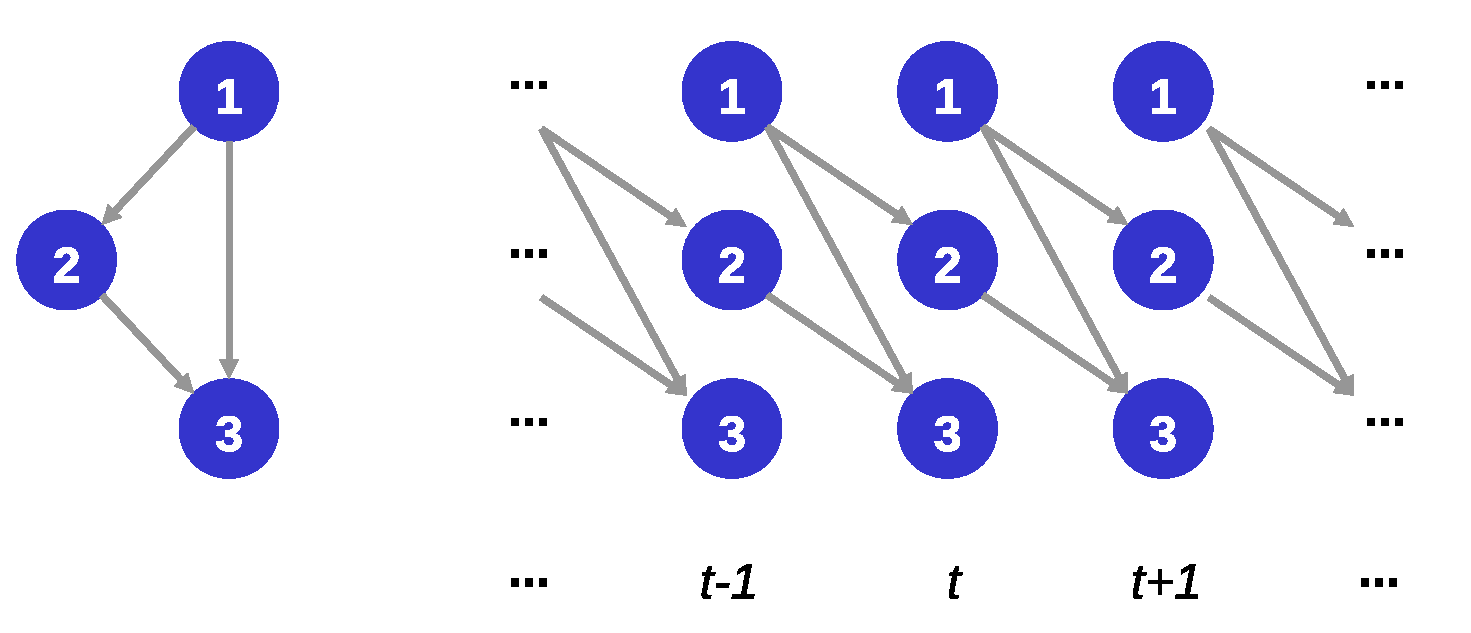
\includegraphics[angle=0, scale=0.50]{feedforwardMotif.eps}
\end{center}
\caption{On the left-hand side: schemata of the feed-forward motif. To the right, the feed-forward motif unfolded. \label{fig.feedforward.motif}}
\end{figure}

\begin{figure}[h!]
\begin{center}
\includegraphics[angle=270, scale=0.50]{feedforward3gene_data.ps}
\end{center}
\caption{Data from  the feed-forward example as specified by model (\ref{form.var1.3gene.feedforward}). The dashed lines connect the data points, the solid line is a smoothing of the data to emphasize the trend. \label{fig.feedforward.data}}
\end{figure}
\clearpage

\end{example}


\subsubsection{Stability and stationarity}
The VAR(1) process is said to be {\it stable} if all eigenvalues of $\mathbf{A}$ have modulus less than one, i.e. $|\lambda_j(\mathbf{A})| < 1$ for $j=1,\ldots,p$. This is equivalent to:
\begin{eqnarray*}
\mbox{det}( \mathbf{I}_{p \times p} - \mathbf{A} \, \mathbf{x}) \not= 0  \qquad \mbox{for } | \mathbf{x} | \leq 1.
\end{eqnarray*}
The process may also be well-defined if the stability does not hold.

The VAR(1) process is said to be {\it strictly stationary} if $P(\mathbf{Y}_{\ast,i,1}, \ldots, \mathbf{Y}_{\ast,i,t} ) = P(\mathbf{Y}_{\ast,i,\tau}, \ldots, \mathbf{Y}_{\ast,i,t+\tau} )$ for any $\tau \in \mathbb{N}$. In words, the joint distribution (i.e. $\mmu_y$ and $\SSigma_y$) does not change over time. In case the definition of strictly stationary is relaxed: the first two moments do not dependent on $t$, the process is referred to as \textit{stationary}.

The two concepts are related by Proposition 2.1 of \cite{Luet2005}: model (\ref{form.var1}) yields a stationary time series if it is stable.
\begin{example}
In Example \ref{example.feedforward.motif} the eigenvalues of $\mathbf{A}$ are $\lambda_j(\mathbf{A}) = 0$ for $j=1, \ldots, p$. Hence, the process is stable, and therefore stationary.
\end{example}


% {\it Question:}
% \\
% Is stationarity something that should be required when modeling cancer development / progression? In the limit, everything goes to pieces: the cancer causes death of the host organism. Carel: may be relevant in case of a chronic disease or no-pregression-plus-no-remission. Mark: can this not be assessed from the data?


\subsubsection{The MA representation}
Assume $\mathbf{Y}_{\ast, i, t}$ follows a VAR(1) model. Then, assuming the model is stable, the process can be represented by:
\begin{eqnarray*}
\mathbf{Y}_{\ast, i, t} & = & \mmu + \sum_{t_0 = 0}^{\infty} \mathbf{A}^{t_0} \vvarepsilon_{t - t_0}
\\
& = & \mmu + \sum_{t_0 = 0}^{\infty} \PPhi_{t_0} \vvarepsilon_{t - t_0}.
\end{eqnarray*}
This is called the {\it moving average (MA) representation} (or sometimes {\it canonical}, {\it fundamental} or {\it prediction error representation}). The representation expresses $\mathbf{Y}_{\ast, i, t}$ in past and present error (innovations). The $\PPhi_{t_0}$ are referred to as the moving average coefficient matrices. The key motivation for this representation is the (more explicit) relation to the mean and autocovariance of the process.




\subsubsection{The structural VAR model}
The \textit{structural VAR(1) model} is a reformulation of the canonical VAR(1) model (\ref{form.var1}) that explicitly takes into account the contemporaneous relationships of the variates that constitute $\mathbf{Y}_{\ast, i, t}$. The structural VAR(1) model that describes the gene expression data from the time-course experiment is:
\begin{eqnarray} \label{form.GMvar1}
\mathbf{Y}_{\ast, i, t} % \, | \, \mathbf{Y}_{\ast, i,t-1}, \ldots,  \mathbf{Y}_{\ast, i, 1}
& = & \mathbf{B} \mathbf{Y}_{\ast, i, t} + \breve{\mathbf{A}} \mathbf{Y}_{\ast, i, t-1} + \breve{\vvarepsilon}_{\ast, i, t},
\end{eqnarray}
where $\breve{\mathbf{A}}$ a $p \times p$ coefficient matrix, $\mathbf{B}$ a $p \times p$ coefficient matrix with a zero diagonal such that $\mathbf{I}_{p \times p} - \mathbf{B}$ is non-singular, and $\breve{\vvarepsilon}_{\ast,i,t}$ a $p \times 1$ vector with the errors. Throughout it is assumed that $\breve{\vvarepsilon}_{\ast,i,t} \sim \mathcal{N}(\mathbf{0}_{p \times 1}, \breve{\mathbf{\Sigma}}_{\varepsilon})$ and $\mbox{Cov}(\breve{\vvarepsilon}_{\ast,i_1,t_1}, \breve{\vvarepsilon}_{\ast,i_2,t_2}) = \mathbf{0}$ if $t_1 \not=t_2$ or $i_1 \not=i_2$. Thus, for a 3-gene pathway model (\ref{form.GMvar1}) becomes:
\begin{eqnarray*}
\left\{
\begin{array}{ccc}
Y_{1,i,t} & = & b_{12} Y_{2,i,t-1} + b_{13} Y_{3,i,t} + \breve{a}_{11} Y_{1,i,t-1} + \breve{a}_{12} Y_{2,i,t-1} + \breve{a}_{13} Y_{3,i,t-1} + \breve{\varepsilon}_{1,i,t},
\\
Y_{2,i,t} & = & b_{21} Y_{1,i,t-1} + b_{23} Y_{3,i,t} + \breve{a}_{21} Y_{1,i,t-1} + \breve{a}_{22} Y_{2,i,t-1} + \breve{a}_{23} Y_{3,i,t-1} + \breve{\varepsilon}_{2,i,t},
\\
Y_{3,i,t} & = & b_{31} Y_{1,i,t-1} + b_{32} Y_{2,i,t} + \breve{a}_{31} Y_{1,i,t-1} + \breve{a}_{32} Y_{2,i,t-1} + \breve{a}_{33} Y_{3,i,t-1} + \breve{\varepsilon}_{3,i,t},
\end{array}
\right.
\end{eqnarray*}
where e.g. $Y_{1,i,t}$ does not appear in the first equations as $b_{11} = 0$.

The relations between the parameters of the canonical and structural VAR(1) models are:
\begin{eqnarray*}
\vvarepsilon_{\ast, i, t} & = & (\mathbf{I}_{p \times p} - \mathbf{B})^{-1} \breve{\vvarepsilon}_{\ast, i, t},
\\
\mathbf{A} & = & (\mathbf{I}_{p \times p} - \mathbf{B})^{-1} \breve{\mathbf{A}},
\\
\SSigma_{\varepsilon}  & = & (\mathbf{I}_{p \times p} - \mathbf{B})^{-1} \breve{\SSigma}_{\varepsilon}
[(\mathbf{I}_{p \times p} - \mathbf{B})^{-1}]^{\mathrm{T}},
\end{eqnarray*}
as the canonical VAR(1) model (\ref{form.var1}) is obtained through pre-multiplication of the structural VAR(1) model (\ref{form.GMvar1})
by $(\mathbf{I}_{p \times p} - \mathbf{B})^{-1}$.


\subsection{Mean, variance, and autocovariance}
Under the above assumptions the vector of gene expression levels of sample $i$ at time point $t$ follows a multivariate normal distribution: $\mathbf{Y}_{\ast, i,t} \sim \mathcal{N}(\mmu_y, \mathbf{\Sigma}_{y})$. The mean of $\mathbf{Y}_{\ast,i,t}$ is:
\begin{eqnarray*}
E(\mathbf{Y}_{\ast,i,t} \, | \, \mathbf{Y}_{\ast,i,t-1}, \ldots,  \mathbf{Y}_{\ast,i,1}) & = & E(\nnu) + \mathbf{A} E\big( \mathbf{Y}_{\ast,i,t-1}\big) + E\big(\vvarepsilon_{\ast,i,t}\big)
\\
& = & \nnu + \mathbf{A}  E\big( \nnu + \mathbf{A} \mathbf{Y}_{\ast,i,t-2}  + \vvarepsilon_{\ast,i,t-1} \big)
\\
& = & \nnu + \mathbf{A} \nnu + \mathbf{A}^2 E\big( \nnu + \mathbf{A} \mathbf{Y}_{\ast,i,t-3}  + \vvarepsilon_{\ast,i,t-2}  \big)
\\
& = & \ldots
\\
& = & \big( \mathbf{I}_{p \times p} + \mathbf{A} + \mathbf{A}^2 + \ldots + \mathbf{A}^{\mathcal{T}-1} \big) \nnu.
\end{eqnarray*}
If $\mathcal{T} \rightarrow \infty$, the mean $\mmu_y$ converges to $\big( \mathbf{I}_{p \times p} - \mathbf{A}\big)^{-1} \nnu$. This assumes that all eigenvalues of $\mathbf{A}$ are smaller than 1 in an absolute sense.

The variance of the process is a little bit more elaborate. Note that from the definition of the model (\ref{form.var1}) it is clear that $\mathbf{\Sigma}_{y}$ satisfies:
\begin{eqnarray} \label{form.lyapunov}
\mathbf{\Sigma}_{y} & = & \mathbf{A} \mathbf{\Sigma}_{y} \mathbf{A}^{\mathrm{T}} + \mathbf{\Sigma}_{\varepsilon}.
\end{eqnarray}
This equation is known as the discrete Lyapunov equation. An analytic solution (solving for $\mathbf{\Sigma}_{y}$) of this equation exists. To arrive at the solution
apply the $\mbox{vec}(\cdot)$ operator, defined by
\begin{eqnarray*}
\mbox{vec}(\mathbf{A})
& = & \mbox{vec} \left( \left(
\begin{array}{cccc}
a_{11} & a_{12} & \ldots & a_{1p}
\\
a_{21} & a_{22} & \ldots & a_{2p}
\\
\vdots & \vdots & \ddots & \vdots
\\
a_{p1} & a_{p2} & \ldots & a_{pp}
\end{array}
\right) \right)
\, \, \, = \, \, \,
(a_{11}, \ldots, a_{p1}, a_{12}, \ldots, a_{p2}, \ldots, a_{1p}, \ldots, a_{pp})^{\mathrm{T}},
\end{eqnarray*}
to both sides of Equation (\ref{form.lyapunov}):
\begin{eqnarray*}
\mbox{vec}(\mathbf{\Sigma}_{\varepsilon}) & = &
\mbox{vec}(\mathbf{\Sigma}_{y}) - \mbox{vec}(\mathbf{A} \mathbf{\Sigma}_{y} \mathbf{A}^{\mathrm{T}})
\\
& = &
\mbox{vec}(\mathbf{\Sigma}_{y}) - (\mathbf{A} \otimes \mathbf{A} )
\mbox{vec}(\mathbf{\Sigma}_{y})
\\
& = & (\mathbf{I}_{p^2 \times p^2} - \mathbf{A} \otimes \mathbf{A} )
\mbox{vec}(\mathbf{\Sigma}_{y}),
\end{eqnarray*}
where the identity $\mbox{vec}( \mathbf{A} \mathbf{B} \mathbf{C}) = (\mathbf{C}^{\mathrm{T}} \otimes \mathbf{A}) \mbox{vec}( \mathbf{B})$ is used. Thus:
\begin{eqnarray*}
\mbox{vec}(\mathbf{\Sigma}_{y}) & = & (\mathbf{I}_{p^2 \times p^2} - \mathbf{A} \otimes \mathbf{A} )^{-1} \, \mbox{vec}(\mathbf{\Sigma}_{\varepsilon}),
\end{eqnarray*}
presuming the inverse exists. With respect to this existence note that {\it i)} the eigenvalues of $\mathbf{A} \otimes \mathbf{A}$ are given by $\lambda_{j_1}(\mathbf{A}) \lambda_{j_2}(\mathbf{A})$ for $j_1, j_2=1,\ldots,p$, and {\it ii)} the eigenvalues of $\mathbf{I}_{p^2 \times p^2} - \mathbf{A} \otimes \mathbf{A}$ are then of the form $1 - \lambda_{j_1}(\mathbf{A}) \lambda_{j_2}(\mathbf{A})$. Consequently, the inverse (and thus the solution) above exists if for any eigenvalue of $\mathbf{A}$ its reciprocal is not an eigenvalue of $\mathbf{A}$.
% and $\lambda_{j_1}(\mathbf{A}) \lambda_{j_2}(\mathbf{A}) \not= 1$ for any combination of $j_1$ and $j_2$.
\\
\\
A well-known alternative solution of the discrete Lyapunov equation (\ref{form.lyapunov}) is:
\begin{eqnarray*}
\mathbf{\Sigma}_{y} & = & \sum_{k=0}^{\infty} \mathbf{A}^k \mathbf{\Sigma}_{\varepsilon} (\mathbf{A}^{\mathrm{T}})^k.
\end{eqnarray*}
To see this is indeed a solution of the discrete Lyapunov equation, simply substitute it:
\begin{eqnarray*}
\sum_{k=0}^{\infty} \mathbf{A}^k \mathbf{\Sigma}_{\varepsilon} (\mathbf{A}^{\mathrm{T}})^k & = & \mathbf{A} \Big( \sum_{k=0}^{\infty} \mathbf{A}^k \mathbf{\Sigma}_{\varepsilon} (\mathbf{A}^{\mathrm{T}})^k \Big) \mathbf{A}^{\mathrm{T}} + \mathbf{\Sigma}_{\varepsilon}
\\
& = & \sum_{k=1}^{\infty} \mathbf{A}^k \mathbf{\Sigma}_{\varepsilon} (\mathbf{A}^{\mathrm{T}})^k + \mathbf{\Sigma}_{\varepsilon} \, \, \, =
\, \, \, \sum_{k=0}^{\infty} \mathbf{A}^k \mathbf{\Sigma}_{\varepsilon} (\mathbf{A}^{\mathrm{T}})^k.
\end{eqnarray*}
Furthermore, the positive-definiteness of $\mathbf{\Sigma}_{\varepsilon}$ warrants the positive-definiteness of $\mathbf{\Sigma}_{y}$ (this follows directly from iterative application of results from \citealt{Har2008}). \reminder{Quote proposition number from Harville.}

We now investigate the convergence of this series solution. Hereto diagonalize $\mathbf{A}$ by means of its eigen-decomposition $\mathbf{A} = \mathbf{V}_a \mathbf{D}_a \mathbf{V}^{-1}_a$. The discrete Lyapunov equation then becomes:
\begin{eqnarray*}
\mathbf{\Sigma}_{y} & = & \mathbf{V}_a \mathbf{D}_a \mathbf{V}^{-1}_a \mathbf{\Sigma}_{y} ( \mathbf{V}_a^{-1})^{\mathrm{T}} \mathbf{D}_a \mathbf{V}^{\mathrm{T}}_a  + \mathbf{\Sigma}_{\varepsilon}.
\end{eqnarray*}
Or, reformulated:
\begin{eqnarray*}
\tilde{\mathbf{\Sigma}}_{y} & = & \mathbf{D}_a  \tilde{\mathbf{\Sigma}}_{y} \mathbf{D}_a  + \tilde{\mathbf{\Sigma}}_{\varepsilon},
\end{eqnarray*}
where $\tilde{\mathbf{\Sigma}}_{y}  = \mathbf{V}_a^{-1}  \mathbf{\Sigma}_{y} (\mathbf{V}_a^{-1})^{\mathrm{T}}$ and $\tilde{\mathbf{\Sigma}}_{\varepsilon} = \mathbf{V}_a^{-1}  \mathbf{\Sigma}_{\varepsilon} (\mathbf{V}_a^{-1})^{\mathrm{T}}$. The solution of this reformulated discrete Lyapunov equation is:
\begin{eqnarray*}
\tilde{\mathbf{\Sigma}}_{y} & = & \sum_{k=0}^{\infty} \mathbf{D}_a^k \tilde{\mathbf{\Sigma}}_{\varepsilon} \mathbf{D}_a^k.
\end{eqnarray*}
Or, in terms of the elements of the matrices:
\begin{eqnarray*}
(\tilde{\mathbf{\Sigma}}_{y})_{j_1, j_2} & = & \sum_{k=0}^{\infty} (\mathbf{D}_a^k \tilde{\mathbf{\Sigma}}_{\varepsilon} \mathbf{D}_a^k)_{j_1, j_2}
\\
&  = & (\tilde{\mathbf{\Sigma}}_{\varepsilon})_{j_1, j_2} \sum_{k=0}^{\infty} [(\mathbf{D}_a)_{j_1, j_1}  (\mathbf{D}_a)_{j_2, j_2}]^k
\\
&  = &  \frac{(\tilde{\mathbf{\Sigma}}_{\varepsilon})_{j_1, j_2}}{ 1 - (\mathbf{D}_a)_{j_1, j_1}  (\mathbf{D}_a)_{j_2, j_2}},
\end{eqnarray*}
where we have used that $\mathbf{D}$ is diagonal. If one defines a $p \times p$ matrix $\mathbf{C}$ with $(\mathbf{C})_{j_1, j_2} = [1 - (\mathbf{D}_a)_{j_1, j_1}  (\mathbf{D}_a)_{j_2, j_2}]^{-1}$, then:
\begin{eqnarray*}
\mathbf{\Sigma}_y & = & \mathbf{V}_a (\tilde{\mathbf{\Sigma}}_{\varepsilon} \circ \mathbf{C}) \mathbf{V}_a^{\mathrm{T}},
\end{eqnarray*}
where the $\circ$ operator indicates the Hadamard product. From the above it should also be clear that $\mathbf{\Sigma}_y$ is well-defined by the series solution if $\lambda_{j_1}(\mathbf{A}) \not= [\lambda_{j_2}(\mathbf{A})]^{-1}$ for any couple $j_1$ and $j_2$.

\begin{example} \textit{Mean and variance of the feedforward motif.}
Revisit Example \ref{example.feedforward.motif}. Clearly, as $\nnu = \mathbf{0}_{p \times 1}$, the mean $\mmu$ also equals $\mathbf{0}_{p \times 1}$. The variance of $\mathbf{Y}_{\ast, i, t}$ is:
\begin{eqnarray*}
\SSigma_{y} & = &
\left(
\begin{array}{rrr}
0.2500 & 0.0000 & 0.0000
\\
0.0000 & 1.8125 & -1.1250
\\
0.0000 & -1.1250 & 5.1381
\end{array}
\right),
\end{eqnarray*}
where numbers have been rounded.
\end{example}
\mbox{ }
\\
\\
Now we have defined the mean and variance of the time series process, the remaining interesting quantity in VAR(1) model is the autocovariance. The {\it autocovariance} is the covariance between the gene expression profile at time point $t$ and that at some other time point. The autocovariance of the VAR(1) process is (for $\tau \geq 0$):
\begin{eqnarray*}
\mathbf{\Gamma}(\tau) & = & \mbox{Cov} \big( \mathbf{Y}_{\ast,i,t}, \mathbf{Y}_{\ast,i,t+\tau} \big)
\, \, \, = \, \, \, E\Big[ \big(\mathbf{Y}_{\ast,i,t} - E(\mathbf{Y}_{\ast,i,t}) \big) \big(\mathbf{Y}_{\ast,i,t+\tau} - E(\mathbf{Y}_{\ast,i,t+\tau}) \big)^{\mathrm{T}} \Big]
% \\
% & = & E\Big[ \Big(\mathbf{Y}_{\ast i}^{(t)} - E(\mathbf{Y}_{\ast i}^{(t)}) \big)
% \\
% & &
% \Big( \sum_{k=0}^{\tau-1} \mathbf{A}^k \nnu + \mathbf{A}^{\tau} \mathbf{Y}_{\ast i}^{(t)} + \sum_{k=0}^{\tau-1} \mathbf{A}^k \vvarepsilon_{\ast i}^{(t+\tau-k)}- E \Big(\sum_{k=0}^{\tau-1} \mathbf{A}^k \nnu + \mathbf{A}^{\tau} \mathbf{Y}_{\ast i}^{(t)} + \sum_{k=0}^{\tau-1} \mathbf{A}^k \vvarepsilon_{\ast i}^{(t+\tau-k)} \Big) \Big)^T \Big]
\\
& = & E\Big[ \Big(\mathbf{Y}_{\ast,i,t)} - E(\mathbf{Y}_{\ast,i,t}) \big) \Big( \mathbf{A}^{\tau} \mathbf{Y}_{\ast,i,t} + \sum_{k=0}^{\tau-1} \mathbf{A}^k \vvarepsilon_{\ast,i,t+\tau-k} - E \big(\mathbf{A}^{\tau} \mathbf{Y}_{\ast,i,t} \big) \Big)^{\mathrm{T}} \Big]
\\
& = & E \Big[ \big(\mathbf{Y}_{\ast,i,t} - E(\mathbf{Y}_{\ast,i,t}) \big) \big( \mathbf{A}^{\tau} \mathbf{Y}_{\ast,i,t} - E(\mathbf{A}^{\tau} \mathbf{Y}_{\ast,i,t}) \big)^{\mathrm{T}} \Big]
\, \, \, = \, \, \, \mbox{Cov} \big( \mathbf{Y}_{\ast,i,t}, \mathbf{Y}_{\ast,i,t} \big) [\mathbf{A}^{\tau}]^{\mathrm{T}}
\\
& = & \SSigma_y [\mathbf{A}^{\tau}]^{\mathrm{T}}.
\end{eqnarray*}
Similarly, for $\tau < 0$:
\begin{eqnarray*}
\mathbf{\Gamma}(\tau) \, \, \, = \, \, \,  \mbox{Cov} \big( \mathbf{Y}_{\ast,i,t-\tau}, \mathbf{Y}_{\ast,i,t} \big) & = & \mathbf{A}^{-\tau} \SSigma_y.
\end{eqnarray*}
In the above it is used that $\mbox{Cov} \big( \vvarepsilon_{\ast,i,t}, \vvarepsilon_{\ast,i,t+\tau} \big) = 0$ if $\tau \not= 0$.

Associated with the autocovariance matrix are the {\it autocorrelation} and {\it crosscorrelation} (or sometimes {\it cross-autocorrelation}). Crosscorrelation is defined as $\mbox{Cor}(Y_{j_1,i,t}, Y_{j_2,i,t+\tau})$ for $j_1 \not= j_2$ and $\tau \in \mathbb{N}$. The crosscorrelation is thus the correlation with lag $\tau$ between the time series of two different genes. The autocorrelation is reserved for the special case where $j_1 = j_2$. In the autocovariance matrix for the VAR(1) process, the diagonal elements are thus proportional to the autocorrelations and the off-diagonal elements to the crosscorrelations.

Finally, another frequently used quantity in times series is the {\it partial autocorrelation}. This is defined as:
\begin{eqnarray*}
\mbox{Cor}(Y_{j,i,t}, Y_{j,i,t+\tau} \, | \, Y_{j,i,t+1}, \ldots, Y_{j,i,t+\tau-1}).
\end{eqnarray*}
Hence, the correlation between the expression levels of a gene at two time points which is not propagated via the intermediate time points. The partial autocorrelation is used to determine the lag of the time series. As we assume the lag to equal one throughout, the partial autocovariance and partial autocorrelation appear to be of little interest here.



\subsection{Estimation}
\subsubsection{Mean and autocovariance}
The process mean is estimated by:
\begin{eqnarray*}
\hat{\mmu}_y & = & \frac{1}{n\mathcal{T}} \sum_{i=1}^n \sum_{t=1}^{\mathcal{T}} \mathbf{Y}_{\ast,i,t},
\end{eqnarray*}
which has the following expectation:
\begin{eqnarray*}
E(\hat{\mmu}_y) & = & \frac{1}{n\mathcal{T}} \sum_{i=1}^n \sum_{t=1}^{\mathcal{T}} E( \mathbf{Y}_{\ast,i,t} ) \, \, \, = \, \, \, \frac{1}{n\mathcal{T}} \sum_{i=1}^n \sum_{t=1}^{\mathcal{T}} \mmu_y
\, \, \, = \, \, \,  \mmu_y.
\end{eqnarray*}
Hence, the estimator for the mean is unbiased.

A natural estimator for the autocovariance (confer \citealt{Broc2006}) would be:
\begin{eqnarray*}
\hat{\mathbf{\Gamma}}(\tau) & = &
\left\{
\begin{array}{rcccl}
\frac{1}{n(\mathcal{T}-\tau)} \sum_{i=1}^n \sum_{t=1}^{\mathcal{T}-\tau} ( \mathbf{Y}_{\ast,i,t} - \hat{\mmu}_y) \big(\mathbf{Y}_{\ast,i,t+\tau} - \hat{\mmu}_y \big)^{\mathrm{T}} & & \mbox{for} & 0 \leq \tau  \leq \mathcal{T}-1,
\\
\frac{1}{n(\mathcal{T}-\tau)} \sum_{i=1}^n \sum_{t=-\tau+1}^{\mathcal{T}} ( \mathbf{Y}_{\ast,i,t} - \hat{\mmu}_y) \big(\mathbf{Y}_{\ast,i,t+\tau} - \hat{\mmu}_y \big)^{\mathrm{T}} & & \mbox{for} & -\mathcal{T}+1 \leq \tau  < 0.
\end{array}
\right.
\end{eqnarray*}
However, as we have centered the data, we consider the following estimator:
\begin{eqnarray*}
\hat{\mathbf{\Gamma}}(\tau) & = &
\left\{
\begin{array}{rcccl}
\frac{1}{n(\mathcal{T}-\tau)} \sum_{i=1}^n \sum_{t=1}^{\mathcal{T}-\tau}  \mathbf{Y}_{\ast,i,t} \mathbf{Y}_{\ast,i,t+\tau}^{\mathrm{T}} & & \mbox{for} & 0 \leq \tau  \leq \mathcal{T}-1,
\\
\frac{1}{n(\mathcal{T}-\tau)} \sum_{i=1}^n \sum_{t=-\tau+1}^{\mathcal{T}} \mathbf{Y}_{\ast,i,t} \mathbf{Y}_{\ast,i,t+\tau}^{\mathrm{T}} & &
\mbox{for} & -\mathcal{T}+1 \leq \tau  < 0.
\end{array}
\right.
\end{eqnarray*}
For the calculation of the expectation of the covariance estimator we thus assume that $\mmu_y=0$ (as we have centered the gene expression levels around zero).
Then, for $\tau \geq 0$, we have:
\begin{eqnarray*}
E[ \hat{\mathbf{\Gamma}}(\tau) ] & = & \frac{1}{n(\mathcal{T}-\tau)} \sum_{i=1}^n \sum_{t=1}^{\mathcal{T}-\tau} E[ \mathbf{Y}_{\ast,i,t} \mathbf{Y}_{\ast,i,t+\tau}^{\mathrm{T}} ]
\, \, \, = \, \, \, \GGamma(\tau) .
\end{eqnarray*}
Again, an unbiased estimator. Note that expectation of the `natural' autocovariance estimator of \cite{Broc2006} is not unbiased. It is however consistent.
\\
\\
\reminder{Mark: When $\mu_y$  is assumed  to be zero, the degrees of freedom also changes. Hence, divide by $n \mathcal{T}$ rather than $n(\mathcal{T}-\tau)$! }

% {\it Question:} Is it reasonable to assume the alternative autocovariance estimator?




\subsubsection{Model parameters $\mathbf{A}$ and $\SSigma_{\varepsilon}$}
We now turn to the estimation of the parameters of model (\ref{form.var1}). This is done by likelihood maximization. It should be noted that the ML estimators for $\mathbf{A}$ coincides with that of the least squares approach. As we have centered (per gene, within each sample) the expression values, we may consider $\nnu = \mathbf{0}$. Thus, $\mathbf{Y}_{\ast,i,t} \, | \, \mathbf{Y}_{\ast,i,t-1}, \ldots,  \mathbf{Y}_{\ast,i,1}  \sim \mathcal{N}( \mathbf{A} \mathbf{Y}_{\ast,i,t}  , \SSigma_{\varepsilon})$. The likelihood is then:
\begin{eqnarray*}
& & \hspace{-1cm} L(\mathbf{Y}; \nnu, \mathbf{A}, \SSigma_{\varepsilon})
\\
& = & \prod_{i=1}^n P(\mathbf{Y}_{\ast,i,\mathcal{T}}, \ldots, \mathbf{Y}_{\ast,i,1})
\, \, \,  = \, \, \, \prod_{i=1}^n
\prod_{t=1}^{\mathcal{T}} P(\mathbf{Y}_{\ast,i,t} \, | \, \mathbf{Y}_{\ast,i,t-1}, \ldots, \mathbf{Y}_{\ast,i,1})
\\
& = & \prod_{i=1}^n \prod_{t=2}^{\mathcal{T}} \frac{1}{(2\pi)^{p/2} | \SSigma_{\varepsilon} |^{1/2} } \exp \big[ - \big( \mathbf{Y}_{\ast,i,t} - \mathbf{A} \mathbf{Y}_{\ast,i,t-1}  \big)^\mathrm{T} \SSigma_{\varepsilon}^{-1} \big(\mathbf{Y}_{\ast,i,t} - \mathbf{A} \mathbf{Y}_{\ast,i,t-1}  \big) \big]
\\
& = & \prod_{i=1}^n \prod_{t=2}^{\mathcal{T}} \frac{1}{(2\pi)^{p/2} | \SSigma_{\varepsilon} |^{1/2} }  \exp \big\{ - \big[ \mathbf{Y}_{\ast,i,t} -
\big( \mathbf{Y}_{\ast,i,t-1}^{\mathrm{T}}  \otimes \mathbf{I}_{p \times p} \big) \mbox{vec}(\mathbf{A})  \big]^{\mathrm{T}}
\\
& & \qquad \qquad \qquad \qquad  \qquad \qquad \qquad \, \SSigma_{\varepsilon}^{-1} \big[ \mathbf{Y}_{\ast,i,t} -
\big( \mathbf{Y}_{\ast,i,t-1}^\mathrm{T}  \otimes \mathbf{I}_{p \times p} \big) \mbox{vec}(\mathbf{A})  \big] \big\}
\end{eqnarray*}
% For the estimation of $\mathbf{A}$, we select only the part of the log-likelihood that involves $\mbox{vec}(\mathbf{A})$:
% \begin{eqnarray*}
% - \frac{1}{2}  \sum_{i=1}^n \sum_{t=1}^T  \big[ \mathbf{Y}_{\ast i}^{(t)} - \nnu -
% \big( \big( \mathbf{Y}_{\ast i}^{(t-1)} \big)^T  \otimes \mathbf{I}_{p \times p} \big) \mbox{vec}(\mathbf{A})  \big]^T
% \SSigma_{\varepsilon}^{-1} \big[ \mathbf{Y}_{\ast i}^{(t)} - \nnu -
% \big( \big( \mathbf{Y}_{\ast i}^{(t-1)} \big)^T  \otimes \mathbf{I}_{p \times p} \big) \mbox{vec}(\mathbf{A})  \big]
% \end{eqnarray*}
Equate the derivative of the log-likelihood with respect to $\mbox{vec}(\mathbf{A})$ to zero:
\begin{eqnarray*}
0 & = & \sum_{i=1}^n \sum_{t=2}^{\mathcal{T}} \big( \mathbf{Y}_{\ast,i,t-1}^{\mathrm{T}}  \otimes \mathbf{I}_{p \times p} \big)^{\mathrm{T}}  \SSigma_{\varepsilon}^{-1}
\big(\mathbf{Y}_{\ast,i,t} - \big( \mathbf{Y}_{\ast,i,t-1}^{\mathrm{T}}  \otimes \mathbf{I}_{p \times p} \big) \mbox{vec}(\mathbf{A}) \big).
% \\
% & = & \sum_{i=1}^n \sum_{t=1}^T \big( \mathbf{Y}_{\ast i}^{(t-1)}   \otimes \mathbf{I}_{p \times p} \big)  \SSigma_{\varepsilon}^{-1}
% \big(\mathbf{Y}_{\ast i}^{(t)} - \nnu - \big( \big( \mathbf{Y}_{\ast i}^{(t-1)} \big)^T  \otimes \mathbf{I}_{p \times p} \big) \mbox{vec}(\mathbf{A}) \big)
% \\
% & = & \sum_{i=1}^n \sum_{t=1}^T \big( \mathbf{Y}_{\ast i}^{(t-1)}   \otimes \mathbf{I}_{p \times p} \big) \big( 1 \otimes \SSigma_{\varepsilon}^{-1})
% \big(\mathbf{Y}_{\ast i}^{(t)} - \nnu - \big( \big( \mathbf{Y}_{\ast i}^{(t-1)} \big)^T  \otimes \mathbf{I}_{p \times p} \big) \mbox{vec}(\mathbf{A}) \big)
% \\
% & = & \sum_{i=1}^n \sum_{t=1}^T \big( \mathbf{Y}_{\ast i}^{(t-1)}  \otimes \SSigma_{\varepsilon}^{-1})
% \big(\mathbf{Y}_{\ast i}^{(t)} - \nnu - \big( \big( \mathbf{Y}_{\ast i}^{(t-1)} \big)^T  \otimes \mathbf{I}_{p \times p} \big) \mbox{vec}(\mathbf{A}) \big)
% \\
% & = & \sum_{i=1}^n \sum_{t=1}^T \big( \mathbf{Y}_{\ast i}^{(t-1)}  \otimes \SSigma_{\varepsilon}^{-1}\big)
% \big(\mathbf{Y}_{\ast i}^{(t)} - \nnu \big) -
% \sum_{i=1}^n \sum_{t=1}^T \big( \mathbf{Y}_{\ast i}^{(t-1)}  \otimes \SSigma_{\varepsilon}^{-1}\big) \big( \big( \mathbf{Y}_{\ast i}^{(t-1)} \big)^T  \otimes \mathbf{I}_{p \times p} \big) % \mbox{vec}(\mathbf{A})
% \\
% & = & \sum_{i=1}^n \sum_{t=1}^T \big( \mathbf{Y}_{\ast i}^{(t-1)}  \otimes \SSigma_{\varepsilon}^{-1}\big)
% \big(\mathbf{Y}_{\ast i}^{(t)} - \nnu \big) -
% \sum_{i=1}^n \sum_{t=1}^T \big( \mathbf{Y}_{\ast i}^{(t-1)} \big( \mathbf{Y}_{\ast i}^{(t-1)} \big)^T \otimes \SSigma_{\varepsilon}^{-1}\big) \mbox{vec}(\mathbf{A})
% \\
% & = & \big( 1 \otimes \SSigma_{\varepsilon}^{-1}\big) \sum_{i=1}^n \sum_{t=1}^T \big( \mathbf{Y}_{\ast i}^{(t-1)}  \otimes \mathbf{I}_{p \times p} \big)
% \big(\mathbf{Y}_{\ast i}^{(t)} - \nnu \big)
% \\
% & & \quad - \, \, \big( 1 \otimes \SSigma_{\varepsilon}^{-1}\big)  \sum_{i=1}^n \sum_{t=1}^T \big( \mathbf{Y}_{\ast i}^{(t-1)} \big( \mathbf{Y}_{\ast i}^{(t-1)} \big)^T \otimes \mathbf{I}_{p \times p} \big) \mbox{vec}(\mathbf{A})
% \\
% \big( 1 \otimes \SSigma_{\varepsilon}^{-1}\big) \sum_{i=1}^n \sum_{t=1}^T \big( \mathbf{Y}_{\ast i}^{(t-1)}  \otimes \mathbf{I}_{p \times p} \big)
% \big(\mathbf{Y}_{\ast i}^{(t)} - \nnu \big)
% & = & \big( 1 \otimes \SSigma_{\varepsilon}^{-1}\big)  \big( \sum_{i=1}^n \sum_{t=1}^T \mathbf{Y}_{\ast i}^{(t-1)} \big( \mathbf{Y}_{\ast i}^{(t-1)} \big)^T \otimes \mathbf{I}_{p \times p} \big) \mbox{vec}(\mathbf{A}).
\end{eqnarray*}
After some algebraic manipulations this is rewritten to:
\begin{eqnarray*}
0 & = & \sum_{i=1}^n \sum_{t=2}^{\mathcal{T}} \big( \mathbf{Y}_{\ast,i,t-1}  \otimes \SSigma_{\varepsilon}^{-1}\big)
\mathbf{Y}_{\ast,i,t} -
\sum_{i=1}^n \sum_{t=1}^{\mathcal{T}} \big( \mathbf{Y}_{\ast,i,t-1} \mathbf{Y}_{\ast,i,t-1}^{\mathrm{T}} \otimes \SSigma_{\varepsilon}^{-1}\big) \mbox{vec}(\mathbf{A}).
\end{eqnarray*}
Solve this estimation equation to obtain an estimate for $\mathbf{A}$:
\begin{eqnarray*}
\mbox{vec}(\hat{\mathbf{A}}) & = &
\Big(
\sum_{i=1}^n \sum_{t=2}^{\mathcal{T}} \mathbf{Y}_{\ast,i,t-1} \mathbf{Y}_{\ast,i,t-1}^{\mathrm{T}} \otimes \mathbf{I}_{p \times p}
\Big)^{-1}
\sum_{i=1}^n \sum_{t=2}^{\mathcal{T}} \big( \mathbf{Y}_{\ast,i,t-1}  \otimes \mathbf{I}_{p \times p} \big)
\big(\mathbf{Y}_{\ast,i,t}\big).
\end{eqnarray*}
Notice that this expression can be formulated differently:
\begin{eqnarray*}
\hat{\mathbf{A}} & = &  \Big[ \frac{1}{n(\mathcal{T}-1)} \sum_{i=1}^n \sum_{t=1}^{\mathcal{T}-1}  \mathbf{Y}_{\ast,i,t+1} \mathbf{Y}_{\ast,i,t}^{\mathrm{T}} \Big] \Big[ \frac{1}{n({\mathcal{T}}-1)} \sum_{i=1}^n \sum_{t=1}^{{\mathcal{T}}-1}  \mathbf{Y}_{\ast,i,t} \mathbf{Y}_{\ast,i,t}^{\mathrm{T}} \Big]^{-1}
\end{eqnarray*}
This is a more convenient expression when dealing with high-dimensional data.

Finally, the estimator for $\SSigma_{\varepsilon}$ is given by:
\begin{eqnarray*}
\hat{\SSigma}_{\varepsilon} & = & \frac{1}{n \mathcal{T}}  \sum_{i=1}^n \sum_{t=2}^{\mathcal{T}}  \big[ \mathbf{Y}_{\ast,i,t} - \big( \mathbf{Y}_{\ast, i,t-1}^{\mathrm{T}}  \otimes \mathbf{I}_{p \times p} \big) \mbox{vec}(\mathbf{A})  \big] \big[ \mathbf{Y}_{\ast,i,t} - \big( \mathbf{Y}_{\ast,i,t-1}^{\mathrm{T}}  \otimes \mathbf{I}_{p \times p} \big) \mbox{vec}(\mathbf{A})  \big]^{\mathrm{T}}
\\
& = & \frac{1}{n \mathcal{T}}  \sum_{i=1}^n \sum_{t=2}^{\mathcal{T}}  \big[ \mathbf{Y}_{\ast,i,t} - \mathbf{A} \mathbf{Y}_{\ast,i,t-1}  \big] \big[ \mathbf{Y}_{\ast,i,t} - \mathbf{A} \mathbf{Y}_{\ast,i,t-1}  \big]^{\mathrm{T}}.
\end{eqnarray*}
Thus, $\SSigma_{\varepsilon}$ is simply estimated by the sample residual covariance matrix.



\subsubsection{Bias of the OLS/ML estimator of $\mathbf{A}$}
For small $\mathcal{T}$, exactly the case we usually encounter, the OLS and ML estimator of $\mathbf{A}$, as derived above, are biased. An explicit expression of the bias of the `natural estimator' of $\mathbf{A}$ in the VAR(1) model with $n=1$ has been derived by \cite{Nich1988}. A sketch of their  approach follows. Define:
\begin{eqnarray*}
\hat{\mathbf{\Gamma}}_{\mathcal{T}} (\tau) & = &  \frac{1}{n(\mathcal{T}-\tau)} \sum_{i=1}^n \sum_{t=1}^{\mathcal{T}-\tau}  \mathbf{Y}_{\ast,i,t} \mathbf{Y}_{\ast,i,t+\tau}^{\mathrm{T}},
\end{eqnarray*}
where $\tau = -1$ or $\tau = 0$. Furthermore, define the random variables:
\begin{eqnarray*}
\mathbf{P}_{\mathcal{T}} & = & \big[ \hat{\mathbf{\Gamma}}_{\mathcal{T}}(-1) - \mathbf{\Gamma}(-1) \big] [\mathbf{\Gamma}(0)]^{-1}
\\
\mathbf{Q}_{\mathcal{T}} & = & \big[ \hat{\mathbf{\Gamma}}_{\mathcal{T}}(0) - \mathbf{\Gamma}(0) \big] [\mathbf{\Gamma}(0)]^{-1} \, \, \, = \, \, \,
\hat{\mathbf{\Gamma}}_{\mathcal{T}}(0) [\mathbf{\Gamma}(0)]^{-1} - \mathbf{I}_{p \times p}.
\end{eqnarray*}
The estimator of $\mathbf{A}$ can then be written as:
\begin{eqnarray*}
\hat{\mathbf{A}}_{\mathcal{T}} & = &  \hat{\mathbf{\Gamma}}_{\mathcal{T}}(-1) \big[ \hat{\mathbf{\Gamma}}_{\mathcal{T}}(0) ]^{-1}
\\
& = & \hat{\mathbf{\Gamma}}_{\mathcal{T}}(-1) \big[ \hat{\mathbf{\Gamma}}_{\mathcal{T}}(0) ]^{-1}  +  \mathbf{A} \mathbf{\Gamma}(0) [\hat{\mathbf{\Gamma}}_{\mathcal{T}}(0)]^{-1}   - \mathbf{\Gamma}(-1) [\hat{\mathbf{\Gamma}}_{\mathcal{T}}(0)]^{-1}
\\
& = & \hat{\mathbf{\Gamma}}_{\mathcal{T}}(-1) [\mathbf{\Gamma}(0)]^{-1}  \mathbf{\Gamma}(0) \big[ \hat{\mathbf{\Gamma}}_{\mathcal{T}}(0) ]^{-1} +  \mathbf{A} (\mathbf{I}_{p \times p} + \mathbf{Q}_{\mathcal{T}})^{-1}  - \mathbf{\Gamma}(-1) [\mathbf{\Gamma}(0)]^{-1} \mathbf{\Gamma}(0)  [\hat{\mathbf{\Gamma}}_{\mathcal{T}}(0)]^{-1}
\\
& = & \{ \hat{\mathbf{\Gamma}}_{\mathcal{T}}(-1) [\mathbf{\Gamma}(0)]^{-1}   - \mathbf{\Gamma}(-1) [\mathbf{\Gamma}(0)]^{-1}  \}
\mathbf{\Gamma}(0)  \big[ \hat{\mathbf{\Gamma}}_{\mathcal{T}}(0) \big]^{-1} +  \mathbf{A} (\mathbf{I}_{p \times p} + \mathbf{Q}_{\mathcal{T}})^{-1}
\\
& = & (\mathbf{A} + \mathbf{P}_{\mathcal{T}}) (\mathbf{I}_{p \times p} + \mathbf{Q}_{\mathcal{T}})^{-1}
\\
& = & (\mathbf{A} + \mathbf{P}_{\mathcal{T}} )  \sum_{k=0}^{\infty} (-1)^k \mathbf{Q}_{\mathcal{T}}^k
\\
& = &  \mathbf{A} + \mathbf{P}_{\mathcal{T}} - \mathbf{A} \mathbf{Q}_{\mathcal{T}}   - \mathbf{P}_{\mathcal{T}} \mathbf{Q}_{\mathcal{T}}  + \mathbf{A} \mathbf{Q}_{\mathcal{T}}^2   + \mathbf{P}_{\mathcal{T}} \mathbf{Q}_{\mathcal{T}}^2  + \ldots
\end{eqnarray*}
Now take the expectation on both sides:
\begin{eqnarray*}
E( \hat{\mathbf{A}}_{\mathcal{T}} ) & = &  \mathbf{A} + E(\mathbf{P}_{\mathcal{T}}) - E(\mathbf{A} \mathbf{Q}_{\mathcal{T}} )  - E(\mathbf{P}_{\mathcal{T}} \mathbf{Q}_{\mathcal{T}})  + E(\mathbf{A} \mathbf{Q}_{\mathcal{T}}^2)   + E(\mathbf{P}_{\mathcal{T}} \mathbf{Q}_{\mathcal{T}}^2)  + \ldots
\\
& = &  \mathbf{A} + E(\mathbf{P}_{\mathcal{T}} \mathbf{Q}_{\mathcal{T}})  + E(\mathbf{A} \mathbf{Q}_{\mathcal{T}}^2)   + E(\mathbf{P}_{\mathcal{T}} \mathbf{Q}_{\mathcal{T}}^2)  + \ldots
\end{eqnarray*}
The remaining expectation are not (necessarily) zero, hence the OLS / ML estimator of $\mathbf{A}$ is biased \citep{Nich1988}. However, it is consistent \citep{Luet2005}.

\subsubsection{Estimation with constraints on $\mathbf{A}$}
Add constraints. In particular, the sign of the coefficients may be known. Hence, work out details.


\subsubsection{Ridge estimation}
The ridge estimator for $\mathbf{A}$ is readily obtained by subtracting the term $\frac{1}{2} \mbox{tr}[\mbox{vec}(\mathbf{A})^\mathrm{T} \LLambda \mbox{vec}(\mathbf{A})]$ from the log-likelihood. In case $\LLambda = \lambda \mathbf{I}_{p^2 \times p^2}$ the penalty reduces to $\frac{\lambda}{2} \mbox{tr}[\mbox{vec}(\mathbf{A})^\mathrm{T} \LLambda \mbox{vec}(\mathbf{A})] = \frac{\lambda}{2} \| \mathbf{A} \|_2^2 = \frac{\lambda}{2} \sum_{j_1, j_2 = 1}^p (\mathbf{A})_{j_1, j_2}^2$.
The ridge estimator thus becomes:
\begin{eqnarray*}
\mbox{vec}[\hat{\mathbf{A}}(\lambda)] & = &
\Big(\lambda \mathbf{I}_{p^2 \times p^2} +
\sum_{i=1}^n \sum_{t=2}^{\mathcal{T}} \mathbf{Y}_{\ast,i,t-1} \mathbf{Y}_{\ast,i,t-1}^{\mathrm{T}} \otimes \mathbf{I}_{p \times p}
\Big)^{-1}
\sum_{i=1}^n \sum_{t=2}^{\mathcal{T}} \big( \mathbf{Y}_{\ast,i,t-1}  \otimes \mathbf{I}_{p \times p} \big)
\big(\mathbf{Y}_{\ast,i,t} - \nnu \big).
\end{eqnarray*}
Or, when we use the more efficient formulation of the estimator if $\mathbf{A}$ and write $\LLambda = \lambda \mathbf{I}_{p \times p}$:
\begin{eqnarray} \label{form.ridge.estimator}
\hat{\mathbf{A}}(\lambda) & = &  \Big( \frac{1}{n(\mathcal{T}-1)} \sum_{i=1}^n \sum_{t=1}^{\mathcal{T}-1}  \mathbf{Y}_{\ast,i,t+1} \mathbf{Y}_{\ast,i,t}^{\mathrm{T}} \Big) \Big( \lambda \mathbf{I}_{p \times p} +  \frac{1}{n({\mathcal{T}}-1)} \sum_{i=1}^n \sum_{t=1}^{{\mathcal{T}}-1}  \mathbf{Y}_{\ast,i,t} \mathbf{Y}_{\ast,i,t}^{\mathrm{T}} \Big)^{-1}.
\end{eqnarray}
In any case, ridge estimation in the VAR(1) model is analogous to that in the standard linear regression model.
\\
\\
Let us try to understand the effect of ridge penalty on the estimation of $\mathbf{A}$ within the VAR(1) model. As the ridge estimator is the product of a lag one autocovariance estimate and the inverse of a biased covariance estimat, consider the related object:
\begin{eqnarray*}
\mathbf{A}(\lambda) & = & \GGamma(-1) [\GGamma(0) + \lambda \mathbf{I}_{p \times p}]^{-1}
\\
& = & \mathbf{A} \SSigma_y (\SSigma_y + \lambda \mathbf{I}_{p \times p})^{-1}
\end{eqnarray*}
Define a new stochastic process by convoluting the VAR(1) process with white noise:
\begin{eqnarray} \label{form.var1.modified}
\mathbf{Z}_{\ast, i, t}  & = & \mathbf{Y}_{\ast, i, t} + \ddelta_{\ast, i, t},
\end{eqnarray}
with $\mathbf{Y}_{\ast, i, t}$ as in the original process (\ref{form.var1}) and $\ddelta_{\ast, i, t} \sim \mathcal{N}(\mathbf{0}_{p \times 1}, \lambda \mathbf{I}_{p \times p})$. The variance of this process is then: $\SSigma_y + \lambda \mathbf{I}_{p \times p}$ and $\mathbf{Z}_{\ast, i, t}$ has the same autocovariance as $\mathbf{Y}_{\ast, i, t}$. $\mathbf{A}(\lambda)$ is then the product of the autocovariance with lag -1 and inverse of the variance the subprocess $\mathbf{Z}_{\ast, i, t}$. Inclusion of the ridge penalty could be thought of as adding noise to the process.

Note that this `adding noise' to the process is {\it not} equivalent to replacing $\SSigma_{\varepsilon}$ by  $\SSigma_{\varepsilon} + \lambda \mathbf{I}_{p \times p}$. This would amount to redefining the VAR(1) model to:
\begin{eqnarray*}
\mathbf{Y}_{\ast, i, t} & = & \mathbf{A} \mathbf{Y}_{\ast, i, t-1} +
\varepsilon_{\ast, i, t} + \ddelta_{\ast, i, t}.
\end{eqnarray*}
In this model the $\ddelta_{\ast, i, t}$ are part of the innovations and propagated, which is not the case in the convolution. Among others this yields a covariance matrix unequal to $\SSigma_y + \lambda \mathbf{I}_{p \times p}$. To see this consider the discrete Lyapunov equation modified in accordance with this model:
\begin{eqnarray*}
\mathbf{\Sigma}_{y}(\lambda) & = & \mathbf{A} \mathbf{\Sigma}_{y} (\lambda) \mathbf{A}^{\mathrm{T}} + \mathbf{\Sigma}_{\varepsilon}  + \lambda \mathbf{I}_{p \times p}.
\end{eqnarray*}
This thus implies that
\begin{eqnarray*}
\mathbf{\Sigma}_{y}(\lambda) & = & \sum_{k=0}^{\infty} \mathbf{A}^k [ \mathbf{\Sigma}_{\varepsilon} + \lambda \mathbf{I}_{p \times p}
] (\mathbf{A}^{\mathrm{T}})^k
\\
& = & \sum_{k=0}^{\infty} \mathbf{A}^k \mathbf{\Sigma}_{\varepsilon} (\mathbf{A}^{\mathrm{T}})^k
 +
\lambda \sum_{k=0}^{\infty} \mathbf{A}^k (\mathbf{A}^{\mathrm{T}})^k
\\
& = & \SSigma_y + \lambda \mathbf{I}_{p \times p} + \lambda \sum_{k=1}^{\infty} \mathbf{A}^k (\mathbf{A}^{\mathrm{T}})^k,
\end{eqnarray*}
which is unequal to $\SSigma_y + \lambda \mathbf{I}_{p \times p}$.
\\
\\
Alternatively, define the
\begin{eqnarray*}
\left(
\begin{array}{l}
\mathbf{Z}_{\ast, i, t}
\\
\mathbf{u}_{\ast, i, t}
\end{array}
\right)
& = &
\left(
\begin{array}{r}
\mathbf{Y}_{\ast, i, t} + \ddelta_{\ast, i, t}
\\
\mathbf{A} \, \ddelta_{\ast, i, t}
\end{array}
\right)
\, \,\, \sim \mathcal{N}
\left(
\left(
\begin{array}{r}
\mathbf{0}_{p \times 1}
\\
\mathbf{0}_{p \times 1}
\end{array}
\right)
,
\left(
\begin{array}{cc}
\SSigma_y + \lambda \mathbf{I}_{p \times p}   & \lambda \mathbf{A}
\\
\lambda \mathbf{A}^{\mathrm{T}} &  \lambda \mathbf{A} \mathbf{A}^{\mathrm{T}}
\end{array}
\right)
\right).
\end{eqnarray*}
Then:
\begin{eqnarray*}
\mbox{Var}(\mathbf{u}_{\ast, i, t} \, | \, \mathbf{Z}_{\ast, i, t})
& = & \mathbf{A} \mathbf{A}^{\mathrm{T}} - \lambda \mathbf{A} (\SSigma_y + \lambda \mathbf{I}_{p \times p})^{-1} \mathbf{A}^{\mathrm{T}} \, \, \, = \, \, \, \mathbf{A}(\lambda) \mathbf{A}^{\mathrm{T}}.
\end{eqnarray*}
The last equality follows from:
\begin{eqnarray*}
\mathbf{A}(\lambda) & = & \GGamma(-1) [\GGamma(0) + \lambda \mathbf{I}_{p \times p}]^{-1}
\\
& = & \mathbf{A} \SSigma_y (\SSigma_y + \lambda \mathbf{I}_{p \times p})^{-1}
\\
& = & \mathbf{A} (\SSigma_y + \lambda \mathbf{I}_{p \times p})  (\SSigma_y + \lambda \mathbf{I}_{p \times p})^{-1} -
\lambda \mathbf{A}  (\SSigma_y + \lambda \mathbf{I}_{p \times p})^{-1}
\\
& = & \mathbf{A} - \lambda \mathbf{A} (\SSigma_y + \lambda \mathbf{I}_{p \times p})^{-1}.
\end{eqnarray*}
Post-multiplying with $\mathbf{A}^{\mathrm{T}}$ gives the desired equality.\reminder{What is the point?}

The above also suggests that $\mathbf{A}(\lambda) \mathbf{A}^{\mathrm{T}}$ is symmetric. To see whether this is the case, note that:
\begin{eqnarray*}
\mathbf{A}(\lambda) \SSigma_y \mathbf{A}^{\mathrm{T}} - \mathbf{A} \SSigma_y \mathbf{A}^{\mathrm{T}} & = & \mathbf{A} [ \SSigma_y (\SSigma_y + \lambda \mathbf{I}_{p \times p})^{-1} \SSigma_y -  \SSigma_y] \mathbf{A}^{\mathrm{T}}
\\
& = & \mathbf{A} [\lambda (\SSigma_y + \lambda \mathbf{I}_{p \times p})^{-1} \SSigma_y ] \mathbf{A}^{\mathrm{T}}
\\
& = & \lambda [ \mathbf{A}(\lambda) \mathbf{A}^{\mathrm{T}} ]^{\mathrm{T}}.
\end{eqnarray*}
Then, substition of this results and the previous yields:
\begin{eqnarray*}
\lambda  \mathbf{A}(\lambda) \mathbf{A}^{\mathrm{T}} -
\lambda [ \mathbf{A}(\lambda) \mathbf{A}^{\mathrm{T}} ]^{\mathrm{T}} & = &
\mathbf{0}.
\end{eqnarray*}
Indeed, $\mathbf{A}(\lambda) \mathbf{A}^{\mathrm{T}}$ is symmetric.


% Solve the discrete Lyapunov equation for $\mathbf{A}$ yields:
%\begin{eqnarray*}
% \mathbf{A} & = & (\mathbf{\Sigma}_{y} - \mathbf{\Sigma}_{\varepsilon})^{1/2} \mathbf{\Sigma}_{y}^{-1/2}
% \\
% & = & (\mathbf{\Sigma}_{y} - \mathbf{\Sigma}_{\varepsilon})^{1/2} \mathbf{\Sigma}_{y}^{1/2} [\GGamma(0)]^{-1}.
% \end{eqnarray*}
% Is then:
% \begin{eqnarray*}
% \GGamma(-1) & = & (\mathbf{\Sigma}_{y} - \mathbf{\Sigma}_{\varepsilon})^{1/2} (\mathbf{\Sigma}_{y})^{1/2}?
% \end{eqnarray*}



% Analogous to previous calculations we can now express the series solution of the this modified covariance matrix in terms of a product of three matrices. \reminder{What does this give us?}


% From the estimator (\ref{form.ridge.estimator}) shows that the ridge penalty leads to the use of a biased estimate of the covariance matrix $\SSigma_y$ in the estimation of $\mathbf{A}$. Let us have a closer look at this. Define: $\tilde{\SSigma}_y(\lambda) = \lambda \mathbf{I}_{p \times p} + \SSigma_y$. Substitute this ($\SSigma_y = \tilde{\SSigma}_y(\lambda) - \lambda \mathbf{I}_{p \times p}$) into the discrete Lyapunov equation. Thus:


% \begin{figure}[h!]
% \begin{center}
% \includegraphics[angle=270, scale=0.40]{feedforward3gene_ridgePath.ps}
% \end{center}
% \caption{The ridge regularization path for the feedforward example.
% \label{fig.subgroup.origin}}
% \end{figure}


\[
\]
\reminder{ADD RIDGE ESTIMATION OF $\SSigma_{\varepsilon}$}


\subsection{Granger causality}
Granger causality is a concept that refers to whether one variable is useful in predicting another. It exploits the `arrow of time' logic that a cause has to precede the effect. Pursuing this reasoning, if one variable affects another, knowledge of the former should improve the prediction of the latter.

\begin{defin}
Let $\mathbf{Y}_{\ast, i, t}$ follow a VAR(1) process. The random variable $Y_{j_1, i, t}$ is Granger noncausal in the mean (does not Granger cause in the mean) the random variable $Y_{j_2, i, t}$ if
\begin{eqnarray*}
E(Y_{j_2, i, t} \, | \, \mathbf{Y}_{\ast, i, t-1}, \mathbf{Y}_{\ast, i, t-2}, \ldots ) & = &  E(Y_{j_2, i, t} \, | \, \mathbf{Y}_{\ast \setminus j_1, i, t-1}, \mathbf{Y}_{\ast \setminus j1, i, t-2}, \ldots ).
\end{eqnarray*}
That is, the conditional expectation (forecast) of $Y_{j_2, i, t}$ does not improve by  inclusion of past information of the $Y_{j_1, i, t}$.
\end{defin}

\noindent
Analogous definitions (e.g. Granger causality in distribution) replace the conditional expectation by the conditional variance, MSE, or distribution.

For illustration consider the bivariate VAR(1) process defined by:
\begin{eqnarray*}
\left\{
\begin{array}{ccc}
Y_{1,i,t} & = & \nu_1 + a_{11} Y_{1,i,t-1} + a_{12} Y_{2,i,t-1} + \varepsilon_{1,i,t},
\\
Y_{2,i,t} & = & \nu_2 + a_{21} Y_{1,i,t-1} + a_{22} Y_{2,i,t-1} + \varepsilon_{2,i,t},
\end{array}
\right.
\end{eqnarray*}
If $a_{21} = 0$, then $Y_{1, i, t}$ does not Granger cause $Y_{2, i, t}$. If in addition $a_{12} \not=0$, then $Y_{2, i, t}$ Granger causes $Y_{1, i, t}$. Hence, Granger causality is not a commutative property.

Finally, it is important to stress that Granger causality is not true causality. For instance, suppose the true causal structure is given by $Y_{1, i, t} \leftarrow Y_{2, i, t} \rightarrow Y_{3, i, t}$, where $Y_{2, i, t}$ is not observed. Then, usually one concludes that $Y_{1, i, t}$ Granger causes $Y_{3, i, t}$, and vice versa. Hence, indirect effects are not accounted for by Granger causality.




\subsection{VAR(1) and graphical modelling}
We now focus on the relation between the parameters of the VAR(1) model and conditional independence relationships among the variates of the model.

\subsubsection{Contemporaneous conditional dependencies}
First we address the conditional independency relations between the variates of $\mathbf{Y}_{\ast, i, t}$, which are called \textit{contemporaneous CI relations}. Hereto consider the structural VAR(1) model (\ref{form.GMvar1}). The conditional distribution of $\mathbf{Y}_{\ast, i, t}$ given $\mathbf{Y}_{\ast, i, t-1}$ is then:
\begin{eqnarray*}
\mathbf{Y}_{\ast, i, t} \, | \, \mathbf{Y}_{\ast, i, t-1}  & \sim & \mathcal{N} \{ \mathbf{A} \mathbf{Y}_{\ast, i, t-1},  (\mathbf{I}_{p \times p} - \mathbf{B})^{-1} \breve{\SSigma}_{\varepsilon}
[(\mathbf{I}_{p \times p} - \mathbf{B})^{-1}]^{\mathrm{T}} \}.
\end{eqnarray*}
\reminder{Using stuff to prove the well-known but horribly formulated lemma, we can link the elements of $\mathbf{B}$ to the partial correlations.} The conditional independences between nodes at the same time point may thus be obtained from inversion of $\SSigma_{\varepsilon}$, as in the regular Gaussian graphical model.

A second route is provided by Lemma 6.1.2 of \cite{Real1998}, and reformulated here:
\begin{lemma}
Let $\mathbf{Y}_{\ast, i, t}$ follow a multivariate time series model, e.g. VAR(1), with canonical innovations $\vvarepsilon_{\ast, i, t}$. Then:
\begin{eqnarray*}
& & \hspace{-1.0cm}
\mbox{Corr}(\varepsilon_{j_1, i, t}, \varepsilon_{j_2, i, t} \, | \,
\vvarepsilon_{\ast, i, t}, \vvarepsilon_{\ast, i, t-1}, \ldots \setminus
\{ \varepsilon_{j_1, i, t}, \varepsilon_{j_2, i, t} \} )
\\
& = &
\mbox{Corr}(\varepsilon_{j_1, i, t}, \varepsilon_{j_2, i, t} \, | \,
\mathbf{Y}_{\ast, i, t}, \mathbf{Y}_{\ast, i, t-1}, \ldots \setminus
\{ \varepsilon_{j_1, i, t}, \varepsilon_{j_2, i, t} \} )
\\
& = &
\mbox{Corr}(Y_{j_1, i, t}, Y_{j_2, i, t} \, | \,
\mathbf{Y}_{\ast, i, t}, \mathbf{Y}_{\ast, i, t-1}, \ldots \setminus
\{ \varepsilon_{j_1, i, t}, \varepsilon_{j_2, i, t} \} ),
\end{eqnarray*}
for $j_1, j_2 \in \{1, \ldots, p \}$.
\end{lemma}
\noindent
As a direct consequence of this lemma \cite{Real1998} deduces:
\begin{coro}
Let $\mathcal{G}$ be the moral graph (representing the conditional independence relations) of $\mathbf{Y}_{\ast, i, t}, \mathbf{Y}_{\ast, i, t-1}, \ldots$, and $\mathcal{G}_t$ the subgraph of $\mathcal{G}$ related only to $\mathbf{Y}_{\ast, i, t}$ and its conditional independencies. The $\mathcal{G}_t$ is identical to the moral graph of $\vvarepsilon_{\ast, i, t}$.
\end{coro}


Alternatively, consider the covariance between $\mathbf{Y}_{\ast, i, t-1}$ and $\mathbf{Y}_{\ast, i, t-1}$:
\begin{eqnarray*}
\mbox{Cov}
\left(
\begin{array}{l}
\mathbf{Y}_{\ast, i, t-1}
\\
\mathbf{Y}_{\ast, i, t}
\end{array}
\right) & = &
\left(
\begin{array}{rl}
\SSigma_y & \SSigma_y \mathbf{A}^{\mathbf{T}}
\\
\mathbf{A} \SSigma_y & \SSigma_y
\end{array}
\right).
\end{eqnarray*}
Using the analytic expression for the inverse of a $2 \times 2$ block matrix, the corresponding precision matrix equals:
\begin{eqnarray*}
\left(
\begin{array}{rr}
\SSigma_y^{-1} + \mathbf{A}^{\mathrm{T}} (\SSigma_y - \mathbf{A} \SSigma_y \mathbf{A}^{\mathrm{T}})^{-1} \mathbf{A} & - \mathbf{A}^{\mathrm{T}} (\SSigma_y - \mathbf{A} \SSigma_y \mathbf{A}^{\mathrm{T}})^{-1}
\\
-  (\SSigma_y - \mathbf{A} \SSigma_y \mathbf{A}^{\mathrm{T}})^{-1} \mathbf{A} & (\SSigma_y - \mathbf{A} \SSigma_y \mathbf{A}^{\mathrm{T}})^{-1}
\end{array}
\right).
\end{eqnarray*}
As $\SSigma_y$, $\SSigma_{\varepsilon}$ and $\mathbf{A}$ satisfy the Lyapunov equation, we may write $\SSigma_y - \mathbf{A} \SSigma_y \mathbf{A}^{\mathrm{T}} = \SSigma_{\varepsilon}$. Hence, the precision matrix simplifies to:
\begin{eqnarray*}
\left(
\begin{array}{rr}
\SSigma_y^{-1} + \mathbf{A}^{\mathrm{T}} \SSigma_{\varepsilon}^{-1} \mathbf{A} & - \mathbf{A}^{\mathrm{T}} \SSigma_{\varepsilon}^{-1}
\\
-  \SSigma_{\varepsilon}^{-1} \mathbf{A} & \SSigma_{\varepsilon}^{-1}
\end{array}
\right).
\end{eqnarray*}
The bottom-right block of the precision matrix implies that the conditional independencies within $\mathbf{Y}_{\ast, i, t}$ can be read from $\SSigma_{\varepsilon}^{-1}$. Moreover, it suggests that those between $\mathbf{Y}_{\ast, i, t-1}$ and $\mathbf{Y}_{\ast, i, t}$ can be deduced from $\SSigma_{\varepsilon}^{-1} \mathbf{A}$.

Let $\mathbf{Y}_{\ast, i, t}$ follow a VAR(1) process. Then:
$\mathbf{Y}_{\ast, i, t} \, | \, \mathbf{Y}_{\ast, i, t-1}, \, \mathbf{Y}_{\ast, i, t-2}, \ldots = \mathbf{Y}_{\ast, i, t} \, | \, \mathbf{Y}_{\ast, i, t-1} \sim \mathcal{N}( \mathbf{A} \mathbf{Y}_{\ast, i, t-1}, \SSigma_{\varepsilon})$. The density of $\mathbf{Y}_{\ast, i, t} \, | \, \mathbf{Y}_{\ast, i, t-1}$ can then be written as:
\begin{eqnarray*}
& & \hspace{-1.5cm} P(\mathbf{Y}_{\ast, i, t} \, | \, \mathbf{Y}_{\ast, i, t-1})
\\
& \propto & \exp \left[ -(\mathbf{Y}_{\ast, i, t}  - \mathbf{A} \mathbf{Y}_{\ast, i, t-1})^{\mathrm{T}} \, \SSigma_{\varepsilon}^{-1}
\, (\mathbf{Y}_{\ast, i, t}  - \mathbf{A} \mathbf{Y}_{\ast, i, t-1}) / 2 \right]
\\
& = & \exp \Big[ -\frac{1}{2} \sum_{j_1, j_2=1}^p (\mathbf{Y}_{\ast, i, t}  - \mathbf{A} \mathbf{Y}_{\ast, i, t-1})_{j_1, 1} \,  (\SSigma_{\varepsilon}^{-1})_{j_1, j_2} \, (\mathbf{Y}_{\ast, i, t}  - \mathbf{A} \mathbf{Y}_{\ast, i, t-1})_{j_2, 1} \Big]
\\
& = & \exp \Big[ -\frac{1}{2} \sum_{j_1, j_2=1}^p
(\SSigma_{\varepsilon}^{-1})_{j_1, j_2} \, Y_{j_1, i, t} \,
Y_{j_2, i, t} + (\SSigma_{\varepsilon}^{-1})_{j_1, j_2} \,
(\mathbf{A} \mathbf{Y}_{\ast, i, t-1})_{j_1, 1} \,
(\mathbf{A} \mathbf{Y}_{\ast, i, t-1})_{j_2, 1}
\\
&  & \qquad \qquad  - (\SSigma_{\varepsilon}^{-1})_{j_1, j_2} \,
Y_{j_1, i, t} \, (\mathbf{A} \mathbf{Y}_{\ast, i, t-1})_{j_2, 1}
- (\SSigma_{\varepsilon}^{-1})_{j_1, j_2} \, Y_{j_2, i, t} \,
(\mathbf{A} \mathbf{Y}_{\ast, i, t-1})_{j_1, 1} \Big].
\end{eqnarray*}
If $(\SSigma_{\varepsilon}^{-1})_{j_1, j_2} = 0$ for some $j_1, j_2 \in \{ 1, \ldots, p \}$, it is clear that the corresponding term
$Y_{j_1, i, t} Y_{j_2, i, t}$ does not appear in the conditional density above. Hence, the conditional density can be factorized such that $Y_{j_1, i, t}$ and $Y_{j_2, i, t}$ do not occur in the same factor.


\begin{example}
\textit{Illustration of conditional independence of contemporaneous variates.}
\end{example}


\subsubsection{Conditional dependencies across time}
How does this relate to a DAG?



\subsection{Inference on parameters}
How to infer whether elements of $\mathbf{A}$ and (inverse of) $\SSigma_{\varepsilon}$ are zero?

\subsection{Illustration}
Relate to do-calculus of Pearl? Is this related to impulse response analysis? Affect one variable, see what happens downstream? How could the VAR(1) machinery presented here benefit cancer research?


\newpage
\section{Two molecular levels}
\subsection{The VARX(1) model}
The gene expression data from the time-course experiment is modeled by a VAR(1) (first-order vector autoregressive) process with time-varying vector of covariates:
\begin{eqnarray} \label{form.var1.ext}
\mathbf{Y}_{\ast,i,t} % \, | \, \mathbf{Y}_{\ast,i,t-1}, \ldots,  \mathbf{Y}_{\ast,i,1}
& = & \nnu + \mathbf{A} \mathbf{Y}_{\ast,i,t-1}
+ \mathbf{C} \mathbf{X}_{\ast,i,t} + \vvarepsilon_{\ast,i,t},
\end{eqnarray}
where $\nnu$ the $p \times 1$ intercept vector, $\mathbf{A}$ a $p \times p$ coefficient matrix, $\mathbf{C}$ a $p \times q$ coefficient matrix, and $\vvarepsilon_{\ast,i,t+1}$ a $p \times 1$ vector with the errors. Throughout it is assumed that $\vvarepsilon_{\ast,i,t} \sim \mathcal{N}(\mathbf{0}_{p \times 1}, \mathbf{\Sigma}_{\varepsilon})$
and $\mbox{Cov}(\vvarepsilon_{\ast,i_1,t_1}, \vvarepsilon_{\ast,i_2,t_2}) = \mathbf{0}$ if $t_1 \not=t_2$ or $i_1 \not=i_2$.


When the covariates represent the expression of microRNAs, it would perhaps be more realistic to consider a model in which the microRNAs also follow a VAR(1) process. Model (\ref{form.var1.ext}) thus becomes:
\begin{eqnarray*} & \label{form.var1.ext2}
\left\{
\begin{array}{lcrrrrrrr}
\mathbf{Y}_{\ast,i,t} % \, | \, \mathbf{Y}_{\ast,i,t-1}, \ldots,  \mathbf{Y}_{\ast,i,1}, \mathbf{X}_{\ast,i,t}
& = & \nnu & + & \mathbf{A} \mathbf{Y}_{\ast,i,t-1} &
+ & \mathbf{C} \mathbf{X}_{\ast,i,t} & + & \vvarepsilon_{\ast,i,t}^{(y)}
\\
\mathbf{X}_{\ast,i,t} % \, | \, \mathbf{X}_{\ast,i,t-1}, \ldots,  \mathbf{X}_{\ast, i,1}
& = & \ggamma & + &  &
+ & \mathbf{D} \mathbf{X}_{\ast,i,t} & + & \vvarepsilon_{\ast,i,t}^{(x)}
\end{array}
\right.
\end{eqnarray*}
This is similar to Carel's  stuff.


\subsection{Parameter estimation}
As gene expression levels are assumed to be gene-wise centered around zero, it seems reasonable to set $\nnu = \mathbf{0}_{p \times p}$. Model (\ref{form.var1.ext}) reduces to:
\begin{eqnarray*}
\mathbf{Y}_{\ast,i,t} % \, | \, \mathbf{Y}_{\ast,i,t-1}, \ldots,  \mathbf{Y}_{\ast,i,1}
& = & \mathbf{A} \mathbf{Y}_{\ast,i,t-1}
+ \mathbf{C} \mathbf{X}_{\ast,i,t} + \vvarepsilon_{\ast,i,t}.
\end{eqnarray*}
This may be rewritten as:
\begin{eqnarray*}
\mathbf{Y}_{\ast,i,t} & = & ( \mathbf{A} \, | \, \mathbf{C} ) \left(
\begin{array}{l}
\mathbf{Y}_{\ast,i,t-1}
\\
\mathbf{X}_{\ast,i,t}
\end{array} \right) + \vvarepsilon_{\ast,i,t}
\\
& := & ( \mathbf{A} \, | \, \mathbf{C} ) \, \mathbf{Z}  + \vvarepsilon_{\ast,i,t},
\end{eqnarray*}
where $( \mathbf{A} \, | \, \mathbf{C} )$ is a $p \times (p + q)$ dimensional matrix and $\mathbf{Z}$ a $(p+q) \times 1$ dimensional vector.
Vectorizing (that is, applying the $\mbox{vec}(\cdot)$ operator) to both sides of the equation, one obtains:
\begin{eqnarray*}
\mathbf{Y}_{\ast,i,t} & = & \mbox{vec}[( \mathbf{A} \, | \, \mathbf{C} ) \,   \mathbf{Z}]  + \vvarepsilon_{\ast,i,t}
\\
& = & (\mathbf{Z} \otimes \mathbf{I}_{p \times p}) \, \mbox{vec}[( \mathbf{A} \, | \, \mathbf{C} )]  + \vvarepsilon_{\ast,i,t}
\\
& = & [ (\mathbf{Y}_{\ast,i,t-1}^{\mathrm{T}} \, |  \, \mathbf{X}_{\ast,i,t}^{\mathrm{T}}) \otimes \mathbf{I}_{p \times p} ]  \, \mbox{vec}[( \mathbf{A} \, | \, \mathbf{C} )]  + \vvarepsilon_{\ast,i,t},
\end{eqnarray*}
where $[ (\mathbf{Y}_{\ast,i,t-1}^{\mathrm{T}} \, |  \, \mathbf{X}_{\ast,i,t}^{\mathrm{T}}) \otimes \mathbf{I}_{p \times p} ]$  and $\mbox{vec}[( \mathbf{A} \, | \, \mathbf{C} )]$ are of dimensions $p \times (p^2 + p q)$ and $(p^2 + p q) \times 1$. The product of these terms has the same dimension as $Y_{\ast, i, t}$: $p \times 1$ as desired.

The last formulation of model (\ref{form.var1.ext}) is in the form of a standard linear regression model and facilitates  estimation. The log-likelihood based loss function for $\mbox{vec}[( \mathbf{A} \, | \, \mathbf{C} )]$ is:
\begin{eqnarray*}
\sum_{i=1}^n \sum_{t=2}^{\mathcal{T}} \left\{
\mathbf{Y}_{\ast,i,t} - [ (\mathbf{Y}_{\ast,i,t-1}^{\mathrm{T}} \, |  \, \mathbf{X}_{\ast,i,t}^{\mathrm{T}}) \otimes \mathbf{I}_{p \times p} ]  \, \bbeta   \right\}^{\mathrm{T}} \, \SSigma_{\varepsilon}^{-1} \, \left\{ \mathbf{Y}_{\ast,i,t} - [ (\mathbf{Y}_{\ast,i,t-1}^{\mathrm{T}} \, |  \, \mathbf{X}_{\ast,i,t}^{\mathrm{T}}) \otimes \mathbf{I}_{p \times p} ]  \, \bbeta   \right\},
\end{eqnarray*}
where $\bbeta = \mbox{vec}[( \mathbf{A} \, | \, \mathbf{C} )]$.  Differentiate this loss function with respect to $\bbeta$, equate the resulting derivate to zero, and solve for $\bbeta$ to arrive at the OLS estimator. These steps are algebraic analogous to those in the estimation of the parameters of the regular VAR(1) model (\ref{form.var1}). The ML estimator (which coincides with the OLS estimator) is thus:
\begin{eqnarray*}
\hat{\bbeta} & = &
\left(
\sum_{i=1}^n \sum_{t=2}^{\mathcal{T}} \left(
\begin{array}{l}
\mathbf{Y}_{\ast,i,t-1}
\\
\mathbf{X}_{\ast,i,t}
\end{array} \right)
(\mathbf{Y}_{\ast,i,t-1}^{\mathrm{T}} \, |  \, \mathbf{X}_{\ast,i,t}^{\mathrm{T}}) \otimes \mathbf{I}_{p \times p}
\right)^{-1}
\sum_{i=1}^n \sum_{t=2}^{\mathcal{T}} \left( \left(
\begin{array}{l}
\mathbf{Y}_{\ast,i,t-1}
\\
\mathbf{X}_{\ast,i,t}
\end{array} \right)  \otimes \mathbf{I}_{p \times p} \right)
\, \mathbf{Y}_{\ast,i,t}.
\end{eqnarray*}
Notice that this expression can be formulated differently \reminder{to do}:
\begin{eqnarray*}
\hat{\bbeta} & = &  \Big[ \frac{1}{n(\mathcal{T}-1)} \sum_{i=1}^n \sum_{t=1}^{\mathcal{T}-1}  \mathbf{Y}_{\ast,i,t+1} \mathbf{Y}_{\ast,i,t}^{\mathrm{T}} \Big] \Big[ \frac{1}{n({\mathcal{T}}-1)} \sum_{i=1}^n \sum_{t=1}^{{\mathcal{T}}-1}  \mathbf{Y}_{\ast,i,t} \mathbf{Y}_{\ast,i,t}^{\mathrm{T}} \Big]^{-1}
\end{eqnarray*}
This is a more convenient expression when dealing with high-dimensional data.







% \section{Example of simple motif}
% WIKI-page on vector autoregression.
% To research:
% \\
% - Upstream in DAG.
% \\
% - Damping
% \\
% - Feedback (on itself)
% \\
% - Loops
% \\
% - Motifs.


\newpage
\setlength{\bibsep}{2pt}
\bibliographystyle{/home/wessel/Research/Articles/natbib}
\bibliography{/home/wessel/Research/Articles/genomics_literature}
% \bibliographystyle{F:/Wessel/Research/Articles/natbib}
% \bibliography{F:/Wessel/Research/Articles/genomics_literature}
% \bibliographystyle{U:/Wessel/Research/Articles/natbib}
% \bibliography{U:/Wessel/Research/Articles/genomics_literature}




\newpage
\section{Appendix A: Matrix algebra}


\begin{ther} \label{theo.inverse22blockMatrix} \reminder{Add REF!!!}
\\
Suppose a symmetric matrix can be partitioned as:
\begin{eqnarray*}
\left( \begin{array}{cc} \mathbf{A} & \mathbf{B} \\ \mathbf{B}^T & \mathbf{D} \end{array} \right).
\end{eqnarray*}
Its inverse can than be expressed as:
\begin{eqnarray*}
\left( \begin{array}{cc} \mathbf{A}^{-1} + \mathbf{F} \, \mathbf{E}^{-1} \, \mathbf{F}^T  & - \mathbf{F} \mathbf{E}^{-1}
\\
- \mathbf{E}^{-1} \, \mathbf{F}^T &  \mathbf{E}^{-1}
\end{array}
\right),
\end{eqnarray*}
where $\mathbf{E} = \mathbf{D} - \mathbf{B}^T \, \mathbf{A}^{-1} \, \mathbf{B}$ and
$\mathbf{F} = \mathbf{A}^{-1} \, \mathbf{B}$.
\end{ther}



\begin{ther} ({\it Theorem 13.3.8}, \citealp{Har2008})
\\
Let $\mathbf{T}$ represent an $m \times m$ matrix, $\mathbf{U}$ an $m \times n$ matrix, $\mathbf{V}$ an $n \times m$ matrix, and $\mathbf{W}$ an $n \times n$ matrix. If $\mathbf{T}$ is nonsingular, then:
\begin{eqnarray*}
\left| \begin{array}{cc} \mathbf{T} & \mathbf{U} \\ \mathbf{V} & \mathbf{W} \end{array} \right| & = & |\mathbf{T}| \, | \mathbf{W} - \mathbf{V} \mathbf{T}^{-1} \mathbf{U} |.
\end{eqnarray*}
\end{ther}


\begin{ther} ({\it Theorem 14.2.9}, \citealp{Har2008})
\\
\citep{Har2008} Let $\mathbf{A}$ represent an $n \times n$ matrix, and $\mathbf{P}$ an $n \times m$ matrix. (1) If $\mathbf{A}$
is nonnegative definite, then $\mathbf{P}^T \, \mathbf{A} \, \mathbf{P}$ is nonnegative definite. (2) If $\mathbf{A}$ is nonnegative definite and $\mbox{rank}(\mathbf{P}) < m$, then $\mathbf{P}^T \, \mathbf{A} \, \mathbf{P}$ is positive semidefinite. (3) If $\mathbf{A}$ is nonnegative definite and $\mbox{rank}(\mathbf{P}) = m$, then $\mathbf{P}^T \, \mathbf{A} \, \mathbf{P}$ is positive definite.
\end{ther}

\begin{coro} ({\it Corollary 14.8.6} \citealp{Har2008})
\\
Suppose that a symmetric matrix $\mathbf{A}$ is partitioned as:
\begin{eqnarray*}
\mathbf{A} & = &  \left( \begin{array}{cc} \mathbf{T} & \mathbf{U} \\ \mathbf{U}^T & \mathbf{W} \end{array} \right)
\end{eqnarray*}
(where $\mathbf{T}$ and $\mathbf{W}$ are square). Then, $\mathbf{A}$ is positive definite if and only if $\mathbf{T}$ and the Schur complement $\mathbf{W} - \mathbf{U}^T \, \mathbf{T}^{-1} \, \mathbf{U}$ of $\mathbf{T}$ are both positive definite. Similarly, $\mathbf{A}$ is positive definite if and only if $\mathbf{W}$ and the Schur complement $\mathbf{T} - \mathbf{U} \mathbf{W}^{-1} \mathbf{U}^T$ of $\mathbf{W}$ are both positive definite.
\end{coro}

\begin{coro} ({\it Corollary 18.1.7} \citealp{Har2008})
\\
For any symmetric positive definite matrix $\mathbf{A}$ and for any $n \times n$ symmetric matrix $\mathbf{C}$ such that $\mathbf{C} - \mathbf{A}$ is nonnegative definite,
\begin{eqnarray*}
| \mathbf{C} | & \geq  & | \mathbf{A} |,
\end{eqnarray*}
with equality holding if and only if $\mathbf{C} = \mathbf{A} $.
\end{coro}


\begin{ther} (Weyl's monotonicity theorem; \reminder{Add ref})
\\
If $\mathbf{A}$ and $\mathbf{B}$ are $p \times p$, symmetric matrices, and $\mathbf{B}$ is positive semidefinite, then:
\begin{eqnarray*}
\lambda_j (\mathbf{A}) & \leq & \lambda_j ( \mathbf{A} + \mathbf{B} ),
\end{eqnarray*}
for all $j = 1, \ldots, p$.
\end{ther}


\[
\]

{\bf Exercise 33 to Section 14.8} \citep{Har2008} Let $\mathbf{A}$ represent a symmetric nonnegative definite matrix that has been partitioned as
\begin{eqnarray*}
\mathbf{A} & = &  \left( \begin{array}{cc} \mathbf{T} & \mathbf{U} \\ \mathbf{V} & \mathbf{W} \end{array} \right),
\end{eqnarray*}
where $\mathbf{T}$ (and hence $\mathbf{W}$) is square. Show that $\mathbf{V} \, \mathbf{T}^- \, \mathbf{U}$ and $\mathbf{U} \, \mathbf{W}^- \, \mathbf{V}$ are symmetric and nonnegative definite.
\\
\\
Suppose:
\\
i) $\mathbf{W} - \mathbf{V} \mathbf{T}^{-1} \mathbf{U} \succ 0$ (follows from Corollary 14.8.6).
\\
ii) $\mathbf{V} \mathbf{T}^{-1} \mathbf{U} \succeq 0$
\\
Then, we apply Corollary 18.1.7 with $\mathbf{C} = \mathbf{W}$ and $\mathbf{A} = \mathbf{W} - \mathbf{V} \mathbf{T}^{-1} \mathbf{U}$, and it follows that:
\begin{eqnarray*}
|\mathbf{W} | & \geq & | \mathbf{W} - \mathbf{V} \mathbf{T}^{-1} \mathbf{U} |.
\end{eqnarray*}



\end{document}

\newpage
\subsection{Network construction}
\noindent
Construction of \textit{correlation graph}:
\begin{enumerate}
\item Calculate the correlation between all gene pairs.

\item Draw an edge between two nodes if their pairwise correlation exceeds a certain threshold.
\end{enumerate}
This results in many spurious edges drawn. The corresponding genes exhibit a high correlation but are not biologically related.
\\
\\
Construction of \textit{concentration graph}:
\begin{enumerate}
\item Calculate the correlation matrix of the gene expression data.

\item Invert the correlation matrix to obtain all full partial correlation coefficients.

\item Draw an edge between two nodes if their pairwise correlation exceeds a certain threshold (this may be a significance level).
\end{enumerate}
Some remarks with respect to concentration graphs:
\begin{itemize}
\item The use of partial correlation in the construction of the regulatory network still does not infer causal relationships, but it excludes many of the possibilities (De la Fuente \textit{et al}., 2004).

\item The estimation of the full partial correlation coefficient conditional is problematic when dealing with small sample sizes (Markowetz, Spang, 2007).

\item Simulations conducted by De la Fuente \textit{et al}. (2004) indicate that little is gained when constructing networks using third or higher order partial correlations.

\item If the data are not multivariate normal, then zero partial correlations need not imply conditional independence, but rather conditional uncorrelatedness. However, regardless of their distributional assumptions, zero partial correlations among variates are of interest as long as the relationship between the variables has a strong linear component (Magwene, Kim, 2004).

\item When using full partial correlations all high correlations, which can be attributed to other genes, are filtered out. In addition, it may also draw attention to genes which are only weakly correlated with a gene of interest, but highly related in terms of partial correlations (Markowetz, Spang, 2007).

\item Partial correlations vanish: they provide a strong measure of dependence, and only a weakly criterion of independence. Vice versa,
the correlation coefficient is a weak criterion for dependence, but a strong measure of independence (Markowetz, Spang, 2007).
\end{itemize}
Other methods are described in Markowetz, Spang (2007).
\\
\\
Possible useful R-package: {\tt corpcor}, function: {\tt rebuild.cov}.
\\
\\
The model behind such an analysis may be motivated from the rate equations describing the mRNA concentrations, assuming the system is in steady state. Then, $\mathbf{R} \, \mathbf{X} = \mathbf{A} \, \mathbf{X}$. Allowing for noise, the model can be written as:
\begin{eqnarray*}
P(X_i \, | \, \mathbf{X}, \mathbf{\theta}) & \sim & N(\mathbf{A} \, \mathbf{X}, \sigma^2),
\end{eqnarray*}
where $\mathbf{\theta}$ is a parameter vector.
\\
\reminder{Question: how does $\mathbf{A}$ relate to the partial correlations?}



\subsection{The dynamics of transcription}
The rate equations for the transcriptional process link the reaction rate ($\approx$ change in transcript abundance)
with concentrations of mRNAs, microRNAs, proteins and other molecules and with external influences (De Jong, 2002).
Within this framework regulatory interactions take the form of functional and differential relations between the concentration variables. More specifically, gene regulation is modeled by rate equations expressing the rate of production of a
component of the system as a function of the concentrations of other components:
\begin{eqnarray*}
\underset{\mbox{production rate}}{ \underbrace{ \frac{d \, \mathbf{Z}}{d \, t} } }
& = & \underset{\mbox{transcription}}{ \underbrace{ G(\mathbf{Z}) } } -
\underset{\mbox{degradation}}{ \underbrace{ \mathbf{R} \, \mathbf{Z} } },
\end{eqnarray*}
where $\mathbf{Z}$ denotes the vector of cellular transcript concentrations, $G(\mathbf{Z})$ is a vector of nonlinear functions, and $\mathbf{R}$ is a diagonal matrix.

Close to a steady state the system of nonlinear differential equations may be approximated by a linear system of equations (Xiong \textit{et al}., 2004):
\begin{eqnarray*}
\frac{d \, \mathbf{Y}}{d \, t}  & = & \mathbf{A} \, \mathbf{Y}  - \mathbf{R} \, \mathbf{Y},
\end{eqnarray*}
where $\mathbf{Y}$ is the vector of deviations from $\mathbf{Z}$ in its steady state and $\mathbf{A}$ is the Jacobian matrix of $G(\mathbf{Z})$, e.g., $\partial \, G(\mathbf{Z}) / \partial \, \mathbf{Z}$, measuring the strength of regulatory interactions between genes in the network. At steady state, the time derivative is zero, and we have: $\mathbf{R} \, \mathbf{Y}  =  \mathbf{A} \, \mathbf{Y})$.

A cellular system at steady state can be manipulated by external stimuli, such as a compound that inhibits the activity of a particular protein or changes the expression of a gene via an inducible promoter, and can be determined as the change in gene expression due to this stimulus, for example, by comparing gene expression in the perturbed cellular population against a reference unperturbed population. This approach has the advantage that a non-linear system can generally be approximated as a linear system around a steady state, providing a basis for the linearity assumption.
The model may extended to incorporate external perturbations (Margolin \textit{et al}., 2007):
\begin{eqnarray*}
\frac{d \, \mathbf{Y}}{d \, t}  & = & \mathbf{A} \, \mathbf{Y}  - \mathbf{R} \, \mathbf{Y} + \mathbf{B},
\end{eqnarray*}
where $\mathbf{B}$ is a matrix representing the effect of perturbations on each transcript.
\\
\\
Assuming that only observed variables need to be into account has the biological implication
that gene regulation is assumed to be controlled entirely by these variables (Margolin \textit{et al}., 2007).




\end{document}


\newpage
\newpage
\newpage
\newpage
\subsection{Estimation}
We now turn to the estimation of the parameters of model (\ref{form.var1}). This is done by likelihood maximization. It should be noted that the ML estimators for $\mathbf{A}$ coincides with that of the least squares approach. As $\mathbf{Y}_{\ast i}^{(t)} \, | \, \mathbf{Y}_{\ast i}^{(t-1)}, \ldots,  \mathbf{Y}_{\ast i}^{(1)}  \sim \mathcal{N}( \nnu + \mathbf{A} \mathbf{Y}_{\ast i}^{(t)}  , \SSigma_{\varepsilon})$, the likelihood is given by:
\begin{eqnarray*}
& & \hspace{-1cm} L(\mathbf{Y}; \nnu, \mathbf{A}, \SSigma_{\varepsilon})
\\
& = & \prod_{i=1}^n P(\mathbf{Y}_{\ast i}^{(T)}, \ldots, \mathbf{Y}_{\ast i}^{(1)})
\, \, \,  = \, \, \, \prod_{i=1}^n
\prod_{t=1}^T P(\mathbf{Y}_{\ast i}^{(t)} \, | \, \mathbf{Y}_{\ast i}^{(t-1)}, \ldots, \mathbf{Y}_{\ast i}^{(1)})
\\
& = & \prod_{i=1}^n \prod_{t=1}^T \frac{1}{(2\pi)^{p/2} | \SSigma_{\varepsilon} |^{1/2} } \exp \big[ - \big( \mathbf{Y}_{\ast i}^{(t)} - \nnu - \mathbf{A} \mathbf{Y}_{\ast i}^{(t-1)}  \big)^T \SSigma_{\varepsilon}^{-1} \big(\mathbf{Y}_{\ast i}^{(t)} - \nnu - \mathbf{A} \mathbf{Y}_{\ast i}^{(t-1)}  \big) \big]
\\
& = & \prod_{i=1}^n \prod_{t=1}^T \frac{1}{(2\pi)^{p/2} | \SSigma_{\varepsilon} |^{1/2} }  \exp \big\{ - \big[ \mathbf{Y}_{\ast i}^{(t)} - \nnu -
\big( \big( \mathbf{Y}_{\ast i}^{(t-1)} \big)^T  \otimes \mathbf{I}_{p \times p} \big) \mbox{vec}(\mathbf{A})  \big]^T
\\
& & \qquad \qquad \qquad \qquad  \qquad \qquad \qquad \, \SSigma_{\varepsilon}^{-1} \big[ \mathbf{Y}_{\ast i}^{(t)} - \nnu -
\big( \big( \mathbf{Y}_{\ast i}^{(t-1)} \big)^T  \otimes \mathbf{I}_{p \times p} \big) \mbox{vec}(\mathbf{A})  \big] \big\}
\end{eqnarray*}
% For the estimation of $\mathbf{A}$, we select only the part of the log-likelihood that involves $\mbox{vec}(\mathbf{A})$:
% \begin{eqnarray*}
% - \frac{1}{2}  \sum_{i=1}^n \sum_{t=1}^T  \big[ \mathbf{Y}_{\ast i}^{(t)} - \nnu -
% \big( \big( \mathbf{Y}_{\ast i}^{(t-1)} \big)^T  \otimes \mathbf{I}_{p \times p} \big) \mbox{vec}(\mathbf{A})  \big]^T
% \SSigma_{\varepsilon}^{-1} \big[ \mathbf{Y}_{\ast i}^{(t)} - \nnu -
% \big( \big( \mathbf{Y}_{\ast i}^{(t-1)} \big)^T  \otimes \mathbf{I}_{p \times p} \big) \mbox{vec}(\mathbf{A})  \big]
% \end{eqnarray*}
Equate the derivative of the log-likelihood with respect to $\mbox{vec}(\mathbf{A})$ to zero:
\begin{eqnarray*}
0 & = & \sum_{i=1}^n \sum_{t=1}^T \big( \big( \mathbf{Y}_{\ast i}^{(t-1)} \big)^T  \otimes \mathbf{I}_{p \times p} \big)^T  \SSigma_{\varepsilon}^{-1}
\big(\mathbf{Y}_{\ast i}^{(t)} - \nnu - \big( \big( \mathbf{Y}_{\ast i}^{(t-1)} \big)^T  \otimes \mathbf{I}_{p \times p} \big) \mbox{vec}(\mathbf{A}) \big).
% \\
% & = & \sum_{i=1}^n \sum_{t=1}^T \big( \mathbf{Y}_{\ast i}^{(t-1)}   \otimes \mathbf{I}_{p \times p} \big)  \SSigma_{\varepsilon}^{-1}
% \big(\mathbf{Y}_{\ast i}^{(t)} - \nnu - \big( \big( \mathbf{Y}_{\ast i}^{(t-1)} \big)^T  \otimes \mathbf{I}_{p \times p} \big) \mbox{vec}(\mathbf{A}) \big)
% \\
% & = & \sum_{i=1}^n \sum_{t=1}^T \big( \mathbf{Y}_{\ast i}^{(t-1)}   \otimes \mathbf{I}_{p \times p} \big) \big( 1 \otimes \SSigma_{\varepsilon}^{-1})
% \big(\mathbf{Y}_{\ast i}^{(t)} - \nnu - \big( \big( \mathbf{Y}_{\ast i}^{(t-1)} \big)^T  \otimes \mathbf{I}_{p \times p} \big) \mbox{vec}(\mathbf{A}) \big)
% \\
% & = & \sum_{i=1}^n \sum_{t=1}^T \big( \mathbf{Y}_{\ast i}^{(t-1)}  \otimes \SSigma_{\varepsilon}^{-1})
% \big(\mathbf{Y}_{\ast i}^{(t)} - \nnu - \big( \big( \mathbf{Y}_{\ast i}^{(t-1)} \big)^T  \otimes \mathbf{I}_{p \times p} \big) \mbox{vec}(\mathbf{A}) \big)
% \\
% & = & \sum_{i=1}^n \sum_{t=1}^T \big( \mathbf{Y}_{\ast i}^{(t-1)}  \otimes \SSigma_{\varepsilon}^{-1}\big)
% \big(\mathbf{Y}_{\ast i}^{(t)} - \nnu \big) -
% \sum_{i=1}^n \sum_{t=1}^T \big( \mathbf{Y}_{\ast i}^{(t-1)}  \otimes \SSigma_{\varepsilon}^{-1}\big) \big( \big( \mathbf{Y}_{\ast i}^{(t-1)} \big)^T  \otimes \mathbf{I}_{p \times p} \big) % \mbox{vec}(\mathbf{A})
% \\
% & = & \sum_{i=1}^n \sum_{t=1}^T \big( \mathbf{Y}_{\ast i}^{(t-1)}  \otimes \SSigma_{\varepsilon}^{-1}\big)
% \big(\mathbf{Y}_{\ast i}^{(t)} - \nnu \big) -
% \sum_{i=1}^n \sum_{t=1}^T \big( \mathbf{Y}_{\ast i}^{(t-1)} \big( \mathbf{Y}_{\ast i}^{(t-1)} \big)^T \otimes \SSigma_{\varepsilon}^{-1}\big) \mbox{vec}(\mathbf{A})
% \\
% & = & \big( 1 \otimes \SSigma_{\varepsilon}^{-1}\big) \sum_{i=1}^n \sum_{t=1}^T \big( \mathbf{Y}_{\ast i}^{(t-1)}  \otimes \mathbf{I}_{p \times p} \big)
% \big(\mathbf{Y}_{\ast i}^{(t)} - \nnu \big)
% \\
% & & \quad - \, \, \big( 1 \otimes \SSigma_{\varepsilon}^{-1}\big)  \sum_{i=1}^n \sum_{t=1}^T \big( \mathbf{Y}_{\ast i}^{(t-1)} \big( \mathbf{Y}_{\ast i}^{(t-1)} \big)^T \otimes \mathbf{I}_{p \times p} \big) \mbox{vec}(\mathbf{A})
% \\
% \big( 1 \otimes \SSigma_{\varepsilon}^{-1}\big) \sum_{i=1}^n \sum_{t=1}^T \big( \mathbf{Y}_{\ast i}^{(t-1)}  \otimes \mathbf{I}_{p \times p} \big)
% \big(\mathbf{Y}_{\ast i}^{(t)} - \nnu \big)
% & = & \big( 1 \otimes \SSigma_{\varepsilon}^{-1}\big)  \big( \sum_{i=1}^n \sum_{t=1}^T \mathbf{Y}_{\ast i}^{(t-1)} \big( \mathbf{Y}_{\ast i}^{(t-1)} \big)^T \otimes \mathbf{I}_{p \times p} \big) \mbox{vec}(\mathbf{A}).
\end{eqnarray*}
After some algebraic manipulations this is rewritten to:
\begin{eqnarray*}
0 & = & \sum_{i=1}^n \sum_{t=1}^T \big( \mathbf{Y}_{\ast i}^{(t-1)}  \otimes \SSigma_{\varepsilon}^{-1}\big)
\big(\mathbf{Y}_{\ast i}^{(t)} - \nnu \big) -
\sum_{i=1}^n \sum_{t=1}^T \big( \mathbf{Y}_{\ast i}^{(t-1)} \big( \mathbf{Y}_{\ast i}^{(t-1)} \big)^T \otimes \SSigma_{\varepsilon}^{-1}\big) \mbox{vec}(\mathbf{A}).
\end{eqnarray*}
Solve this estimation equation to obtain an estimate for $\mathbf{A}$:
\begin{eqnarray*}
\mbox{vec}(\hat{\mathbf{A}}) & = &
\Big(
\sum_{i=1}^n \sum_{t=1}^T \big( \mathbf{Y}_{\ast i}^{(t-1)} \big( \mathbf{Y}_{\ast i}^{(t-1)} \big)^T \otimes \mathbf{I}_{p \times p} \big)
\Big)^{-1}
\sum_{i=1}^n \sum_{t=1}^T \big( \mathbf{Y}_{\ast i}^{(t-1)}  \otimes \mathbf{I}_{p \times p} \big)
\big(\mathbf{Y}_{\ast i}^{(t)} - \nnu \big)
\end{eqnarray*}
Similarly, equate the derivative of the log-likelihood with respect to $\nnu$ to zero:
\begin{eqnarray*}
0 & = & \sum_{i=1}^n \sum_{t=1}^T \SSigma_{\varepsilon}^{-1}
\big(\mathbf{Y}_{\ast i}^{(t)} - \nnu - \big( \big( \mathbf{Y}_{\ast i}^{(t-1)} \big)^T  \otimes \mathbf{I}_{p \times p} \big) \mbox{vec}(\mathbf{A}) \big)
\end{eqnarray*}
Solve this estimation equation to obtain an estimate for $\nnu$:
\begin{eqnarray*}
\hat{\nnu} & = & \frac{1}{nT} \sum_{i=1}^n \sum_{t=2}^T
\big(\mathbf{Y}_{\ast i}^{(t)} - \big( \big( \mathbf{Y}_{\ast i}^{(t-1)} \big)^T  \otimes \mathbf{I}_{p \times p} \big) \mbox{vec}(\mathbf{A}) \big)
\\
& = & \frac{1}{nT} \sum_{i=1}^n \sum_{t=2}^T
\big(\mathbf{Y}_{\ast i}^{(t)} - \mathbf{A} \mathbf{Y}_{\ast i}^{(t-1)} \big)
\end{eqnarray*}
Similarly, for $\SSigma_{\varepsilon}$ we obtain:
\begin{eqnarray*}
\hat{\SSigma}_{\varepsilon} & = & \frac{1}{nT}  \sum_{i=1}^n \sum_{t=1}^T  \big[ \mathbf{Y}_{\ast i}^{(t)} - \nnu - \big( \big( \mathbf{Y}_{\ast i}^{(t-1)} \big)^T  \otimes \mathbf{I}_{p \times p} \big) \mbox{vec}(\mathbf{A})  \big] \big[ \mathbf{Y}_{\ast i}^{(t)} - \nnu - \big( \big( \mathbf{Y}_{\ast i}^{(t-1)} \big)^T  \otimes \mathbf{I}_{p \times p} \big) \mbox{vec}(\mathbf{A})  \big]^T.
\end{eqnarray*}
Thus, $\SSigma_{\varepsilon}$ is simply estimated by the sample residual covariance matrix.


\newpage
\subsection{Alternative formulation of $\mathbf{A}$ estimator}
In the above the estimator of $\mathbf{A}$ is derived and written as:
\begin{eqnarray*}
\mbox{vec}(\hat{\mathbf{A}}) & = &
\Big(
\sum_{i=1}^n \sum_{t=1}^T \big( \mathbf{Y}_{\ast i}^{(t-1)} \big( \mathbf{Y}_{\ast i}^{(t-1)} \big)^T \otimes \mathbf{I}_{p \times p} \big)
\Big)^{-1}
\sum_{i=1}^n \sum_{t=1}^T \big( \mathbf{Y}_{\ast i}^{(t-1)}  \otimes \mathbf{I}_{p \times p} \big)
\big(\mathbf{Y}_{\ast i}^{(t)} - \nnu \big)
\end{eqnarray*}
This expression can be reformulated.




\subsection{Estimation of mean and autocovariance}
The process mean is estimated by:
\begin{eqnarray*}
\hat{\mmu}_y & = & \frac{1}{nT} \sum_{i=1}^n \sum_{t=1}^T \mathbf{Y}_{\ast,i,t},
\end{eqnarray*}
which has the following expectation:
\begin{eqnarray*}
E(\hat{\mmu}_y) & = & \frac{1}{nT} \sum_{i=1}^n \sum_{t=1}^T E( \mathbf{Y}_{\ast,i,t} ) \, \, \, = \, \, \, \frac{1}{nT} \sum_{i=1}^n \sum_{t=1}^T \mmu_y
\, \, \, = \, \, \,  \mmu_y.
\end{eqnarray*}
Hence, the estimator for the mean is unbiased.

A natural estimator for the autocovariance (confer \citealt{Broc2006}) would be:
\begin{eqnarray*}
\hat{\mathbf{\Gamma}}(\tau) & = &
\left\{
\begin{array}{rcccl}
\frac{1}{n(T-\tau)} \sum_{i=1}^n \sum_{t=1}^{T-\tau} ( \mathbf{Y}_{\ast i}^{(t)} - \hat{\mmu}_y) \big(\mathbf{Y}_{\ast i}^{(t+\tau)} - \hat{\mmu}_y \big)^T & & \mbox{for} & 0 \leq \tau  \leq T -1,
\\
\frac{1}{n(T-\tau)} \sum_{i=1}^n \sum_{t=-\tau+1}^{T} ( \mathbf{Y}_{\ast i}^{(t)} - \hat{\mmu}_y) \big(\mathbf{Y}_{\ast i}^{(t+\tau)} - \hat{\mmu}_y \big)^T & &
\mbox{for} & -T+1 \leq \tau  < 0.
\end{array}
\right.
\end{eqnarray*}
For the calculation of the expectation of the covariance estimator we assume that $\mmu_y=0$ (as we have centered the gene expression levels around zero).
Then, for $\tau \geq 0$, we have:
\begin{eqnarray*}
E[ \hat{\mathbf{\Gamma}}(\tau) ] & = & \frac{1}{n(T-\tau)} \sum_{i=1}^n \sum_{t=1}^{T-\tau} E[( \mathbf{Y}_{\ast i}^{(t)} - \hat{\mmu}_y) \big(\mathbf{Y}_{\ast i}^{(t+\tau)} - \hat{\mmu}_y \big)^T ]
\\
& = & \frac{1}{n(T-\tau)} \sum_{i=1}^n \sum_{t=1}^{T-\tau} E[ \mathbf{Y}_{\ast i}^{(t)} \big(\mathbf{Y}_{\ast i}^{(t+\tau)}  \big)^T ] - E[ \mathbf{Y}_{\ast i}^{(t)} \hat{\mmu}_y^T ] - E[ \hat{\mmu}_y \big(\mathbf{Y}_{\ast i}^{(t+\tau)} \big)^T ] + E[\hat{\mmu}_y \hat{\mmu}_y^T ]
\\
& = &  \GGamma(\tau) + \frac{1}{n(T-\tau)} \sum_{i=1}^n \sum_{t=1}^{T-\tau} E[\hat{\mmu}_y \hat{\mmu}_y^T ] - E[ \mathbf{Y}_{\ast i}^{(t)} \hat{\mmu}_y^T ] - E[ \hat{\mmu}_y \big(\mathbf{Y}_{\ast i}^{(t+\tau)} \big)^T ].
\end{eqnarray*}
Furthermore, straightforward algebra learns:
\begin{eqnarray*}
& & \hspace{-1.5cm}  \frac{1}{n(T-\tau)} \sum_{i=1}^n \sum_{t=1}^{T-\tau} E[\hat{\mmu}_y \hat{\mmu}_y^T ]
\\
& = &  E[\hat{\mmu}_y \hat{\mmu}_y^T ] \, \, \, = \, \, \,  \frac{1}{n^2 T^2} \sum_{i_1=1}^n \sum_{i_2=1}^n \sum_{t_1=1}^{T} \sum_{t_2=1}^{T} E[\mathbf{Y}_{\ast i_1}^{(t_1)}  \big(\mathbf{Y}_{\ast i_2}^{(t_2)} \big)^T  ]
\\
&  = & \frac{1}{n^2 T^2} \sum_{i=1}^n \sum_{t_1=1}^{T} \sum_{t_2=1}^{T} E[\mathbf{Y}_{\ast i}^{(t_1)}  \big(\mathbf{Y}_{\ast i}^{(t_2)} \big)^T  ]
\, \, \, = \, \, \,  \frac{1}{n T^2} \sum_{t_1=1}^{T} \sum_{t_2=1}^{T} \GGamma(t_2 - t_1)
% \\
% & = &  \frac{1}{n T} \sum_{t=-T+1}^{T-1} \big(1 - \frac{|t|}{T} \big) \GGamma(t),
\end{eqnarray*}
and
\begin{eqnarray*}
\frac{1}{n(T-\tau)} \sum_{i=1}^n \sum_{t=1}^{T-\tau} E[ \mathbf{Y}_{\ast i}^{(t)} \hat{\mmu}_y^T ] & = &
\frac{1}{n^2 T (T-\tau)} \sum_{i_1=1}^n \sum_{i_2=1}^n \sum_{t_1=1}^{T-\tau} \sum_{t_2=1}^T E \big[ \mathbf{Y}_{\ast i_1}^{(t_1)} \big(\mathbf{Y}_{\ast i_2}^{(t_2)} \big)^T \big]
\\
& = & \frac{1}{n^2 T (T-\tau)} \sum_{i=1}^n \sum_{t_1=1}^{T-\tau} \sum_{t_2=1}^T E \big[ \mathbf{Y}_{\ast i}^{(t_1)} \big(\mathbf{Y}_{\ast i}^{(t_2)} \big)^T \big]
\\
& = & \frac{1}{n T (T-\tau)} \sum_{t_1=1}^{T-\tau} \sum_{t_2=1}^T \GGamma ( t_2 - t_1),
\end{eqnarray*}
and
\begin{eqnarray*}
\frac{1}{n(T-\tau)} \sum_{i=1}^n \sum_{t=1}^{T-\tau} E[ \hat{\mmu}_y  \big(\mathbf{Y}_{\ast i}^{(t+\tau)} \big)^T ] & = &
\frac{1}{n^2 T (T-\tau)} \sum_{i_1=1}^n \sum_{i_2=1}^n \sum_{t_1=1}^{T} \sum_{t_2=1}^{T-\tau} E \big[ \mathbf{Y}_{\ast i_1}^{(t_1)} \big(\mathbf{Y}_{\ast i_2}^{(t_2 + \tau)} \big)^T \big]
\\
& = & \frac{1}{n^2 T (T-\tau)} \sum_{i=1}^n \sum_{t_1=1}^{T} \sum_{t_2=1}^{T-\tau} E[ \mathbf{Y}_{\ast i}^{(t_1)} \big(\mathbf{Y}_{\ast i}^{(t_2+\tau)} \big)^T ]
\\
& = & \frac{1}{n T (T-\tau)} \sum_{t_1=1}^{T} \sum_{t_2=1}^{T-\tau} \GGamma ( t_2 - t_1).
\end{eqnarray*}
Summarizing:
\begin{eqnarray*}
E[ \hat{\mathbf{\Gamma}}(\tau) ] & = & \GGamma(\tau) +  \frac{1}{n T^2} \sum_{t_1=1}^{T} \sum_{t_2=1}^{T} \GGamma(t_2 - t_1) - \frac{1}{n T (T-\tau)} \sum_{t_1=1}^{T-\tau} \sum_{t_2=1}^T \GGamma ( t_2 - t_1) - \frac{1}{n T (T-\tau)} \sum_{t_1=1}^{T} \sum_{t_2=1}^{T-\tau} \GGamma ( t_2 - t_1)
\\
& = & \GGamma(\tau) +  \frac{1}{n T^2} \sum_{t_1=1}^{T} \sum_{t_2=1}^{T} \GGamma(t_2 - t_1) - \frac{1}{n T (T-\tau)} \sum_{t_1=1}^T \sum_{t_2=1}^{T-\tau} \GGamma ( t_1 - t_2) - \frac{1}{n T (T-\tau)} \sum_{t_1=1}^{T} \sum_{t_2=1}^{T-\tau} \GGamma ( t_2 - t_1)
\\
\\
& = & \GGamma(\tau) +  \frac{1}{n T} \sum_{t_1=1}^{T} \left[ \frac{1}{T}\sum_{t_2=1}^{T} \GGamma(t_2 - t_1) - \frac{1}{T-\tau}  \sum_{t_2=1}^{T-\tau} \GGamma ( t_1 - t_2) - \frac{1}{T-\tau} \sum_{t_2=1}^{T-\tau} \GGamma ( t_2 - t_1) \right].
\end{eqnarray*}
This is not unbiased.



\end{document}



\begin{eqnarray*}
\mathcal{L}(\mathbf{Y}; \nnu, \mathbf{A}, \SSigma_{\varepsilon}) & \propto & \frac{1}{2}  \sum_{i=1}^n \sum_{t=1}^T  \log( | \SSigma_{\varepsilon} |)  -  \big[ \big( \mathbf{Y}_{\ast i}^{(t)} -  \nnu - \mathbf{A} \mathbf{Y}_{\ast i}^{(t-1)}  \big)^T \SSigma_{\varepsilon}^{-1} \big(\mathbf{Y}_{\ast i}^{(t)} - \nnu - \mathbf{A} \mathbf{Y}_{\ast i}^{(t-1)} \big) \big].
\end{eqnarray*}



On the convergence of the series. Replace $\mathbf{\Sigma}_{\varepsilon}$ by its eigen-decomposition $\mathbf{Q}_{\varepsilon} \LLambda_{\varepsilon} \mathbf{Q}_{\varepsilon}^T$
and apply the change-of-variables $\mathbf{\Sigma}_{y} = \mathbf{Q}_{\varepsilon} \LLambda_{\varepsilon}^{1/2} \tilde{\mathbf{\Sigma}}_{y} \LLambda_{\varepsilon}^{1/2} \mathbf{Q}_{\varepsilon}^T$:
\begin{eqnarray*}
\mathbf{Q}_{\varepsilon} \LLambda_{\varepsilon}^{1/2} \tilde{\mathbf{\Sigma}}_{y} \LLambda_{\varepsilon}^{1/2} \mathbf{Q}_{\varepsilon}^T & = & \mathbf{A} \mathbf{Q}_{\varepsilon} \LLambda_{\varepsilon}^{1/2} \tilde{\mathbf{\Sigma}}_{y} \LLambda_{\varepsilon}^{1/2} \mathbf{Q}_{\varepsilon}^T \mathbf{A}^T + \mathbf{Q}_{\varepsilon} \LLambda_{\varepsilon} \mathbf{Q}_{\varepsilon}^T
\end{eqnarray*}
and pre- and post multiplying by $\LLambda_{\varepsilon}^{-1/2} \mathbf{Q}_{\varepsilon}^T$ and $\mathbf{Q}_{\varepsilon} \LLambda_{\varepsilon}^{-1/2}$, respectively:
\begin{eqnarray*}
\tilde{\mathbf{\Sigma}}_{y}  & = & \LLambda_{\varepsilon}^{-1/2} \mathbf{Q}_{\varepsilon}^T \mathbf{A} \mathbf{Q}_{\varepsilon}  \LLambda_{\varepsilon}^{1/2}  \tilde{\mathbf{\Sigma}}_{y}  \LLambda_{\varepsilon}^{1/2} \mathbf{Q}_{\varepsilon}^T \mathbf{A}^T \mathbf{Q}_{\varepsilon} \LLambda_{\varepsilon}^{-1/2} + \mathbf{I}_{p \times p}
\\
& = & \tilde{\mathbf{A}} \tilde{\mathbf{\Sigma}}_{y} \tilde{\mathbf{A}}^T + \mathbf{I}_{p \times p}
\end{eqnarray*}
where $\tilde{\mathbf{A}} = \LLambda_{\varepsilon}^{-1/2} \mathbf{Q}_{\varepsilon}^T \mathbf{A} \mathbf{Q}_{\varepsilon}  \LLambda_{\varepsilon}^{1/2}$.

% \begin{eqnarray*}
% \mathbf{V} \tilde{\mathbf{\Sigma}}_{y} \mathbf{V}^T & = & \sum_{k=0}^{\infty}  \mathbf{D}^k \mathbf{V} \mathbf{V}^T \mathbf{D}^k
% \end{eqnarray*}
% Furthermore note that the square root of the eigenvalues of $\mathbf{X} \mathbf{X}^T$ and $\mathbf{X}^T \mathbf{X}$ equal the singular values of $\mathbf{X}$ (as obtained by singular values decomposition).

% check: http://math.stackexchange.com/questions/21055/a-geometric-infinite-sum-of-matrices


Or, when $\LLambda = \lambda \mathbf{I}_{2p \times 2p}$:
\begin{eqnarray*}
\mbox{vec}(\hat{\mathbf{A}}(\lambda )) & = &
\Big(\Big(\lambda \mathbf{I}_{p \times p} + \sum_{i=1}^n \sum_{t=1}^T \mathbf{Y}_{\ast i}^{(t-1)} \big( \mathbf{Y}_{\ast i}^{(t-1)} \big)^T\Big)^{-1} \otimes \mathbf{I}_{p \times p}
\Big) \sum_{i=1}^n \sum_{t=1}^T \big( \mathbf{Y}_{\ast i}^{(t-1)}  \otimes \mathbf{I}_{p \times p} \big)
\big(\mathbf{Y}_{\ast i}^{(t)} - \nnu \big).
\end{eqnarray*}
In any case, ridge estimation in the VAR(1) model is fully analogous to that in the linear regression model.


% \begin{eqnarray*}
% \left(
% \begin{array}{c}
% \mathbf{Y}_{\ast, i, t}
% \\
% \mathbf{Z}_{\ast, i, t}
% \end{array}
% \right)
% & = &
% \left(
% \begin{array}{cc}
% \mathbf{A}  & \mathbf{0}_{p \times p}
% \\
% \mathbf{0}_{p \times p} & \mathbf{A}
% \end{array}
% \right)
% \left(
% \begin{array}{c}
% \mathbf{Y}_{\ast, i, t-1}
% \\
% \mathbf{Y}_{\ast, i, t-1}
% \end{array}
% \right)
% +
% \left(
% \begin{array}{cc}
% \mathbf{I}_{p \times p} & \mathbf{0}_{p \times p}
% \\
% \mathbf{0}_{p \times p} & \mathbf{I}_{p \times p}
% \end{array}
% \right)
% \left(
% \begin{array}{c}
%  \vvarepsilon_{\ast, i, t}
% \\
%  \vvarepsilon_{\ast, i, t}
% \end{array}
% \right)
% +
% \left(
% \begin{array}{c}
% \mathbf{0}_{p \times 1}
% \\
% \mathbf{u}_{\ast, i, t}
% \end{array}
% \right),
% \end{eqnarray*}


Rewrite the inverse of the right-hand side: $\tilde{\SSigma}_y(\lambda) = \lambda \mathbf{I}_{p \times p} + \SSigma_y$. Substitute this ($\SSigma_y = \tilde{\SSigma}_y(\lambda) - \lambda \mathbf{I}_{p \times p}$) into the discrete Lyapunov equation. Thus:
\begin{eqnarray*}
\mathbf{\Sigma}_{y} & = & \mathbf{A} \mathbf{\Sigma}_{y} \mathbf{A}^{\mathrm{T}} + \mathbf{\Sigma}_{\varepsilon}
\end{eqnarray*}
now gives:
\begin{eqnarray*}
\tilde{\mathbf{\Sigma}}_{y}(\lambda) - \lambda \mathbf{I}_{p \times p} & = & \mathbf{A} \tilde{\mathbf{\Sigma}}_{y}(\lambda) \mathbf{A}^{\mathrm{T}} -
\lambda \mathbf{A} \mathbf{A}^{\mathrm{T}} + \mathbf{\Sigma}_{\varepsilon}.
\end{eqnarray*}
Or, rewritten:
\begin{eqnarray*}
\tilde{\mathbf{\Sigma}}_{y}(\lambda)  & = & \mathbf{A} \tilde{\mathbf{\Sigma}}_{y}(\lambda) \mathbf{A}^{\mathrm{T}} + \mathbf{\Sigma}_{\varepsilon} + \lambda \mathbf{I}_{p \times p} -
\lambda \mathbf{A} \mathbf{A}^{\mathrm{T}}.
\end{eqnarray*}
For this equation, we can write down the series solution for $\tilde{\mathbf{\Sigma}}_{y}(\lambda)$:
\begin{eqnarray*}
\tilde{\mathbf{\Sigma}}_{y}(\lambda) & = & \sum_{k=0}^{\infty} \mathbf{A}^k [ \mathbf{\Sigma}_{\varepsilon} + \lambda \mathbf{I}_{p \times p} -
\lambda \mathbf{A} \mathbf{A}^{\mathrm{T}}
] (\mathbf{A}^{\mathrm{T}})^k
\\
& = & \sum_{k=0}^{\infty} \mathbf{A}^k \mathbf{\Sigma}_{\varepsilon} (\mathbf{A}^{\mathrm{T}})^k
 +
\lambda \sum_{k=0}^{\infty} \mathbf{A}^k (\mathbf{A}^{\mathrm{T}})^k
-
\lambda \sum_{k=0}^{\infty} \mathbf{A}^{k+1} (\mathbf{A}^{\mathrm{T}})^{k+1}
\\
& = & \SSigma_y + \lambda \mathbf{I}_{p \times p}.
\end{eqnarray*}
Clearly, it also satisfies the discrete Lyapunov equation, but with a different choice of $\SSigma_{\varepsilon}$, i.e. $\tilde{\SSigma}_{\varepsilon} (\lambda) = \mathbf{\Sigma}_{\varepsilon} + \lambda \mathbf{I}_{p \times p} - \lambda \mathbf{A} \mathbf{A}^{\mathrm{T}}$. \reminder{Hmm, this need not define a proper covariance matrix.}


% If we define a new VAR(1) process with identical parameters as the original process and $\mathbf{u}_{\ast, i, t} \sim \mathcal{N}(\mathbf{0}_{p \times 1}, \lambda \mathbf{I}_{p \times p})$:
% \begin{eqnarray*}
% \left(
% \begin{array}{c}
% \mathbf{Y}_{\ast, i, t}
% \\
% \mathbf{Z}_{\ast, i, t}
% \end{array}
% \right)
% & = &
% \left(
% \begin{array}{cc}
% \mathbf{A}  & \mathbf{0}_{p \times p}
% \\
% \mathbf{0}_{p \times p} & \mathbf{I}_{p \times p}
% \end{array}
% \right)
% \left(
% \begin{array}{c}
% \mathbf{Y}_{\ast, i, t-1}
% \\
% \mathbf{0}_{p \times 1}
% \end{array}
% \right)
% +
% \left(
% \begin{array}{cc}
% \mathbf{I}_{p \times p} & \mathbf{0}_{p \times p}
% \\
% \mathbf{0}_{p \times p} & \mathbf{A}
% \end{array}
% \right)
% \left(
% \begin{array}{c}
% \mathbf{u}_{\ast, i, t}
% \\
% \mathbf{u}_{\ast, i, t}
% \end{array}
% \right)
% +
% \left(
% \begin{array}{c}
% \vvarepsilon_{\ast, i, t}
% \\
% \mathbf{0}_{p \times 1}
% \end{array}
% \right),
% \end{eqnarray*}



\begin{eqnarray*}
& & \hspace{-1.5cm} P(\mathbf{Y}_{\ast, i, t}, \mathbf{Y}_{\ast, i, t-1}, \ldots)
\\
& = & P(\mathbf{Y}_{\ast, i, t} \, | \, \mathbf{Y}_{\ast, i, t-1}) \, \cdot \, P(\mathbf{Y}_{\ast, i, t-1} \, | \, \mathbf{Y}_{\ast, i, t-2}) \, \cdot \, \ldots
\\
& \propto & \exp \left[ -(\mathbf{Y}_{\ast, i, t}  - \mathbf{A} \mathbf{Y}_{\ast, i, t-1})^{\mathrm{T}} \, \SSigma_{\varepsilon}^{-1}
\, (\mathbf{Y}_{\ast, i, t}  - \mathbf{A} \mathbf{Y}_{\ast, i, t-1}) / 2 \right] \, \cdot \, \ldots
\\
& = & \exp \Big[ -\frac{1}{2} \sum_{j_1, j_2=1}^p (\mathbf{Y}_{\ast, i, t}  - \mathbf{A} \mathbf{Y}_{\ast, i, t-1})_{j_1, 1} \,  (\SSigma_{\varepsilon}^{-1})_{j_1, j_2} \, (\mathbf{Y}_{\ast, i, t}  - \mathbf{A} \mathbf{Y}_{\ast, i, t-1})_{j_2, 1} \Big] \, \cdot \, \ldots
\\
& = & \exp \Big[ -\frac{1}{2} \sum_{j_1, j_2=1}^p
(\SSigma_{\varepsilon}^{-1})_{j_1, j_2}  Y_{j_1, i, t}
Y_{j_2, i, t} + (\SSigma_{\varepsilon}^{-1})_{j_1, j_2}
(\mathbf{A} \mathbf{Y}_{\ast, i, t-1})_{j_1, 1}
(\mathbf{A} \mathbf{Y}_{\ast, i, t-1})_{j_2, 1}
\\
&   & \qquad \qquad
- (\SSigma_{\varepsilon}^{-1})_{j_1, j_2}
\mathbf{Y}_{j_1, i, t}
(\mathbf{A} \mathbf{Y}_{\ast, i, t-1})_{j_2, 1}
- (\SSigma_{\varepsilon}^{-1})_{j_1, j_2}
\mathbf{Y}_{j_2, i, t}
(\mathbf{A} \mathbf{Y}_{\ast, i, t-1})_{j_1, 1} \Big] \, \cdot \, \ldots
\end{eqnarray*}
